\documentclass[11pt]{article}

%----------%
% Packages %
%----------%

\usepackage{tikz}
\usepackage{fancyhdr}
\usepackage{enumitem}
\usepackage[letterpaper, margin=1in]{geometry}
\usepackage{upquote}
\usepackage[T1]{fontenc}
\usepackage{textcomp}
\usepackage{listings}
\usepackage{color}
\usepackage{inconsolata}
\usepackage{graphicx}
\usepackage[parskip]{setspace}
\usepackage[most]{tcolorbox}
\usepackage{hyperref}
\usepackage{amssymb}
\usepackage{tabularray}
\usepackage{subcaption}
\usepackage{tocloft}
\usepackage{amsmath}

\usepackage{caption}
\captionsetup[lstlisting]{labelformat=empty,labelsep=none}

%-----------------%
% Header & footer %
%-----------------%

\pagestyle{fancy}
\lhead{Blobosle}
\rhead{CS 250}
\chead{Final (Notes)\\Spring 2025}
\cfoot{}
\rfoot{Page \thepage}

%-------%
% Title %
%-------%

\title{\textbf{CS 250: Computer Architecture\\Final Exam\\Spring 2025}}
\author{Benjamin Lobos Lertpunyaroj}
\date{\textit{May 8th, 10:30{\tiny AM} – 12:30{\tiny PM}}}

\setlength{\headsep}{3em}

%----------%
% Settings %
%----------%

\setlength{\parindent}{0pt}
\setstretch{1.5}

\definecolor{greenText}{rgb}{0.5, 0.7, 0.5}
\definecolor{greyText}{rgb}{0.5, 0.5, 0.5}
% \definecolor{codeFrame}{rgb}{0.5, 0.7, 0.5}
\definecolor{codeFrame}{rgb}{0.45, 0.66, 0.76}
\definecolor{moonstoneblue}{rgb}{0.45, 0.66, 0.76}
\definecolor{moondark}{rgb}{0.30, 0.50, 0.60}

% Inline code segment
\lstdefinestyle{code}{
    frame=single,
    rulecolor=\color{codeFrame},
    numbers=left,
    numbersep=8pt,
    numberstyle=\tiny\color{greyText},
    commentstyle=\color{greenText},
    basicstyle=\linespread{1.1}\ttfamily\footnotesize,
    keywordstyle=\ttfamily\footnotesize,
    showstringspaces=false,
    xleftmargin=1.95em,
    framexleftmargin=1.6em,
    breaklines=true,
    postbreak=\mbox{\textcolor{greenText}{$\hookrightarrow$}\space},
    % linewidth=0.6\textwidth,
}
\lstset{style=code, language=C}

% Table of contents
\setlength{\cftbeforesecskip}{0pt}
\renewcommand{\cftsecfont}{\normalfont}
\renewcommand{\cftsecpagefont}{\normalfont}
\renewcommand{\contentsname}{Table of Content}
\renewcommand{\cfttoctitlefont}{\hfill\Large\bfseries}
\renewcommand{\cftaftertoctitle}{\hfill}

%------–-------%
% Initial page %
%--------------%

\begin{document}

\maketitle

\vspace{-3em}

\begin{center}
\section*{Exam contents and details for referencing}
\end{center}

\begin{itemize}[itemsep=-0.5em, left=0pt, label={•}]
    \item Final exam is held in Fowler Hall on May 8th (Thursday), from 10:30 {\tiny AM} to 12:30 {\tiny PM}.
    \item Previous cumulative book chapters
    \vspace{-0.8em}
    \begin{itemize}[itemsep=-0.5em, left=0pt, label={•}]
    \item Chapter 1 sections 1, 2, and 3.
    \item Chapter 2, sections 1, 2, 3, 4, 5, 6, 7, \textbf{8, 11, and 12}.
    \item Chapter 3, sections 1, 2, and 5.
    \item Chapter 4, sections 1, 2, 3, 4, 5, 6, 7, and 8.
    \item Chapter 5, sections 1, 2, 3, 4, and \textbf{7}.
    \item Chapter 6, sections \textbf{1, 2, 3, 4, 5, 6, 7, and 8}.
    \item Chapter 8 (Appendix A), sections 1, 2, 3 (but not PLAs or ROMs), 5, 7 (lightly), and 8.
    \item \textbf{Slides Week 12}.
    \end{itemize}
    \item The order of appearance of contents in this document is arbitrary.
\end{itemize}

\vspace{-1em}
\tableofcontents

\pagebreak

\section*{Appendix A}
\addcontentsline{toc}{section}{Appendix A}

\subsection*{Logic \& Gates}
An \textit{asserted} signal is logically true, the \textit{deasserted} is the opposite.

\begin{tcolorbox}[
    enhanced,
    attach boxed title to top left={xshift=6mm,yshift=-1.5mm},
    colback=moonstoneblue!20,
    colframe=moonstoneblue,
    colbacktitle=moonstoneblue,
    title=Two types of logic systems,
    fonttitle=\bfseries\color{white},
    boxed title style={size=small,colframe=moonstoneblue,sharp corners},
    sharp corners,
    label=box:logic-types,
]
    {\color{moondark}\textbf{Combinational logic}}: No memory in components, hence same output given same input. \\
    {\color{moondark}\textbf{Sequential logic}}: Memory in components, hence output depends on input and current memory state.
\end{tcolorbox}

\begin{figure}[htbp]
    \centering
    \fcolorbox{codeFrame}{white}{
        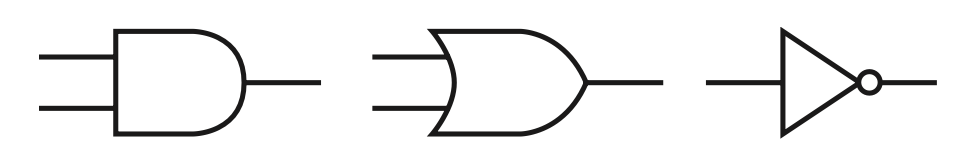
\includegraphics[width=0.5\linewidth]{img/gates.png}%
    }
    \caption{\textit{\texttt{AND} gate, \texttt{OR} gate, and inverter}}
\end{figure}

The gates can be combined to form different forms of logic. An example of this is $\overline{\overline{A} + B}$ which is equivalent to $A \cdot \overline{B}$ by De Morgan's law, seen in \autoref{fig:gates2}.

\begin{figure}[htbp]
    \centering
    \fcolorbox{codeFrame}{white}{
        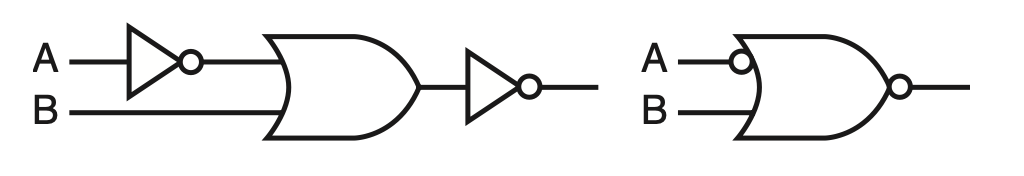
\includegraphics[width=0.5\linewidth]{img/gates2.png}%
    }
    \caption{\textit{Logic gate implementation of example formula}}
    \label{fig:gates2}
\end{figure}

\subsection*{Decoders \& Multiplexors}

A \textbf{decoder} is a logic block that has an n-bit input and $2^n$ outputs, where there is one unique true bit as output from a unique set of bytes of input.

\begin{figure}[htbp]
    \centering
    \fcolorbox{codeFrame}{white}{
        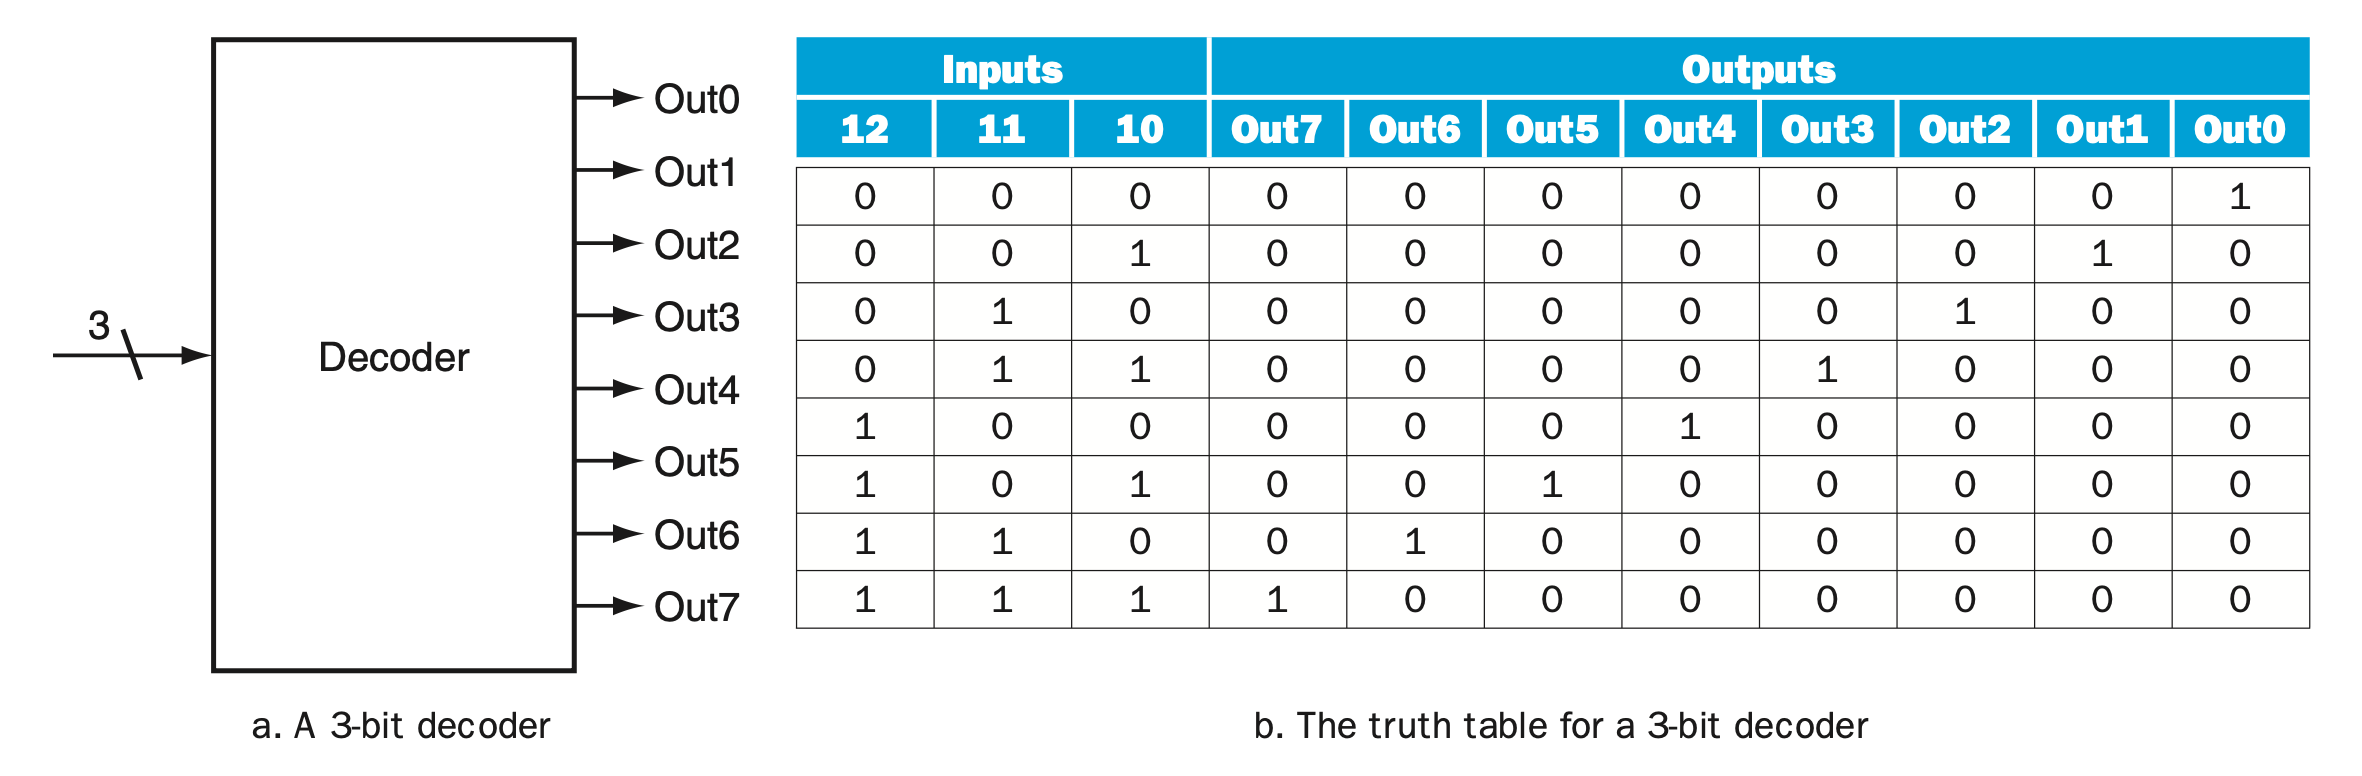
\includegraphics[width=0.7\linewidth]{img/decoder1.png}
    }
    \caption{\textit{3-bit input decoder that generates $2^3=8$ different outputs (Out0 – Out7)}}
\end{figure}

$$2^n \text{ outputs} \ \therefore \ \log_2{(\text{output})} = \text{input bits}$$

Encoders are the other way around.

\textbf{Multiplexors} have a selector input (or control value), that will determine which inputs will become outputs.

In the case of the two-input MUX, its representation is the following, $C=(A \cdot \overline{S}) +(B \cdot S)$, using n (data inputs) AND gates, and one OR gate.

\begin{figure}[htbp]
    \centering
    \fcolorbox{codeFrame}{white}{
        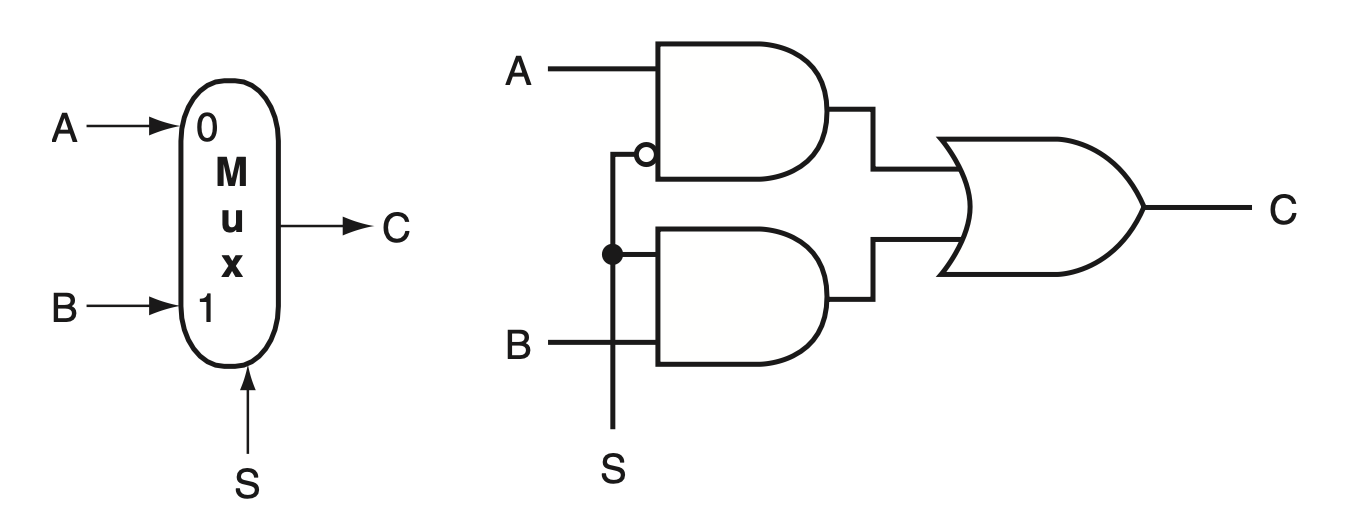
\includegraphics[width=0.5\linewidth]{img/mux1.png}
    }
    \caption{\textit{Two-input multiplexor that generates one output depending on the selector input S}}
\end{figure}

\vspace{-2.5em}
$$n \text{ (data inputs)} \therefore \log_2{n} = S \text{ selector bits required to represent all inputs}$$

Often times a decoder generates n bits for a MUX, to be used as a selector signal.

\subsection*{Buses}
\label{jmp:buses-general}

A collection of data lines that is treated as a single logical signal.

When showing a logic unit whose inputs and outputs are buses, the unit must be replicated a sufficient number of times to accommodate the width of the input.

You can use multiplexors to select between two buses, requiring n inputs to represent n-bit buses.

\begin{figure}[htbp]
    \centering
    \fcolorbox{codeFrame}{white}{
        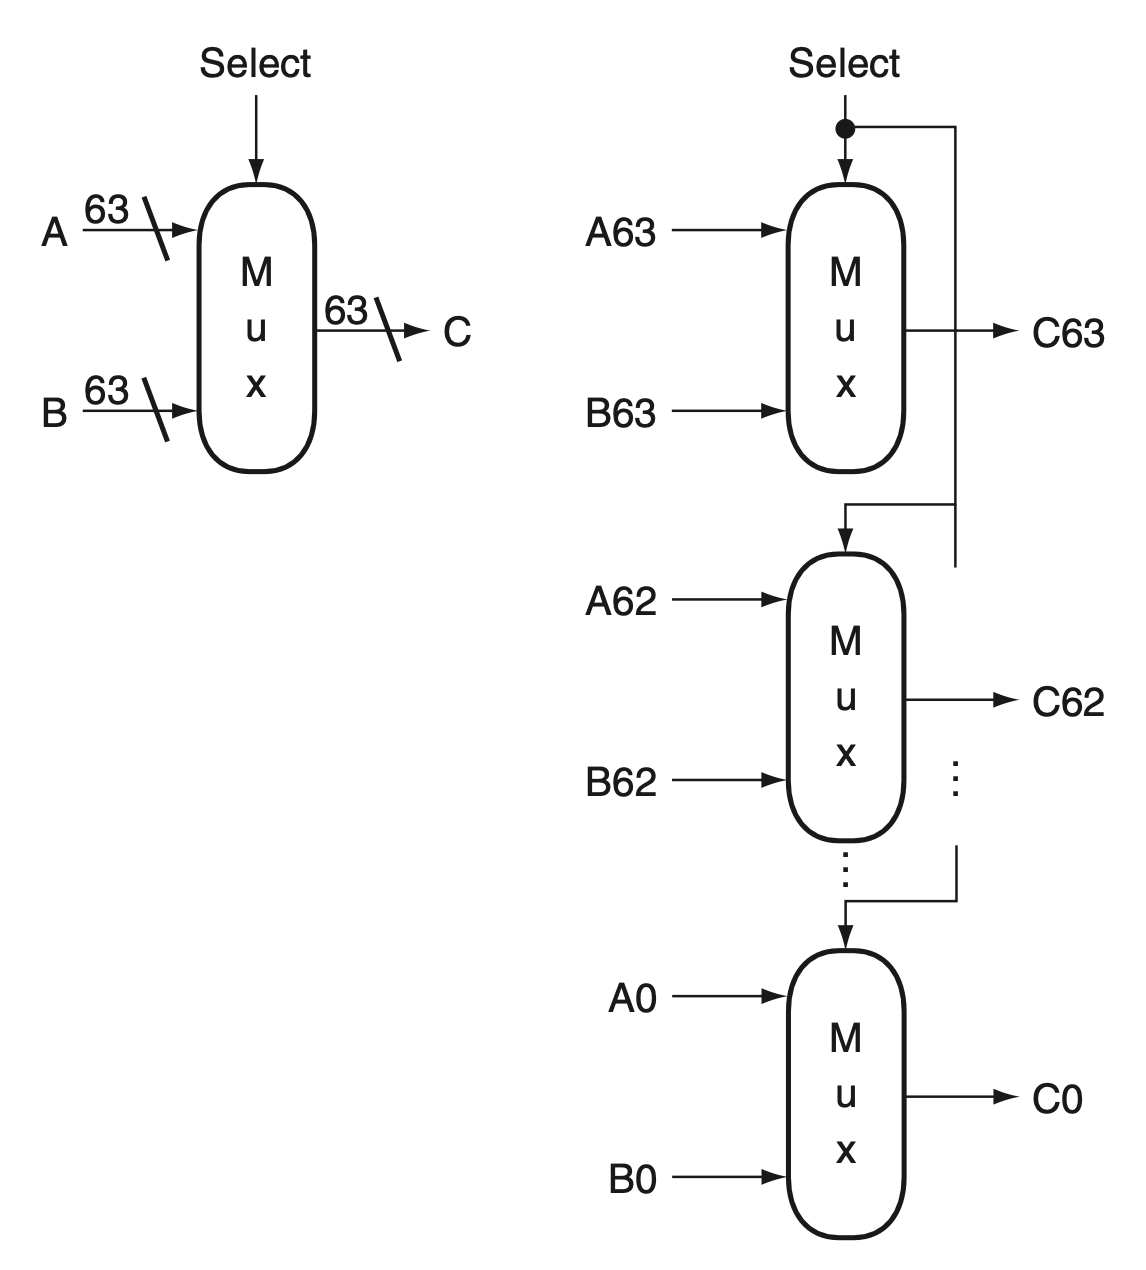
\includegraphics[width=0.28\linewidth]{img/bus1.png}
    }
    \caption{\textit{1-bit multiplexors replicated 64 times to represent two 64-bit buses}}
\end{figure}

\subsection*{ALUs}

\begin{tcolorbox}[
    enhanced,
    attach boxed title to top left={xshift=6mm,yshift=-1.5mm},
    colback=moonstoneblue!20,
    colframe=moonstoneblue,
    colbacktitle=moonstoneblue,
    title=Operation done by the ALU,
    fonttitle=\bfseries\color{white},
    boxed title style={size=small,colframe=moonstoneblue,sharp corners},
    sharp corners,
]
    {\color{moondark}\textbf{Logic operations}}: \texttt{AND} and \texttt{OR} gate operations, with \texttt{NOR} being available through an inversion of both input signals with \texttt{AInvert} and \texttt{BInvert} control signals. \\
    {\color{moondark}\textbf{Arithmetic operations}}: Addition and subtraction through the full adder, and \texttt{BInvert} control signal on one input for determining the type of operation.
\end{tcolorbox}

The LEGv8 word is 64 bits wide, as such a 64 bit wide ALU is required (64 1-bit ALUs).

In its simplest form, a \underline{1-bit logical unit} for \texttt{AND} and \texttt{OR} operations simply requires a multiplexor an a one bit control signal to select between the two operations ($2^1=2$).

\begin{figure}[htbp]
    \centering
    \fcolorbox{codeFrame}{white}{
        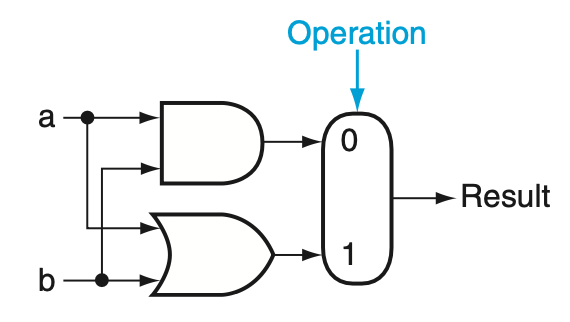
\includegraphics[width=0.28\linewidth]{img/alu1.png}
    }
    \caption{\textit{1-bit logical unit for \texttt{AND} and \texttt{OR} operations}}
\end{figure}

Implementing addition requires two input operands, one output, a \texttt{CarryIn} bit carried from the less-significant bits of the operation (i.e. another 1-bit logical unit), and a \texttt{CarryOut} bit to be carried forward to the next more significant bit.

\begin{figure}[htbp]
    \centering
    \fcolorbox{codeFrame}{white}{
        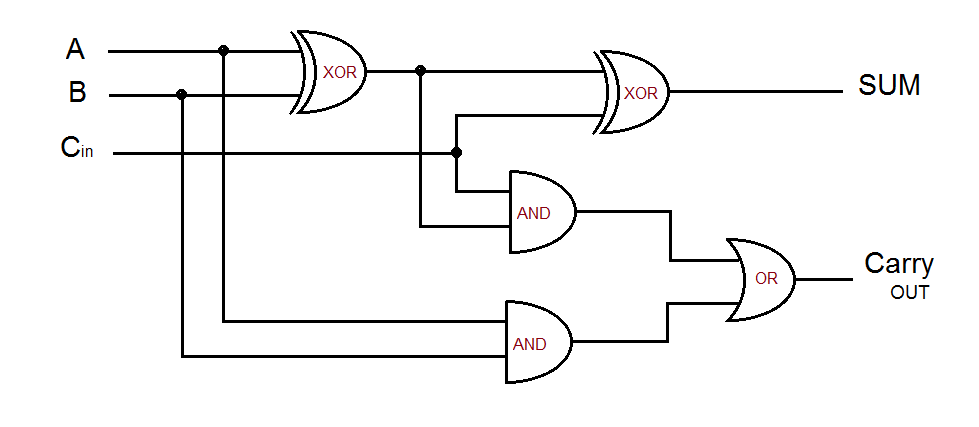
\includegraphics[width=0.8\linewidth]{img/adder1.png}
    }
    \caption{\textit{Full adder that performs mod 2 addition}}
\end{figure}

The combination of the adder and the logic gates, coupled with a multiplexor with a control signal to determine the operation makes a complete 1-bit ALU, which can be seen in \autoref{fig:1bitalu}.
\pagebreak

\begin{figure}[htbp]
    \centering
    \fcolorbox{codeFrame}{white}{
        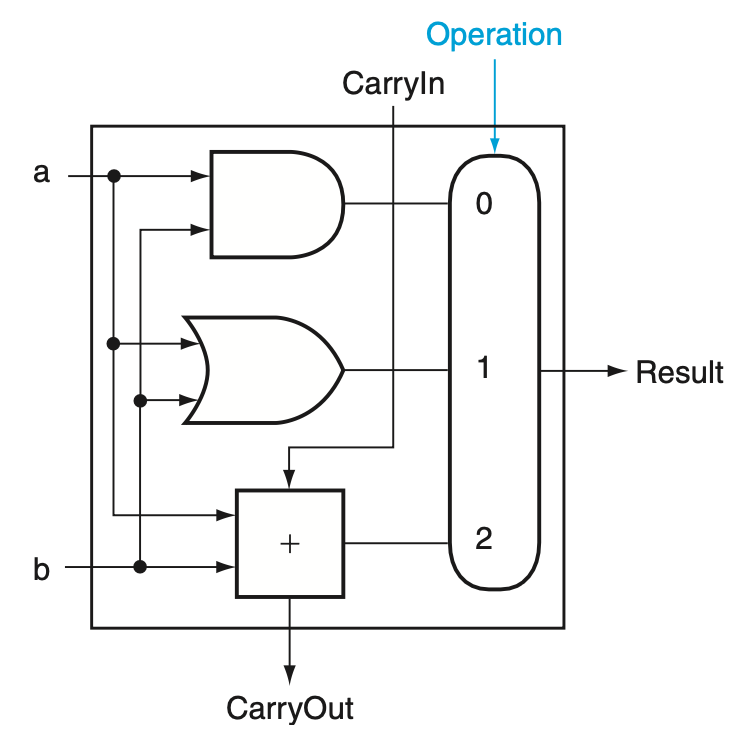
\includegraphics[width=0.2\linewidth]{img/alu2.png}
    }
    \caption{\textit{1-bit alu with logical operations and addition}}
    \label{fig:1bitalu}
\end{figure}

For expanding to a 64-bit ALU, the adders have to set up a ripple carry from the least to the most significant bit.

\begin{figure}[htbp]
    \centering
    \fcolorbox{codeFrame}{white}{
        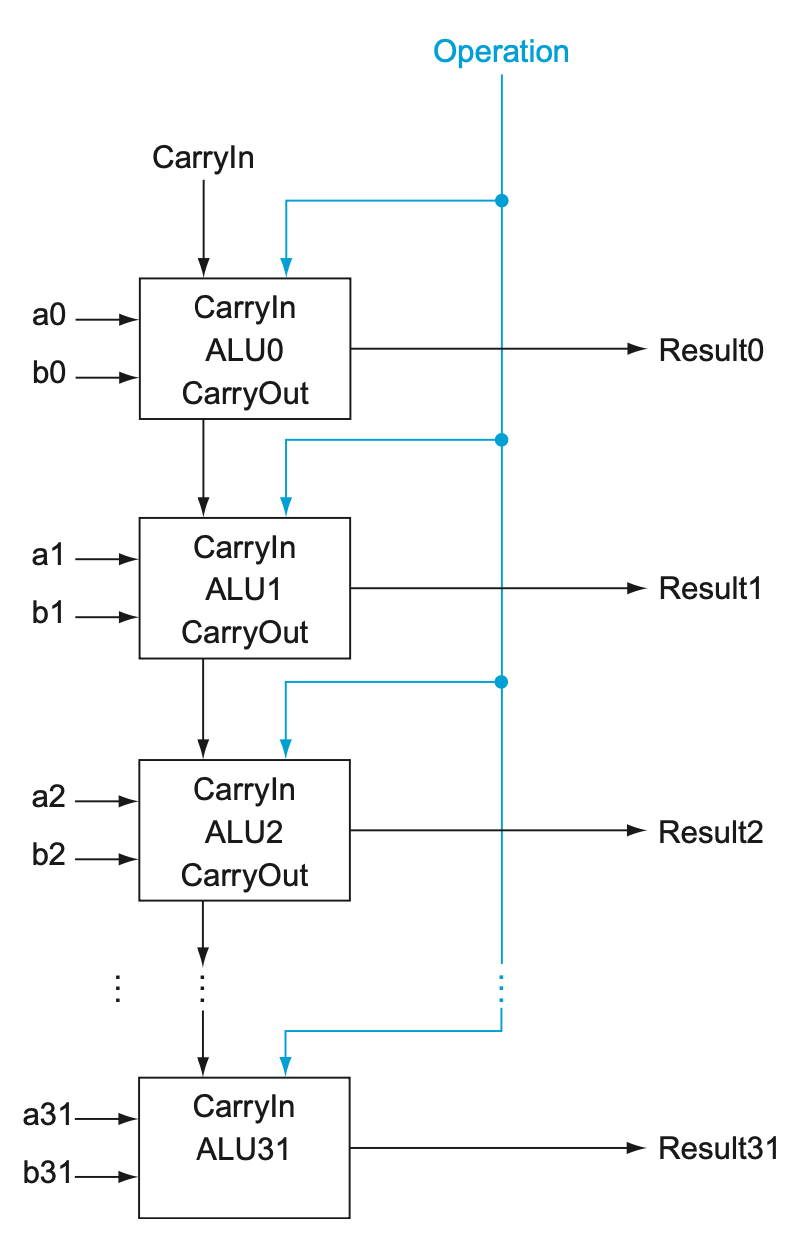
\includegraphics[width=0.2\linewidth]{img/ripplecarry.png}
    }
    \caption{\textit{Ripple carry implemented for a 64-bit ALU}}
\end{figure}

By inverting the second input (\texttt{BInvert} = 1, seen in \autoref{fig:subalu}) and setting \texttt{CarryIn} to 1 in the least significant bit of the ALU, we get two’s complement subtraction of \texttt{b} from \texttt{a}.

To implement a \texttt{NOR} function, existing components can be combined, $(\overline{a+b})=\overline{a} \cdot \overline{b}$ (DeMorgan's theorem), which means we need an \texttt{AND} and two inverters for both \texttt{a} and \texttt{b}, seen in \autoref{fig:subalu}

\begin{figure}[htbp]
    \centering
    \fcolorbox{codeFrame}{white}{
        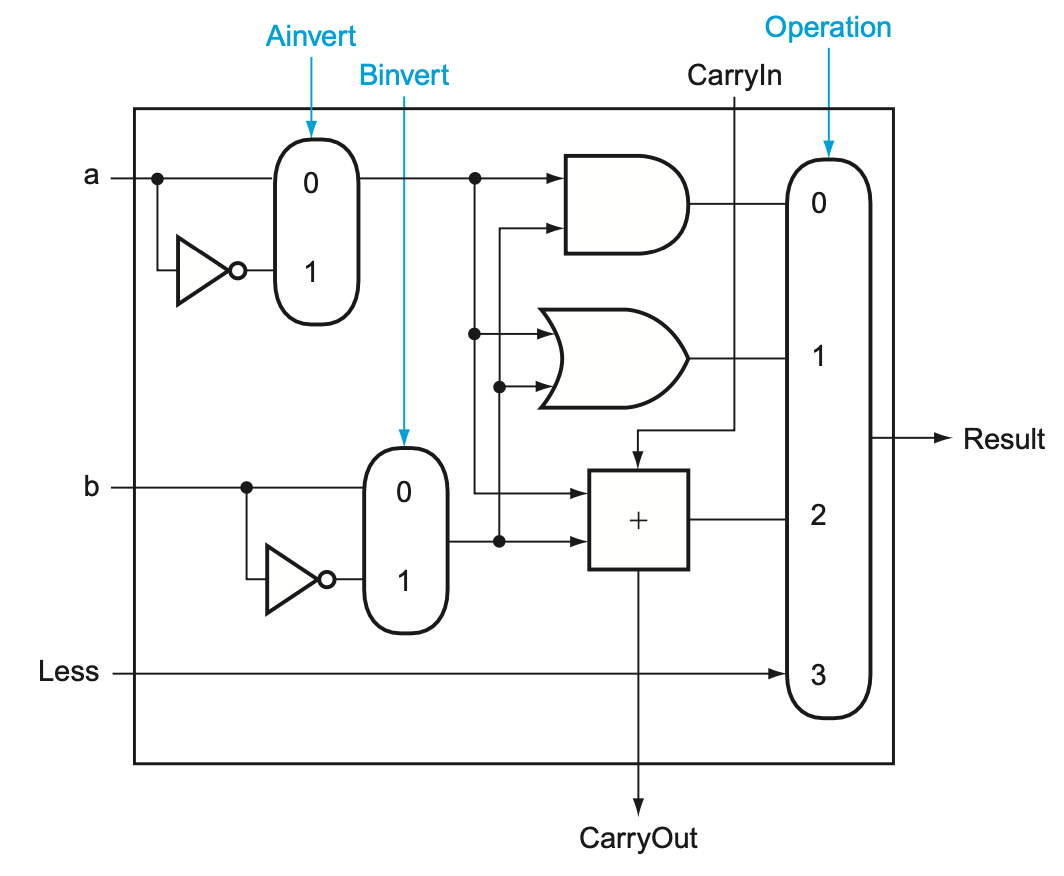
\includegraphics[width=0.32\linewidth]{img/alu3.png}
    }
    \caption{\textit{1-bit ALU that performs subtraction, and \texttt{NOR} operations}}
    \label{fig:subalu}
\end{figure}

On a 64-bit ALU we can use a zero flag \label{jmp:zero-flag} to help with conditional branch instructions in LEGv8 (e.g. \texttt{CBZ}), as they receive to inputs and require to test if the subtraction has a zero.

The following represents this with an inversion of an \texttt{OR} tree on all results from the subtraction considering a 64-bit subtraction, fully represented in \autoref{fig:64aluzero}.
\vspace{-1em}
$$Zero = \overline{(R_0 + R_1 + R_2 + ... + R_{63})}$$
\vspace{-3em}

\begin{figure}[htbp]
    \centering
    \fcolorbox{codeFrame}{white}{
       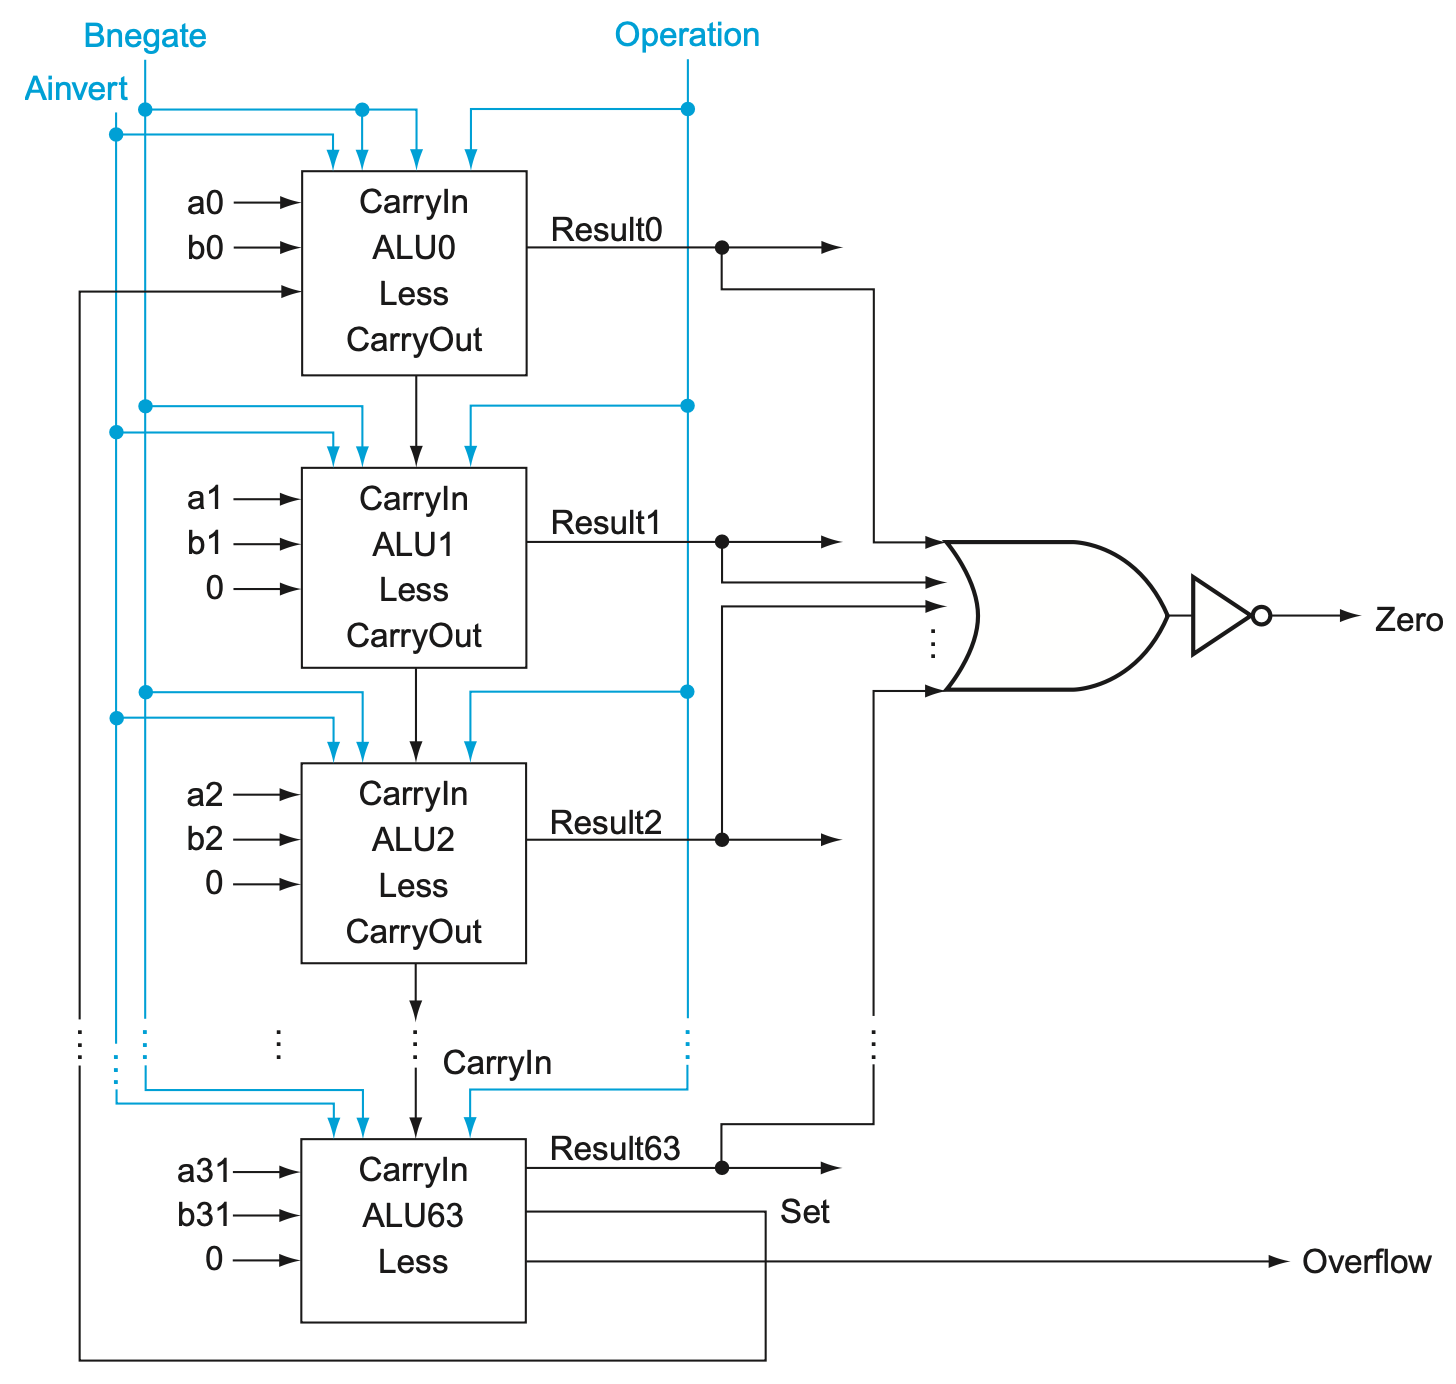
\includegraphics[width=0.4\linewidth]{img/alu4.png}
    }
    \caption{\textit{64-bit ALU \texttt{OR} tree and an inverter for determining the Zero flag}}
    \label{fig:64aluzero}
\end{figure}

For a generalized symbol of the ALU, \autoref{fig:generalalu}, where \texttt{ALU operation} is the control signal of the MUX that determines the type of operation.

\begin{figure}[htbp]
    \centering
    \fcolorbox{codeFrame}{white}{
       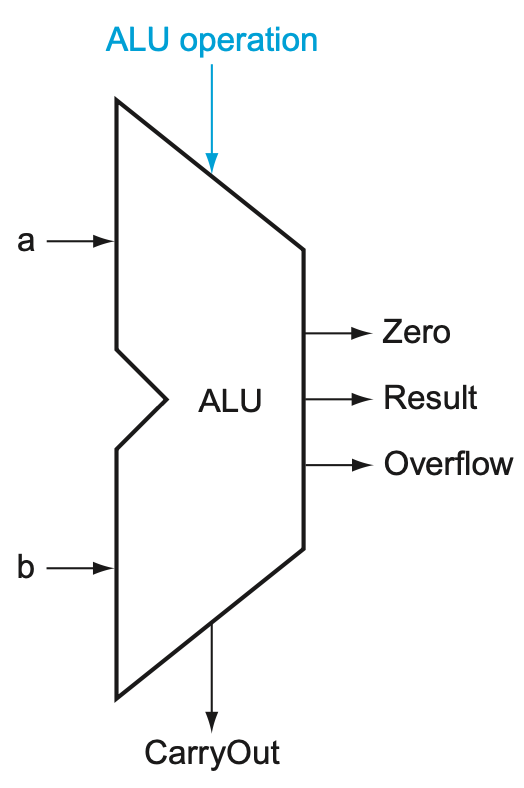
\includegraphics[width=0.2\linewidth]{img/alu5.png}
    }
    \caption{\textit{General symbol for an ALU or an adder}}
    \label{fig:generalalu}
\end{figure}

\pagebreak

\subsection*{Clocks}

\begin{tcolorbox}[
    enhanced,
    attach boxed title to top left={xshift=6mm,yshift=-1.5mm},
    colback=moonstoneblue!20,
    colframe=moonstoneblue,
    colbacktitle=moonstoneblue,
    title=Clocking methodology semantics,
    fonttitle=\bfseries\color{white},
    boxed title style={size=small,colframe=moonstoneblue,sharp corners},
    sharp corners,
]
    {\color{moondark}\textbf{Edge triggered clocking}}: State changes occur on a clock edge. \\
    {\color{moondark}\textbf{Synchronous system}}: Type of memory system where data is read only when a clock signal indicates stability (i.e. non-changing value).
\end{tcolorbox}

A \hyperref[box:logic-types]{combinational logic block}, recieves an input and then generates an output for a state element which is updated on a clock edge.

An edge-triggered methodology allows a state element to be read and written in the same clock cycle without creating a race condition.

For this to work, the clock cycle must be long enough for the state element to have received a stable input before the next active clock edge.

\begin{figure}[htbp]
    \centering
    \fcolorbox{codeFrame}{white}{
       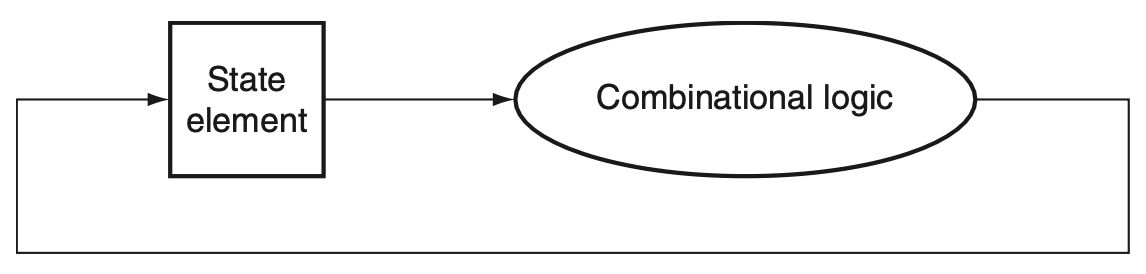
\includegraphics[width=0.5\linewidth]{img/clock1.png}
    }
    \caption{\textit{Edge-triggered state element to be read and written to in one active clock edge}}
\end{figure}

One such state element is the register file.

\subsection*{Flip-flops \& Latches}

\begin{tcolorbox}[
    enhanced,
    attach boxed title to top left={xshift=6mm,yshift=-1.5mm},
    colback=moonstoneblue!20,
    colframe=moonstoneblue,
    colbacktitle=moonstoneblue,
    title=Types of clocked memory elements,
    fonttitle=\bfseries\color{white},
    boxed title style={size=small,colframe=moonstoneblue,sharp corners},
    sharp corners,
]
    {\color{moondark}\textbf{Flip-flops}}: Edge-triggered element that changes the stored state only at a clock edge. \\
    {\color{moondark}\textbf{Latches}}: Level-sensitive element that changes the stored state at any time the clock is asserted.
\end{tcolorbox}

Flip-flops are build upon latches and are going to be used in edge-triggered systems.

A \textbf{D flip-flop} or \textbf{D latch} is used for storing the value of one data input signal, in the internal memory, at the clock edge.

To implement a \textbf{D latch}, it requires two inputs, the data to be stored \texttt{D}, and the clock signal \texttt{C}, producing two outputs, the value of the internal state \texttt{Q}, and its complement \(\overline{\mathtt{Q}}\).

The \hyperref[]{implementation} has cross-coupled \texttt{NOR} gates that store the state value unless \texttt{C} is asserted, in which case \texttt{D} replaces the value of \texttt{Q} and is stored.

\pagebreak

\begin{figure}[htbp]
    \centering
    \fcolorbox{codeFrame}{white}{
       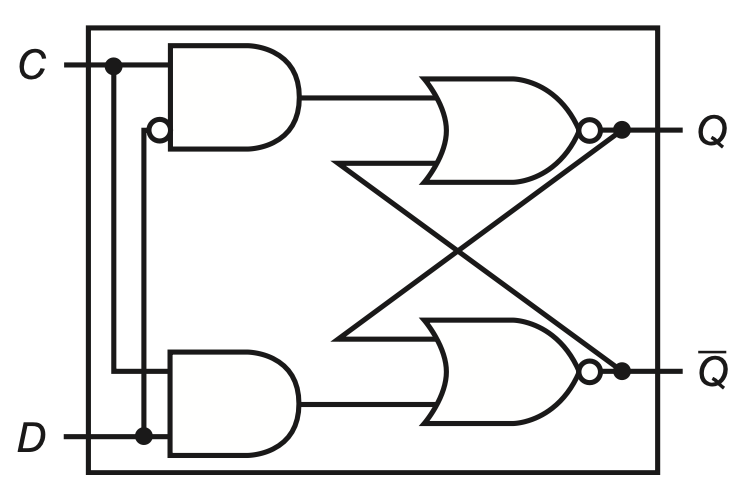
\includegraphics[width=0.3\linewidth]{img/dlatch.png}
    }
    \caption{\textit{D latch, composed of crossed \texttt{NOR} gates and a \texttt{SR} latch}}
    \vspace{1em}
    \centering
    \fcolorbox{codeFrame}{white}{
       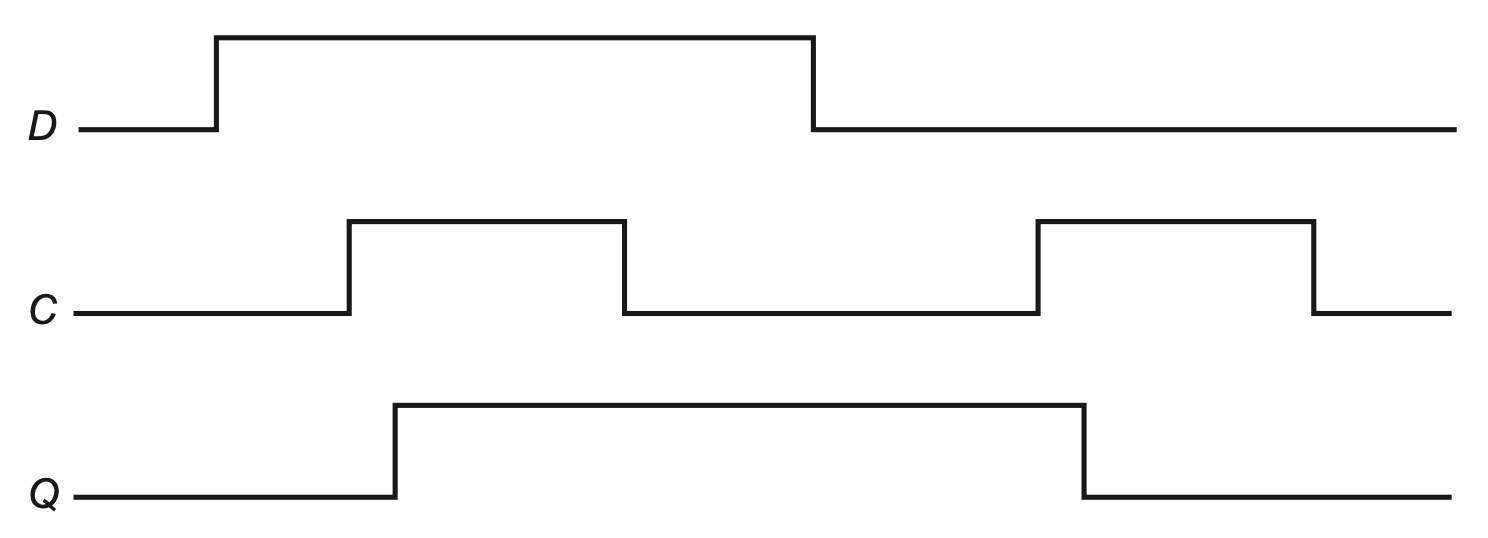
\includegraphics[width=0.35\linewidth]{img/dlatch1.png}
    }
    \caption{\textit{Progression of a D latch, assuming output is initially deasserted}}
\end{figure}

To implement a \textbf{D flip-flop}, with a \underline{falling-edge trigger}, we can use two D latches, master and slave. Master sets input \texttt{D} when \texttt{C} is asserted. When \texttt{C} falls, master is closed, but slave is open and gets its input from master's \texttt{Q}.

In this sense, the rising-edge represents when the master takes in the \texttt{D} value, and the falling-edge represents when the slave takes in the master's \texttt{D} producing the final \texttt{Q}.

\begin{figure}[htbp]
    \centering
    \fcolorbox{codeFrame}{white}{
       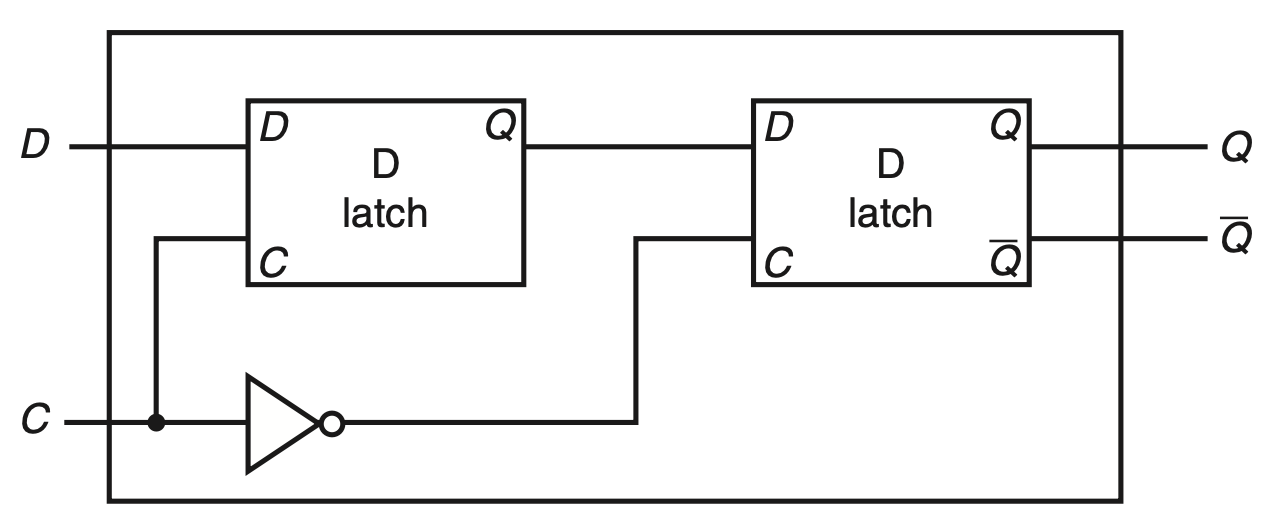
\includegraphics[width=0.5\linewidth]{img/dflip.png}
    }
    \caption{\textit{D flip-flop with a falling-edge trigger made from two D latches, master and slave}}
    \vspace{1.5em}
    \centering
    \fcolorbox{codeFrame}{white}{
       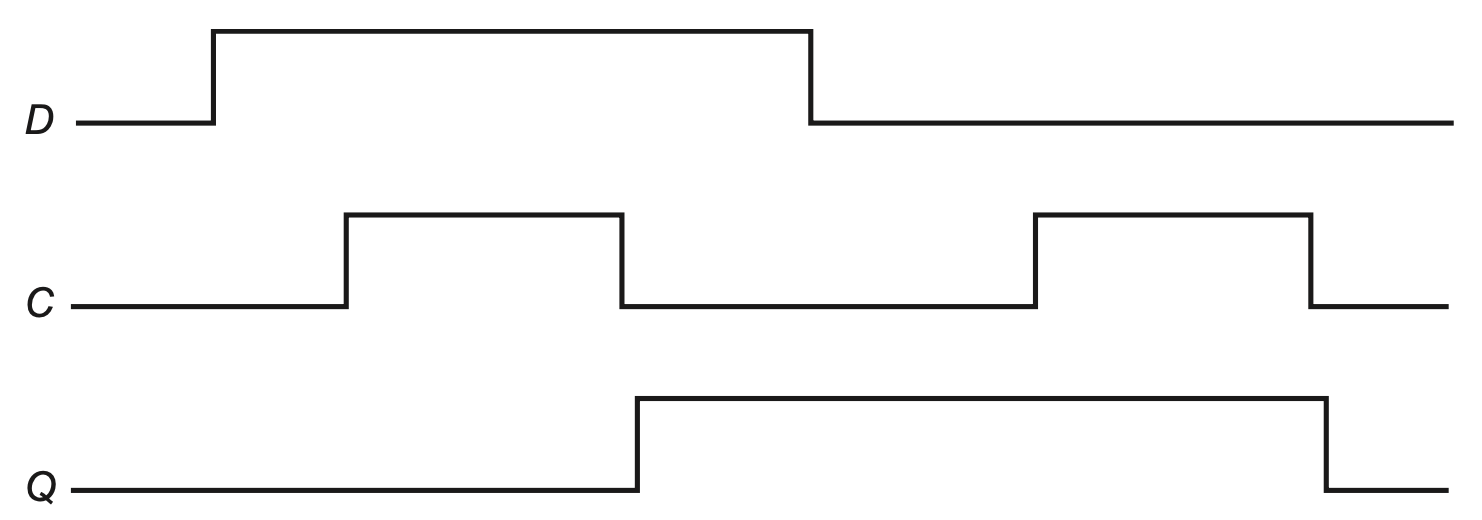
\includegraphics[width=0.5\linewidth]{img/dflip1.png}
    }
    \caption{\textit{Progression of a D flip-flop with a falling-edge trigger, where output is initially deasserted}}
\end{figure}

The minimum time \texttt{D} must retain a valid input is the setup time plus the hold time (after edge).

\subsection*{Register files}

A \textbf{register file} consists of a bunch of \textbf{registers} that can be read and written to, and a \texttt{WriteReg} control signal (clock).

For writing it requires the control signal, the number of the register to write to (\texttt{Write register}), and the data to write (\texttt{Write data}).

For reading it requires the numbers of the registers to read from (\texttt{Read register number 1 \& 2}), and it outputs the read contents from two registers (\texttt{Read data 1 \& 2}).

\begin{figure}[htbp]
    \centering
    \fcolorbox{codeFrame}{white}{
       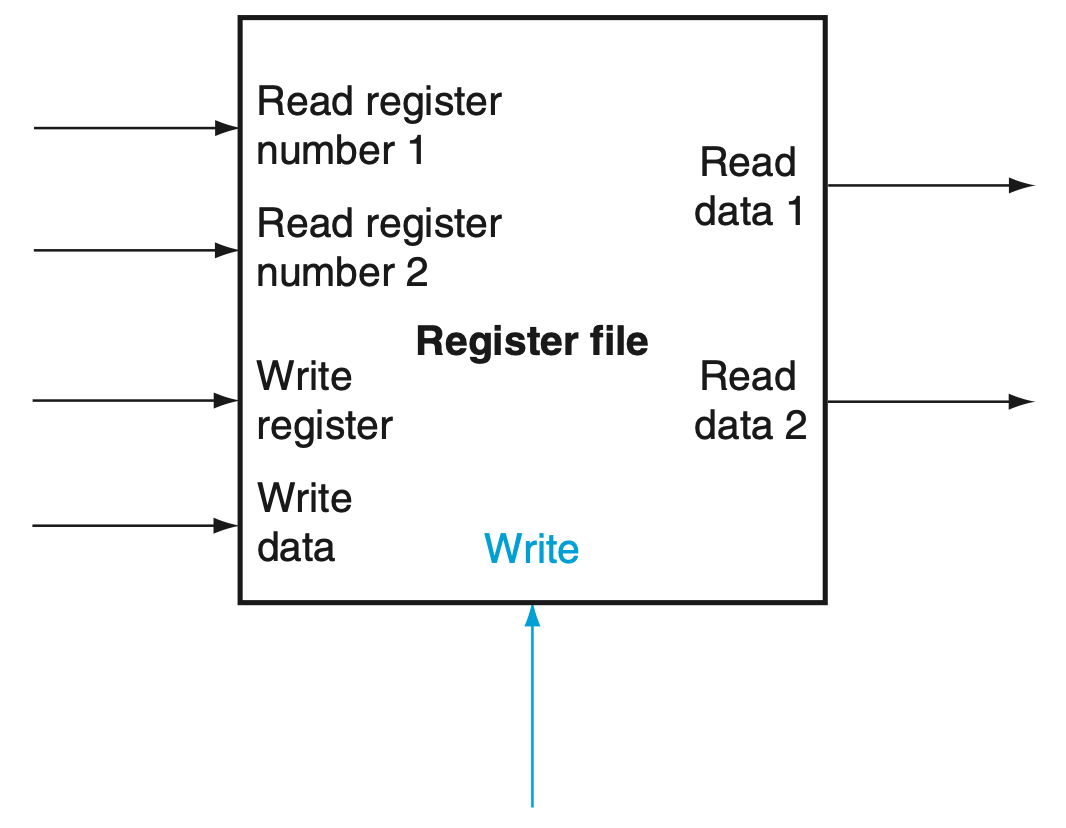
\includegraphics[width=0.35\linewidth]{img/regfile1.png}
    }
    \caption{\textit{Register file with two read ports and one write port}}
\end{figure}

The implementation for the \underline{write port} consists of a decoder that will select one of the \texttt{n - 1} registers that will be \texttt{AND}ed with the \texttt{WriteReg} signal to act as the \texttt{C} input for the registers (D flip-flops). The \texttt{D} input for every register is the \texttt{Write data} input from the reg. file.

\begin{figure}[htbp]
    \centering
    \fcolorbox{codeFrame}{white}{
       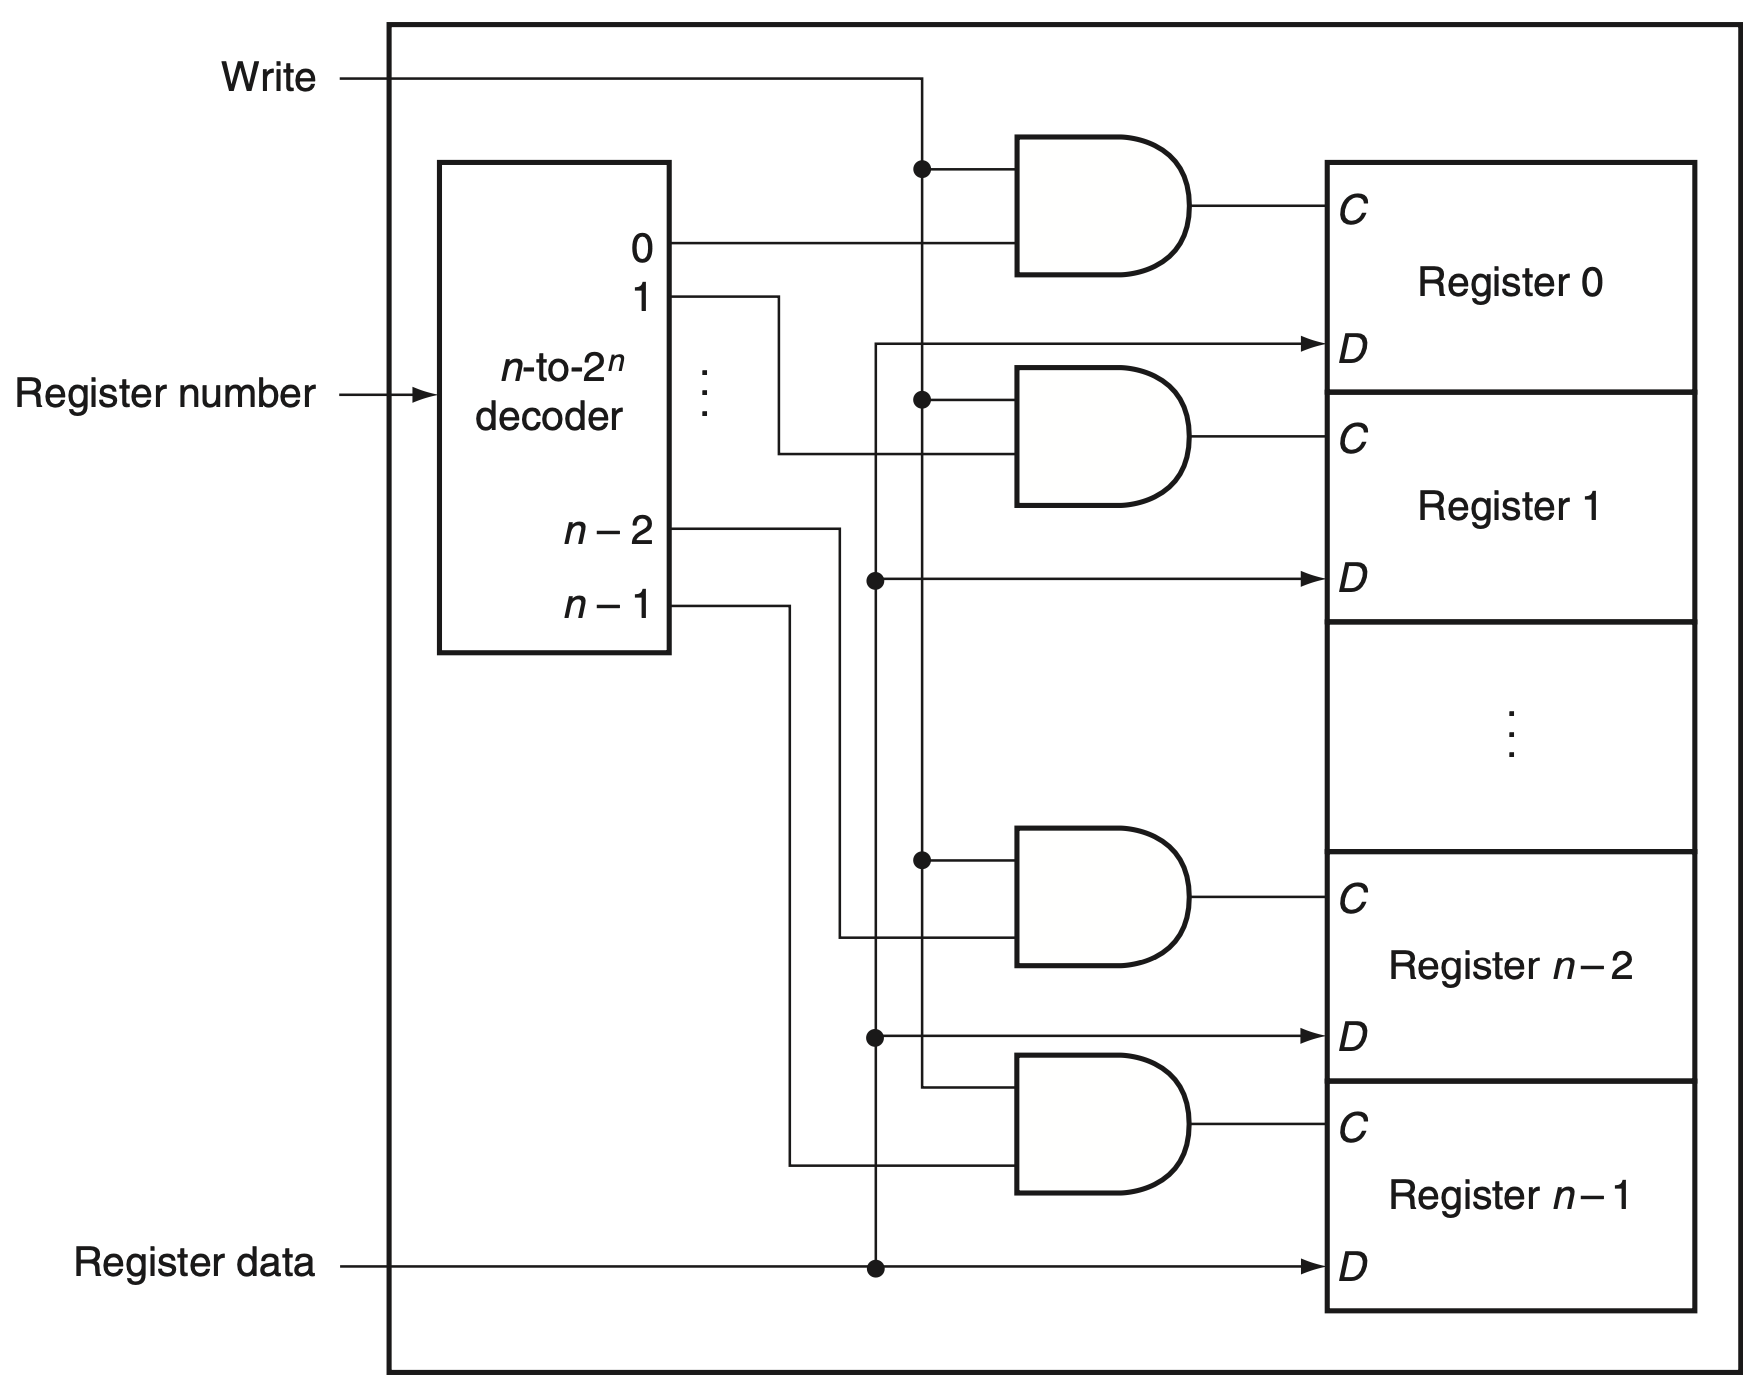
\includegraphics[width=0.55\linewidth]{img/regwrite1.png}
    }
    \caption{\textit{Write implementation in the register file}}
\end{figure}

The implementation for the two \underline{read ports} consists of using the stored state of the registers (\texttt{Q} output), as inputs for two different MUXes that use the \texttt{Read register number 1 \& 2} reg. file inputs as control signals to output the information of the two registers specified.

\begin{figure}[htbp]
    \centering
    \fcolorbox{codeFrame}{white}{
       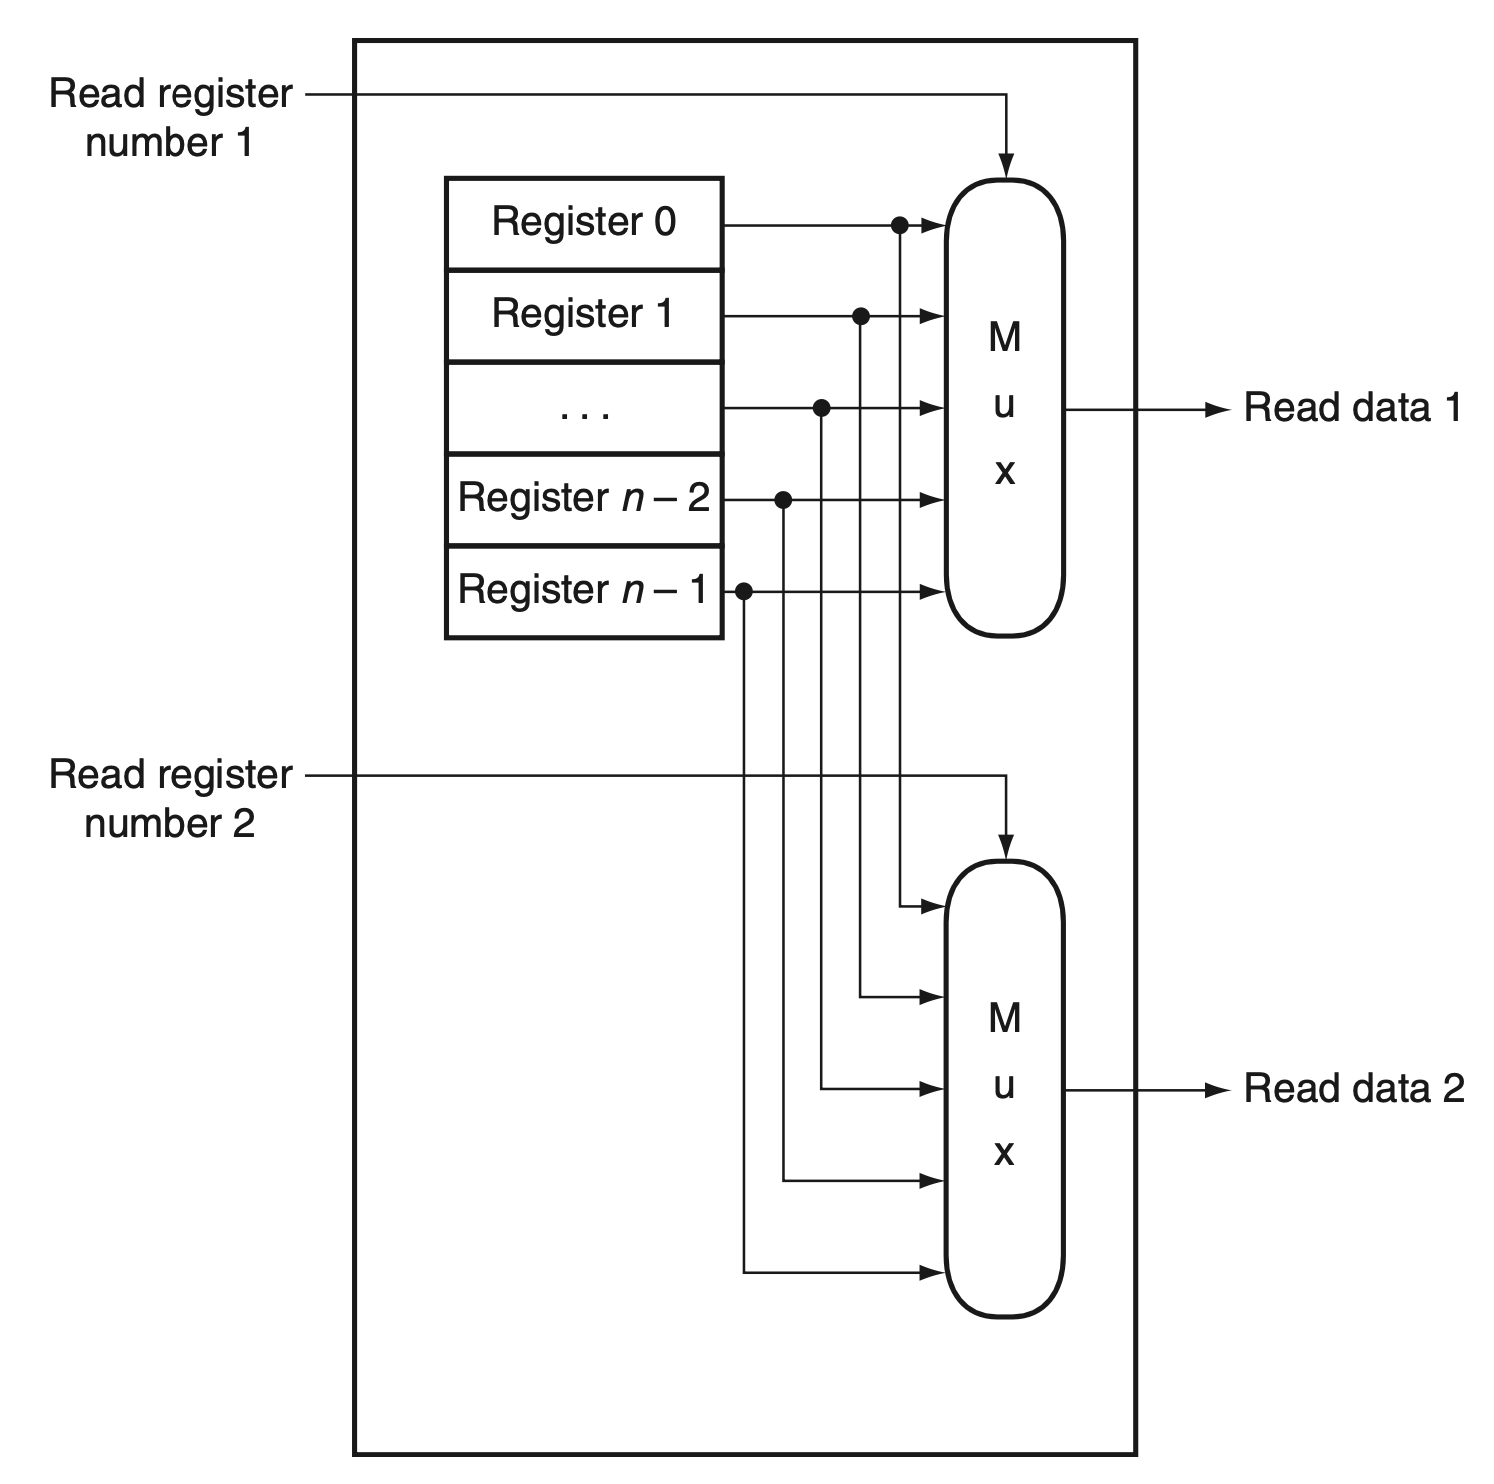
\includegraphics[width=0.55\linewidth]{img/regread1.png}
    }
    \caption{\textit{Read implementation in the register file}}
\end{figure}

\pagebreak

\section*{Chapter 2}
\addcontentsline{toc}{section}{Chapter 2}

The size of a register in LEGv8 is 64 bits, which are denominated as doublewords (8 bytes).

A word, the natural unit of access in a computer, is 32 bits (4 bytes).

\subsection*{LEGv8 Assembly}

\begin{tcolorbox}[
    enhanced,
    attach boxed title to top left={xshift=6mm,yshift=-1.5mm},
    colback=moonstoneblue!20,
    colframe=moonstoneblue,
    colbacktitle=moonstoneblue,
    title=Relevant LEGv8 instructions,
    fonttitle=\bfseries\color{white},
    boxed title style={size=small,colframe=moonstoneblue,sharp corners},
    sharp corners,
]
    \begin{tabular}{@{} l @{\quad} l @{}}
    {\color{moondark}\textbf{Addition}}:           & \texttt{ADD X1, X2, X3}     \\
    {\color{moondark}\textbf{Subtraction}}:        & \texttt{SUB X1, X2, X3}     \\
    {\color{moondark}\textbf{Add immediate}}:      & \texttt{ADDI X1, X2, \#20}  \\
    {\color{moondark}\textbf{Subtract immediate}}: & \texttt{SUBI X1, X2, \#20}  \\
    {\color{moondark}\textbf{Load register}}:      & \texttt{LDUR X1, [X2, \#20] \ \ // Load mem. at addrs. X2 + 20} \\
    {\color{moondark}\textbf{Store register}}:     & \texttt{STUR X1, [X2, \#20] \ \ // Store at addrs. X2 + 20} \\
    {\color{moondark}\textbf{Logical AND}}:        & \texttt{AND X1, X2, X3}  \\
    {\color{moondark}\textbf{Logical Inclusive OR}}: & \texttt{ORR X1, X2, X3}  \\
    {\color{moondark}\textbf{Logical Exclusive OR}}: & \texttt{EOR X1, X2, X3}  \\
    {\color{moondark}\textbf{Bitwise Left}}:       & \texttt{LSL X1, X2, \#20}  \\
    {\color{moondark}\textbf{Bitwise Right}}:      & \texttt{LSR X1, X2, \#20}  \\
    {\color{moondark}\textbf{Conditional branch is 0}}: & \texttt{CBZ X1, L0 \ \ // Inmediate in operand is in word bytes} \\
    {\color{moondark}\textbf{Conditional branch not 0}}: & \texttt{CBNZ X1, L0 \ \ // Inmediate in operand is in word bytes} \\
    {\color{moondark}\textbf{Branch}}:             & \texttt{B L0 \ \ // Inmediate in operand is in word bytes}
    \end{tabular}
\end{tcolorbox}

The above list excludes instructions that set flags, e.g. \texttt{ADDS, SUBS, SUBIS, ADDIS}, and zero independent conditional branching, e.g. \texttt{B.cond}.

\subsection*{LEGv8 architecture design}

There are 32 64-bit registers, limited as larger number of registers implies increasing clock cycle time as electronic signals take longer as they must travel further. It also makes instruction formats more constrained.

Many architectures have alignment restriction that establish that words must start at addresses that are multiples of 4 and doublewords at multiples of 8.

\pagebreak

\subsection*{Signed and unsigned numbers}

\begin{tcolorbox}[
    enhanced,
    attach boxed title to top left={xshift=6mm,yshift=-1.5mm},
    colback=moonstoneblue!20,
    colframe=moonstoneblue,
    colbacktitle=moonstoneblue,
    title=Denomination of bits in a bit string,
    fonttitle=\bfseries\color{white},
    boxed title style={size=small,colframe=moonstoneblue,sharp corners},
    sharp corners,
    label=box:logic-types,
]
    {\color{moondark}\textbf{Least significant bit}}: The rightmost bit in a bit string. In a doubleword this is bit 63. \\
    {\color{moondark}\textbf{Most significant bit}}: The leftmost bit in a bit string. In a doubleword this is bit 0.
\end{tcolorbox}

A \textbf{sign and magnitude} representation of a signed number has one bit set aside to represent the sign of the integer. Issues come with having a \texttt{-0} and \texttt{+0}, and more steps needed to determine the sign by the adder.

For making the hardware simple, \textbf{two's complement} representation is used, which used leading \texttt{0}s to denote positives, and leading \texttt{1}s to denote negatives. This means that the most significant bit can be used as a sign bit, making conversions the following way.

\vspace{-1em}
$$(x_{63} \cdot -2^{63})+(x_{62} \cdot 2^{62})+(x_{61} \cdot 2^{61})+...+(x_{1} \cdot 2^{1})+(x_{0} \cdot 2^{0})$$

As an example,
\vspace{-1em}
$$11111111 \ 11111111 \ 11111111 \ 11111111 \ 11111111 \ 11111111 \ 11111111 \ 11111100_{\text{two}}=-4_{\text{ten}}$$

\underline{Overflow} occurs when the sign bit gets overridden, i.e. \texttt{0} when negative, \texttt{1} when positive.

Using two's complement, \underline{sign extension}, used for conditional branching, just requires to copy the sign bit \texttt{m - n} bits over, where \texttt{m} is the new size of the bit string.

\begin{tcolorbox}[
    enhanced,
    attach boxed title to top left={xshift=6mm,yshift=-1.5mm},
    colback=moonstoneblue!20,
    colframe=moonstoneblue,
    colbacktitle=moonstoneblue,
    title=Power of 2 prefix definitions,
    fonttitle=\bfseries\color{white},
    boxed title style={size=small,colframe=moonstoneblue,sharp corners},
    sharp corners,
    label=box:logic-types,
]
    {\color{moondark}\textbf{Kibibyte (Kib)}}: $2^{10}$ bytes. \\
    {\color{moondark}\textbf{Mebibyte (Mib)}}: $2^{20}$ bytes. \\
    {\color{moondark}\textbf{Gibibyte (Gib)}}: $2^{30}$ bytes. \\
    {\color{moondark}\textbf{Tebibyte (Tib)}}: $2^{40}$ bytes. \\
    {\color{moondark}\textbf{Pebibyte (Pib)}}: $2^{50}$ bytes.
\end{tcolorbox}

\pagebreak

\subsection*{Instruction format fields}

\begin{table}[htbp]
  \centering

  \begin{minipage}[t]{0.45\textwidth}
    \centering
    \begin{tabular}{|l|l|l|l|l|}
      \hline
      \texttt{Opcode} & \texttt{Rm} & \texttt{shamt} & \texttt{Rn} & \texttt{Rd} \\
      11 bits & 5 bits & 6 bits  & 5 bits  & 5 bits \\
      \hline
    \end{tabular}
    \captionof{table}{\textit{R‐type format, \texttt{ADD, SUB, LSL, LSR}}}
  \end{minipage}\hfill
  \begin{minipage}[t]{0.45\textwidth}
    \centering
    \begin{tabular}{|l|l|l|l|l|}
      \hline
      \texttt{Opcode} & \texttt{Address} & \texttt{Op2} & \texttt{Rn} & \texttt{Rt} \\
      11 bits & 9 bits & 2 bits  & 5 bits  & 5 bits \\
      \hline
    \end{tabular}
    \captionof{table}{\textit{D‐type format, \texttt{LDUR, STUR}}}
  \end{minipage}

  \vspace{1em}

  \begin{minipage}[t]{0.45\textwidth}
    \centering
    \begin{tabular}{|l|l|l|l|}
      \hline
      \texttt{Opcode} & \texttt{Immediate} & \texttt{Rn} & \texttt{Rd} \\
      10 bits & 12 bits & 5 bits  & 5 bits \\
      \hline
    \end{tabular}
    \captionof{table}{\textit{I‐type format, \texttt{ADDI, SUBI}}}
  \end{minipage}\hfill
  \begin{minipage}[t]{0.45\textwidth}
    \centering
    \begin{tabular}{|l|l|l|}
      \hline
      \texttt{Opcode} & \texttt{Address} & \texttt{Rd} \\
      8 bits & 19 bits & 5 bits \\
      \hline
    \end{tabular}
      \captionof{table}{\textit{Conditional branch format, \texttt{CB(N)Z}}}
  \end{minipage}

  \vspace{1em}

  \begin{minipage}[t]{0.5\textwidth}
    \centering
    \begin{tabular}{|l|l|}
      \hline
      \texttt{Opcode} & \texttt{Address} \\
      6 bits & 26 bits \\
      \hline
    \end{tabular}
    \captionof{table}{\textit{Unconditional branch format, \texttt{B}}}
  \end{minipage}

\end{table}

All instruction field formats are 32 bits, thus the name \textit{32-bit instructions}.

The \texttt{opcode} denotes the operation and format of an instruction.

The register operands, \texttt{Rn}, \texttt{Rm}, and \texttt{Rd} are 5 bits to represent the 32 registers ($\log_2{32}=5$).

The \texttt{address} field can represent a region of $\pm2^8$ bytes around the base register \texttt{Rn}.

The \texttt{shamt} field represents the shift amount used by bit-shift instructions.

\subsection*{Conditional Statement \& Loops}

\begin{lstlisting}[caption={Simple conditional statement implementation}]
    CBNZ X3, Else       // if (X3 == 0) {
    ADD  X0, X1, X2     //     X0 = X1 + X2;
    B    Exit           // }
Else:                   // else {
    SUB  X0, X1, X2     //     X0 = X1 - X2;
Exit:                   // }
\end{lstlisting}


\begin{lstlisting}[caption={Simple while loop implementation}]
    ADDI X0, XZR, #10   // X0 = 10;
Loop:
    CBZ  X0, Exit       // while (X0 != 0) {
    SUBI X0, X0, #1     //     X0 -= 1;
    ADD  X1, X2, X0     //     X1 = X2 + X0;
    B    Loop           // }
Exit:
\end{lstlisting}

For a more complete example, the following converts the C code into LEGv8 assembly instructions.

\begin{lstlisting}[caption={C code loop into LEGv8 ASM}]
// C
int i = 0;
int k = 10;
while (save[i] == k) {
    i += 1;
}

// X25: Address of save[]

// Textbook LEGv8 ASM
    ADDI X22, XZR, #0   // EOR X22, X22, X22
    ADDI X14, XZR, #10
Loop:
    LSL  X10, X22, #2
    ADD  X10, X10, X25
    LDUR X11, [X10, #0]
    SUB  X12, X10, X14
    CBNZ X12, Exit
    ADDI X22, X22, #1
    B    Loop
Exit:

// Alternate LEGv8 ASM
    ADD  X10, XZR, X25
    ADDI X11, XZR, #10
Loop:
    LDUR X12, [X10, #0]
    SUB  X12, X12, X11
    CBNZ X12, Exit
    ADDI X10, X10, #8
    B Loop
Exit:
\end{lstlisting}

You can "throw away" the result by writing into \texttt{XZR}, the zero register.

\subsection*{Set Flag Branching}

The conditional branch instruction, \texttt{B.cond}, allows for \texttt{.cond} to be used for signed comparisons, \texttt{EQ} (equals), \texttt{NE} (not equal), \texttt{LT} (less than), \texttt{LE} (less than or equal), \texttt{GT}, or \texttt{GE}.

Also it allows for unsigned comparisons, \texttt{LO}, \texttt{LS} (lower or same), \texttt{HI}, or \texttt{HS} (higher or same).

The flag for comparison is set by instructions like, \texttt{ADDS}, \texttt{ADDIS}, or \texttt{SUBS}, but they are limited in number as they create dependencies that obstruct pipelining execution.

A use case is bounds checking, that is, $0\le x < y$.
\pagebreak

\begin{lstlisting}[caption={Bounds checking shortcut in LEGv8 ASM}]
// Pseudo C
if (X20 >= X11 || X20 < 0) {
    goto Error;
}

// LEGv8 ASM
    SUBS XZR, X20, X11
    B.HS Error
    B    Exit
Error:
    // Error handling
Exit:
\end{lstlisting}

Signed negative numbers look massive when looked at from an unsigned comparison in two's complement, and it also allows for checking if it is below a number (\texttt{X11} in example).

\pagebreak

\section*{Chapter 3}
\addcontentsline{toc}{section}{Chapter 3}

\subsection*{Floating point representation}

Compromise must be found between the size of the \textit{fraction} and the \textit{exponent}.

\begin{tcolorbox}[
    enhanced,
    attach boxed title to top left={xshift=6mm,yshift=-1.5mm},
    colback=moonstoneblue!20,
    colframe=moonstoneblue,
    colbacktitle=moonstoneblue,
    title=Tradeoff of floating-point representation,
    fonttitle=\bfseries\color{white},
    boxed title style={size=small,colframe=moonstoneblue,sharp corners},
    sharp corners,
    label=box:logic-types,
]
    {\color{moondark}\textbf{Precision}}: Increased by an increase in the size for the \textit{mantissa} or \textit{fraction}. \\
    {\color{moondark}\textbf{Range}}: Increased by an increase in the size for the \textit{exponent}.
\end{tcolorbox}

A LEGv8 implementation of \textbf{floating-point} numbers has \texttt{s} as the sign bit, \texttt{exponent} an 8-bit with bias, and \texttt{fraction} a 23-bit number.

\begin{figure}[htbp]
    \centering
    \fcolorbox{codeFrame}{white}{
       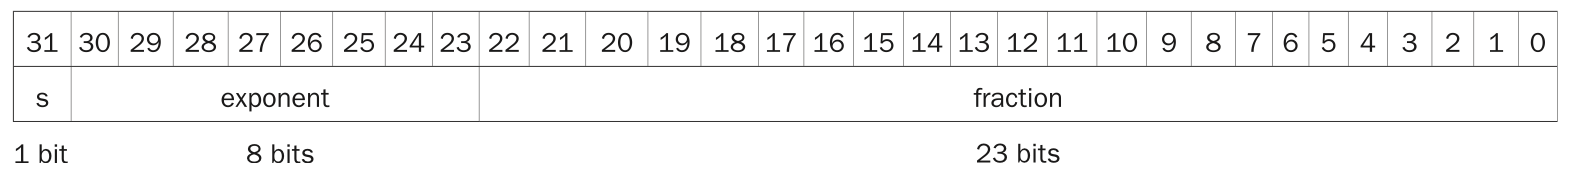
\includegraphics[width=0.7\linewidth]{img/legv8-float.png}
    }
    \caption{\textit{LEGv8 floating-point representation}}
\end{figure}
\vspace{-2em}
$$(-1)^S \times F \times 2^E$$

Range of representation is $2_{\text{ten}} \times 10^{38}$ considering $2^7 (\text{exponent 8-bit rep. divided by 2 for bias}) \approx 38$

Overflow entails the exponent being too large for the \texttt{exponent (E)} field to represent it. Underflow is the same situation but the \texttt{exponent} field representing a negative value.

To reduce the chances of underflow or overflow we use \textbf{double precision}, which is a floating-point value represented in a 64-bit doubleword.

\begin{figure}[htbp]
    \centering
    \fcolorbox{codeFrame}{white}{
       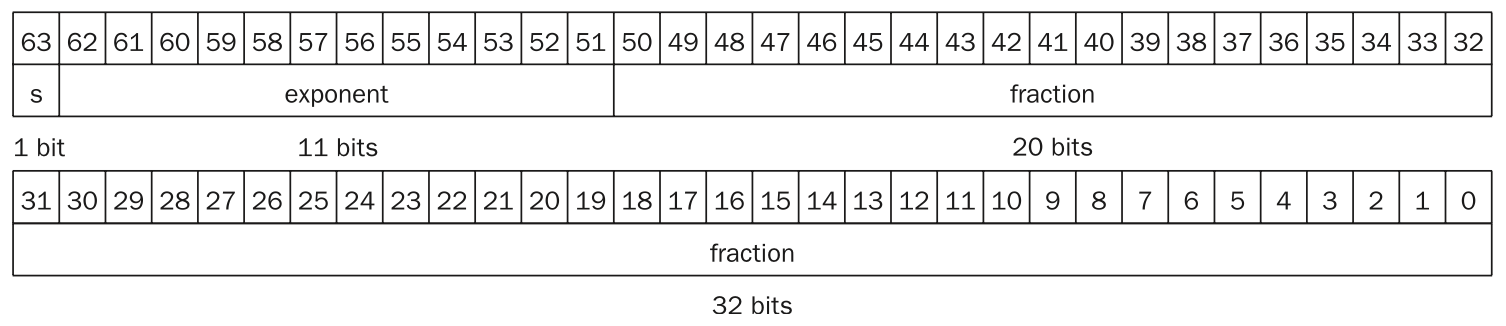
\includegraphics[width=0.85\linewidth]{img/doublep1.png}
    }
    \caption{\textit{LEGv8 double precision floating-point representation}}
\end{figure}

In the case of an overflow/underflow an interrupt (unscheduled disruption call) saves the address of the instruction (to resume after correction) and jumps to a predefined address that deals with the exception.

\subsection*{IEEE 754 Floating-Point Standard Specifications}

The floating-point can always have a leading \texttt{1.0}, as such IEEE assumes it as a hidden bit increasing the representation for the \texttt{fraction} by 1 (23 to 24 in single p., or 52 to 53 in double p.).

\vspace{-2em}
$$(-1)^S \times (1 + F) \times 2^{(\text{Exponent} - \text{Bias})}$$
\vspace{-2em}
$$(-1)^S \times (1 + (s1 \times 2^{-1}) + (s2 \times 2^{-2}) + ...) \times 2^E$$

IEEE 754 has \texttt{NaN} for invalid operations (e.g. $\frac{0}{0}$). Infinities can be represented through the largest exponent representations (+/$-$) instead of interrupting.

The sign bit is the most significant bit to easily process integer comparisons.

For representing the exponent without needing a sign bit, IEEE 754 uses a bias of 127 for single, and 1023 for double, that subtracts from the total possible representation to denote negative and positive exponents.

So for single precision, an exponent of $-1$ is $-1 + 127_{\text{ten}} = 126_{\text{ten}}$, and $+1$ is $1 + 127_{\text{ten}} = 128_{\text{ten}}$

\subsection*{Floating-Point Addition}

\begin{figure}[htbp]
    \centering
    \fcolorbox{codeFrame}{white}{
       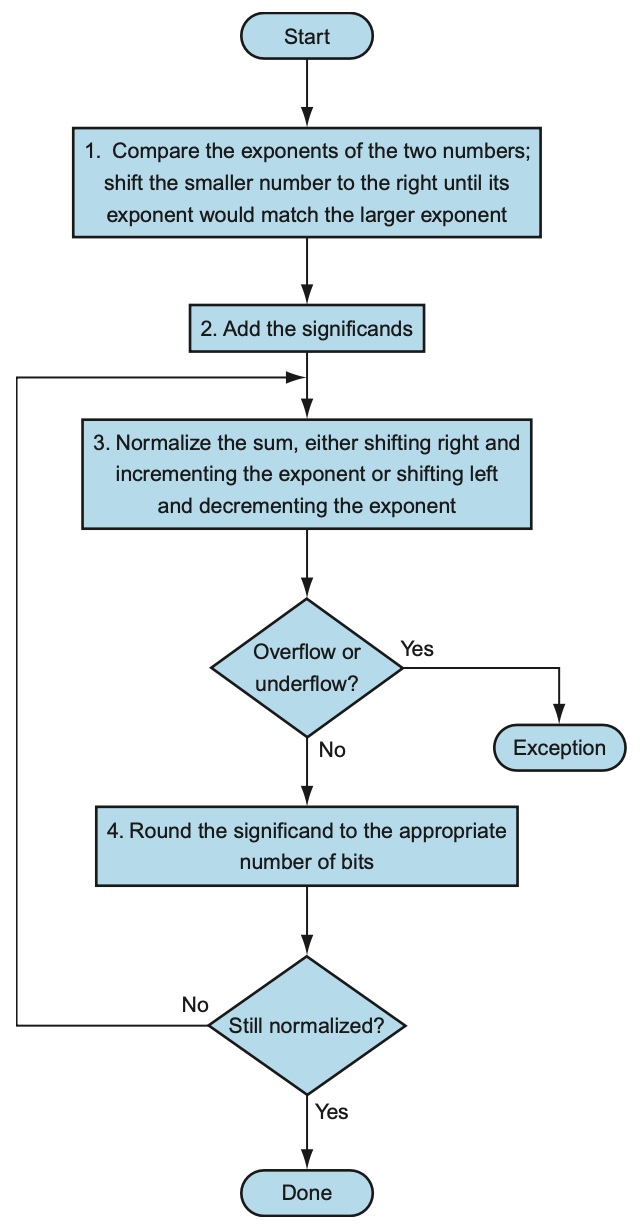
\includegraphics[width=0.32\linewidth]{img/floatingpointadd.png}
    }
    \caption{\textit{Floating-point addition logic path}}
\end{figure}
\pagebreak
\section*{Chapter 1}
\addcontentsline{toc}{section}{Chapter 1}

\subsection*{Design principles}

\subsubsection*{\rightarrow \ \texttt{Design with Moore's Law}}
\vspace{-0.5em}
Moore's Law states that an integrated circuit resources double every 18–24 month.

Thus, computer architects must anticipate where the technology will be when the design finishes rather than design for where it starts.

\subsubsection*{\rightarrow \ \texttt{Abstraction to Simplify Design}}
\vspace{-0.5em}
Abstractions to hide lower-level details to simplify higher-level representations (more productive).

\subsubsection*{\rightarrow \ \texttt{Common case fast}}
\vspace{-0.5em}

If you know what the common case is, enhancing it over the rarer cases is more optimal, as it involves more and is usually easier to enhance.

\subsubsection*{\rightarrow \ \texttt{Performance via Parallelism}}
\vspace{-0.5em}

Computing operations in parallel (at the same time) increases performance over a time period.

\subsubsection*{\rightarrow \ \texttt{Performance via Pipelining}}
\vspace{-0.5em}

Pipelining is a pattern of parallelism that involves increasing the throughput of a certain process (i.e. moving up the chain faster).

\subsubsection*{\rightarrow \ \texttt{Performance via Prediction}}
\vspace{-0.5em}

If you can predict successfully to a degree you can anticipate instead of wait. In some cases it can be more beneficial to guess than to stall when misprediction costs are reasonable.

\subsubsection*{\rightarrow \ \texttt{Memory hierarchy}}
\vspace{-0.5em}

The most expensive and fast memory per bit is at the top, and the opposite is at the bottom. Caches (top) can give the illusion of fast main memory (bottom).

\subsubsection*{\rightarrow \ \texttt{Dependability via Redundancy}}
\vspace{-0.5em}
Systems become dependable when there is redundancy to account for solving failures and failure detections.

\subsection*{Amdahl’s Law}

Related to the design principle of \textit{making the common case fast}, you only benefit from improving the part you actually use, which is illustrated in \textbf{Amdahl's law}.

\begin{tcolorbox}[
    enhanced,
    attach boxed title to top left={xshift=6mm,yshift=-1.5mm},
    colback=moonstoneblue!20,
    colframe=moonstoneblue,
    colbacktitle=moonstoneblue,
    title=Amdahl's Law,
    fonttitle=\bfseries\color{white},
    boxed title style={size=small,colframe=moonstoneblue,sharp corners},
    sharp corners,
    label=box:logic-types,
]
    {\color{moondark}\textbf{Law}}: Performance enhancement possible with a given improvement is limited by the amount that the improved feature is used.
\end{tcolorbox}
\vspace{-2em}
$$S_{\text{total}}\;=\;\frac{1}{(1 - f) + \frac{f}{S_e}}$$

Splitting up the original time into the unimprovable part $1-f$ and the improvable part $f$, speeding up the $f$ portion by $S_E$ yields a time ratio of $$\frac{T_\text{new}}{T_\text{old}}\rightarrow (1-f) + \frac{f}{S_E}$$

As $S_E \rightarrow \infty$, the maximum overall speedup is $\frac{1}{1-f}$.

Thus, taken as the ratio between the old and new speeds, the formula for Amdahl's Law emerges.

\pagebreak

\section*{Chapter 4: Datapath}
\addcontentsline{toc}{section}{Chapter 4: Datapath}

\begin{tcolorbox}[
    enhanced,
    attach boxed title to top left={xshift=6mm,yshift=-1.5mm},
    colback=moonstoneblue!20,
    colframe=moonstoneblue,
    colbacktitle=moonstoneblue,
    title=Logic Design Elements,
    fonttitle=\bfseries\color{white},
    boxed title style={size=small,colframe=moonstoneblue,sharp corners},
    sharp corners,
    label=box:logic-types,
]
    {\color{moondark}\textbf{Combinational elements}}: Do not store any information internally, such as an ALU, and logic gates. \\
    {\color{moondark}\textbf{State elements}}: Have internal memory, a \textit{state}, that remembers even in power loss, such as registers or memory.
\end{tcolorbox}

\subsection*{Branching in the Datapath}

Conditional branching is done by incrementing the PC (program counter, keeps track of the current instruction) by the word (4 bytes) alligned offset (64-bits).

\vspace{-1em}
$$\texttt{B offset \quad \quad CBZ \ Rd, offset}$$

The \texttt{offset} varies in bits by instruction, requiring a sign-extension (from 32 to 64 bits), and 2 left shifts (word aligned multiple of 4 $=2^2$).

\begin{figure}[htbp]
    \centering
    \fcolorbox{codeFrame}{white}{
       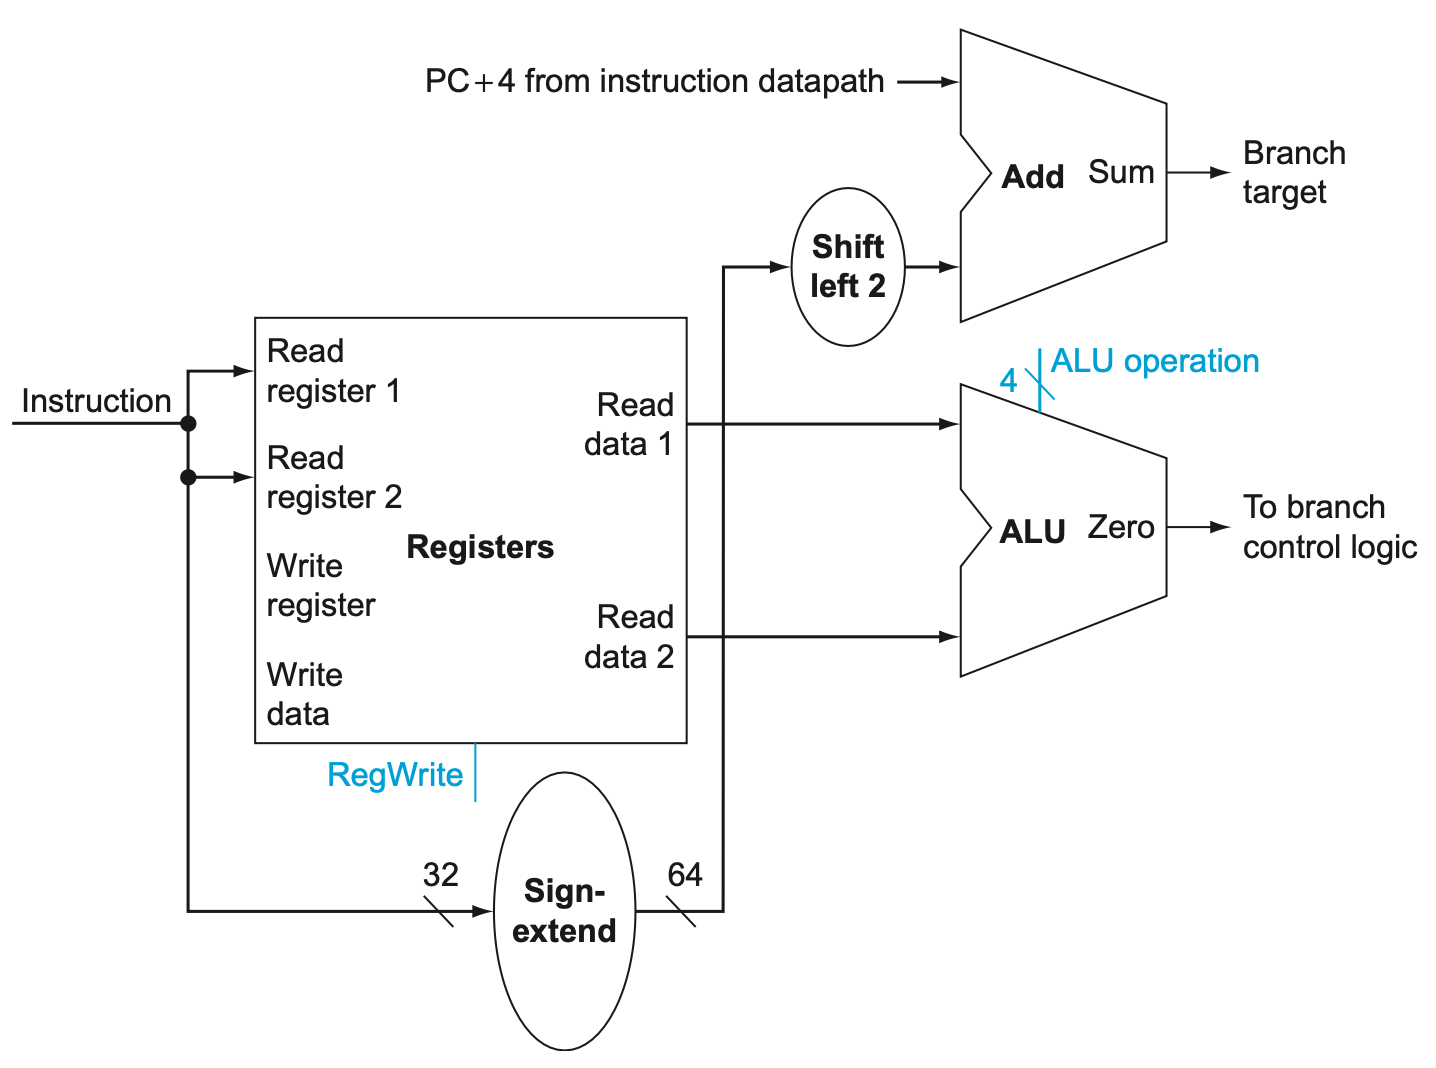
\includegraphics[width=0.5\linewidth]{img/datapath-branch.png}
    }
    \caption{\textit{Subset datapath for unconditional and conditional branching}}
    \label{fig:data-branch}
\end{figure}

Control logic is used to decide whether the incremented PC or branch target should replace the PC, based on the \hyperref[jmp:zero-flag]{zero output} of the ALU, seen in \autoref{fig:data-branch}.


\subsection*{Data memory unit and sign extensions}

The sign extend takes the whole 32-bit instruction and selects the specific offset field size (e.g. 9 bits for loads and stores (small offset needed), 19 bits for \texttt{CBZ}), and fills upper bits with the most significant bit of the extracted address.

\begin{figure}[htbp]
    \centering
    \fcolorbox{codeFrame}{white}{
        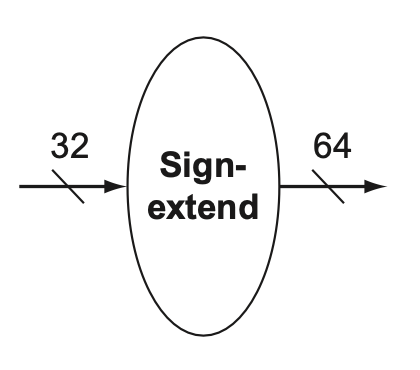
\includegraphics[width=0.2\linewidth]{img/sign-extend.png}
    }
    \caption{\textit{Sign extension from 32 bits to 64 bits}}
\end{figure}


For memory instructions (e.g. \texttt{LDUR}, \texttt{STUR}), we need to write and read from memory using the data memory unit.

The structure takes in the address of memory to access, write input (when storing), read output (when loading), and read and write control signals.

\begin{figure}[htbp]
    \centering
    \fcolorbox{codeFrame}{white}{
       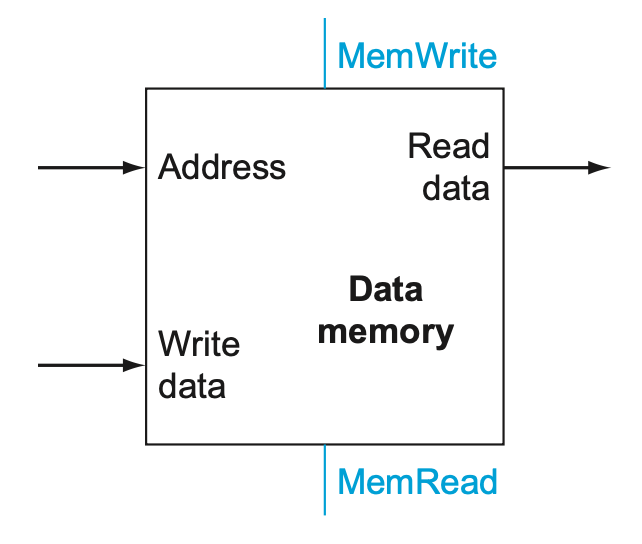
\includegraphics[width=0.3\linewidth]{img/data-memory-unit.png}
    }
    \caption{\textit{Memory data unit diagram}}
\end{figure}

\subsection*{R-type, Branch, and Memory Instruction Datapath}

Building the datapath for R-type (ALU operations), conditional branching, and memory instructions in a \underline{single} clock cycle.

\begin{tcolorbox}[
    enhanced,
    attach boxed title to top left={xshift=6mm,yshift=-1.5mm},
    colback=moonstoneblue!20,
    colframe=moonstoneblue,
    colbacktitle=moonstoneblue,
    title=MUX Controlled by the ALUSrc Signal,
    fonttitle=\bfseries\color{white},
    boxed title style={size=small,colframe=moonstoneblue,sharp corners},
    sharp corners,
    label=box:logic-types,
]
    {\color{moondark}\textbf{R-type}}: Uses the value to do an ALU operation with the first register read output. \\
    {\color{moondark}\textbf{Load/Store (D-type)}}: Uses the sign extended \texttt{offset} with the first output, that holds the memory address to load/store from. In this case, the second read register output is still relevant in storing, as it holds the data to be written.
\end{tcolorbox}

\begin{tcolorbox}[
    enhanced,
    attach boxed title to top left={xshift=6mm,yshift=-1.5mm},
    colback=moonstoneblue!20,
    colframe=moonstoneblue,
    colbacktitle=moonstoneblue,
    title=MUX Controlled by the MemtoReg Signal,
    fonttitle=\bfseries\color{white},
    boxed title style={size=small,colframe=moonstoneblue,sharp corners},
    sharp corners,
    label=box:logic-types,
]
    {\color{moondark}\textbf{R-type}}: Skips the reading stage from the data memory unit and sets the output of the ALU to be the \texttt{Write Data} input of the register file. \\
    {\color{moondark}\textbf{Store (D-type)}}: Reads at \texttt{address + offset} from the data memory unit, and redirects the output to the \texttt{Write Data} input of the register file.
\end{tcolorbox}

\begin{figure}[htbp]
    \centering
    \fcolorbox{codeFrame}{white}{
       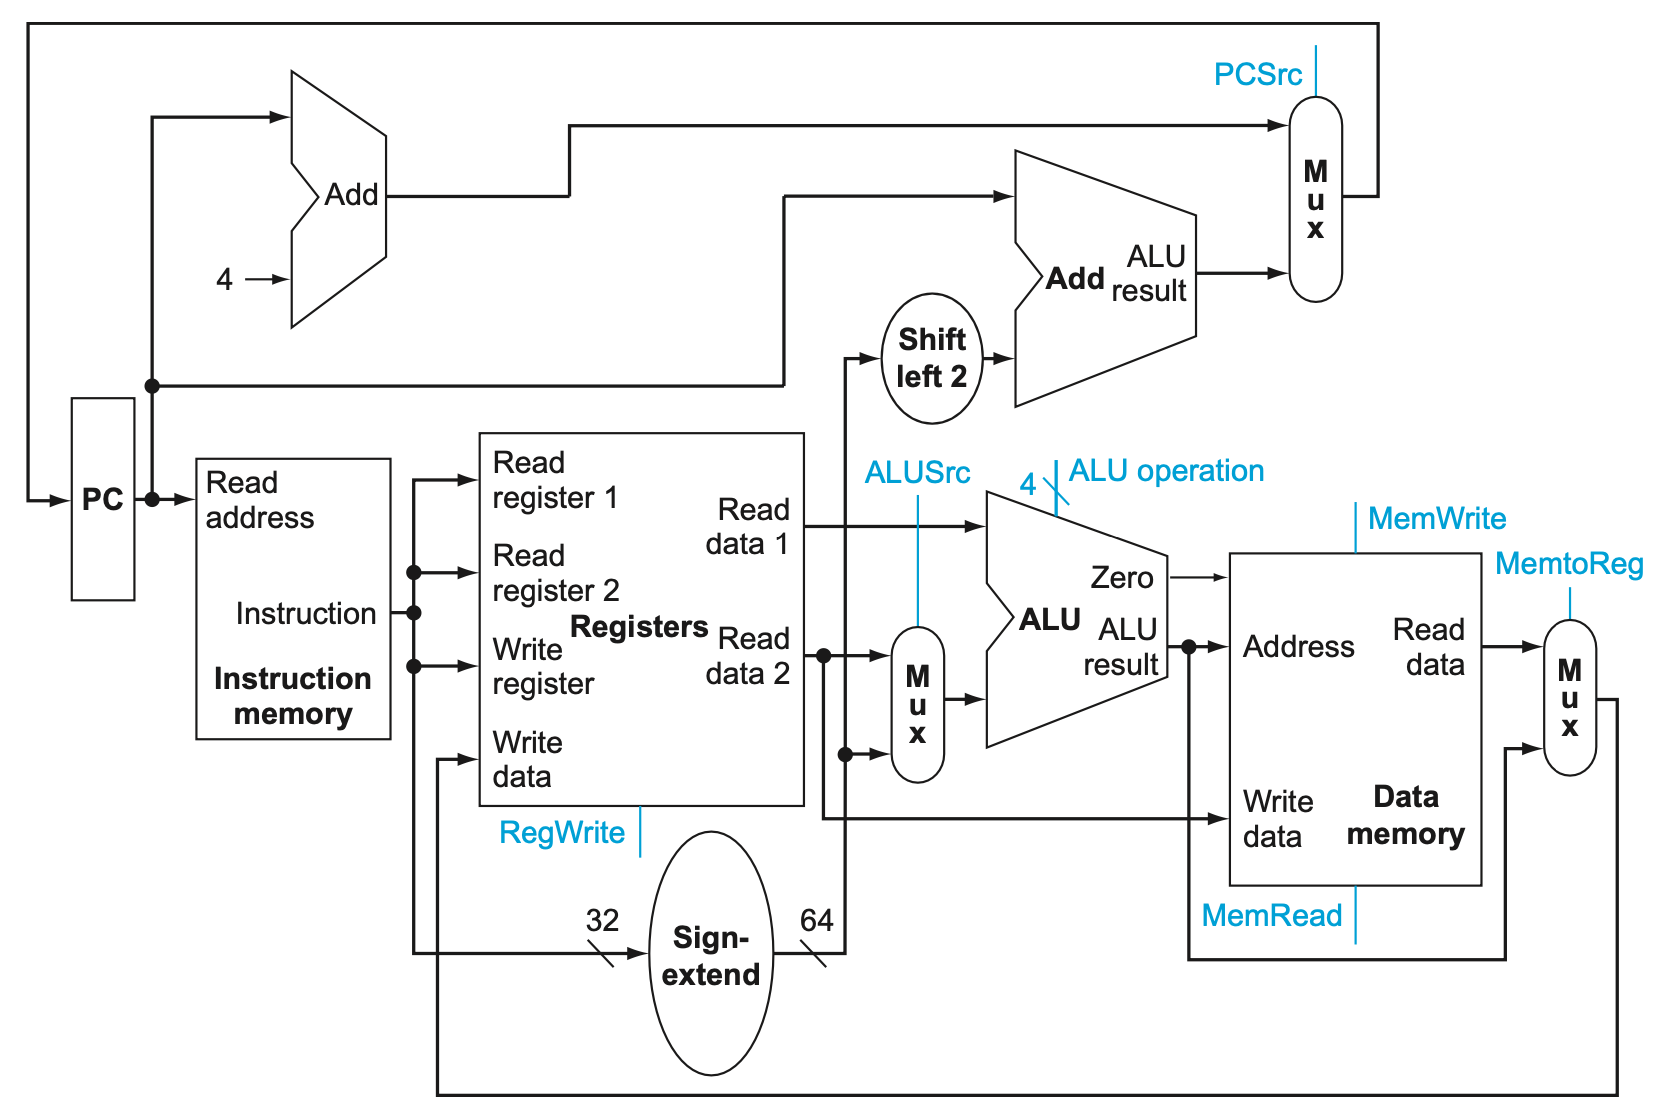
\includegraphics[width=0.8\linewidth]{img/rtype-datapath.png}
    }
    \caption{\textit{Datapath for R-type, load/store, and branching instructions}}
\end{figure}

\subsection*{Instruction Parititions by Instruction Memory}

Considering the R-type, load/store, and conditional branching formats, they are broken down as seen in \autoref{fig:inst-classes}.

\begin{figure}[htbp]
    \centering
    \fcolorbox{codeFrame}{white}{
       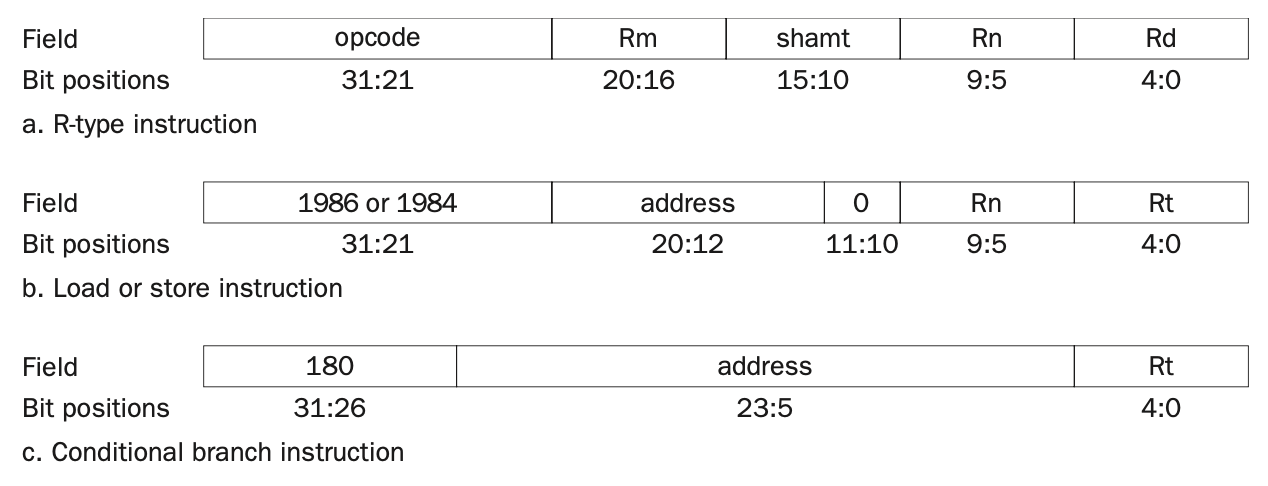
\includegraphics[width=0.55\linewidth]{img/instruction-classes.png}
    }
    \caption{\textit{Memory data unit diagram}}
    \label{fig:inst-classes}
\end{figure}

\textit{Simplicity favors regularity}: The more uniform the design, the simpler the control logic for decoding the instruction (Instruction Memory).

\subsection*{Generating the ALU Control Input}

The ALU control is made up from the \texttt{opcode} (11-bit) and a 2-bit control signal \texttt{ALUOp}.

The \texttt{opcode} field only has three bits that matter when determining function (30, 29, 24).

\texttt{ALUOp} encodes for addition (\texttt{0 0}), passing input B considering \texttt{CBZ} (\texttt{X 1}), and other functions (\texttt{1 X}).
\vspace{-1em}
$$\texttt{ALU operation } (4) = \texttt{ALUOp }(2) + \texttt{opcode } (11 \text{ but uses } 3)$$

\begin{figure}[htbp]
    \centering
    \fcolorbox{codeFrame}{white}{
       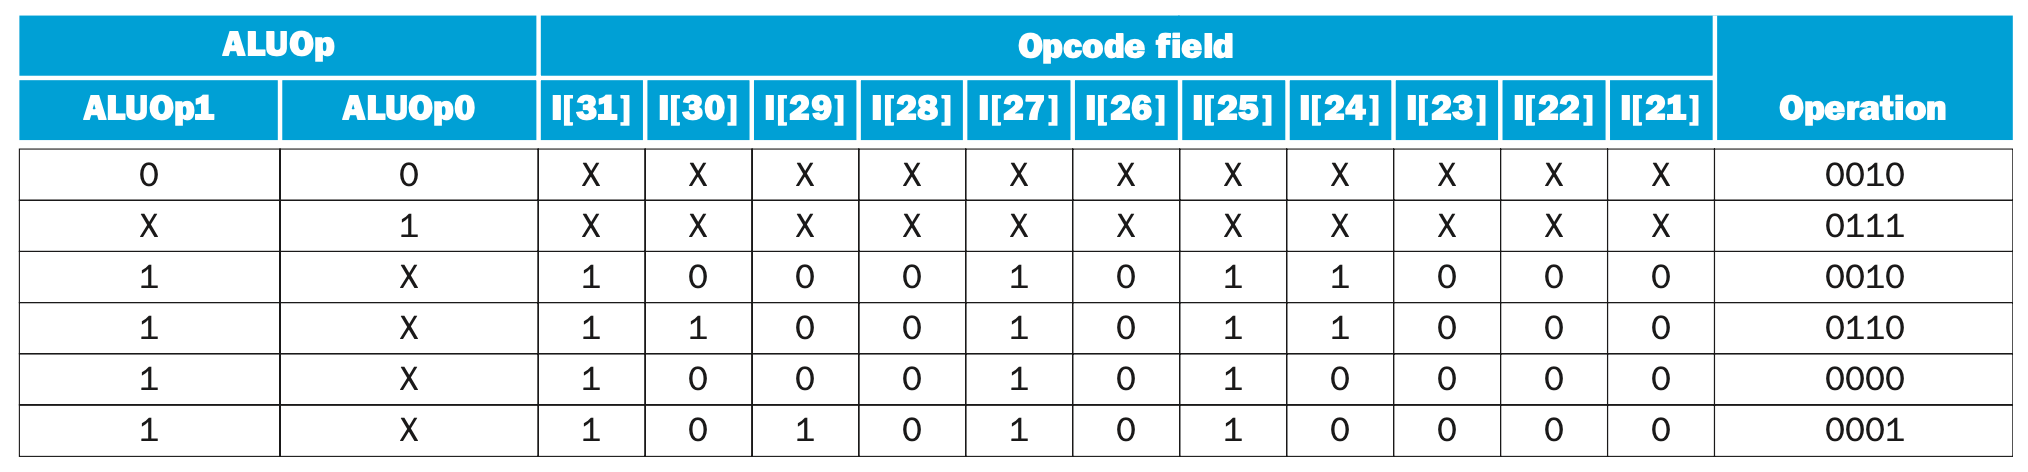
\includegraphics[width=0.7\linewidth]{img/aluop-codes.png}
    }
    \caption{\textit{Truth table for the 4 ALU control bits, with additional "don't care entries"}}
\end{figure}

\begin{figure}[htbp]
    \centering
    \fcolorbox{codeFrame}{white}{
       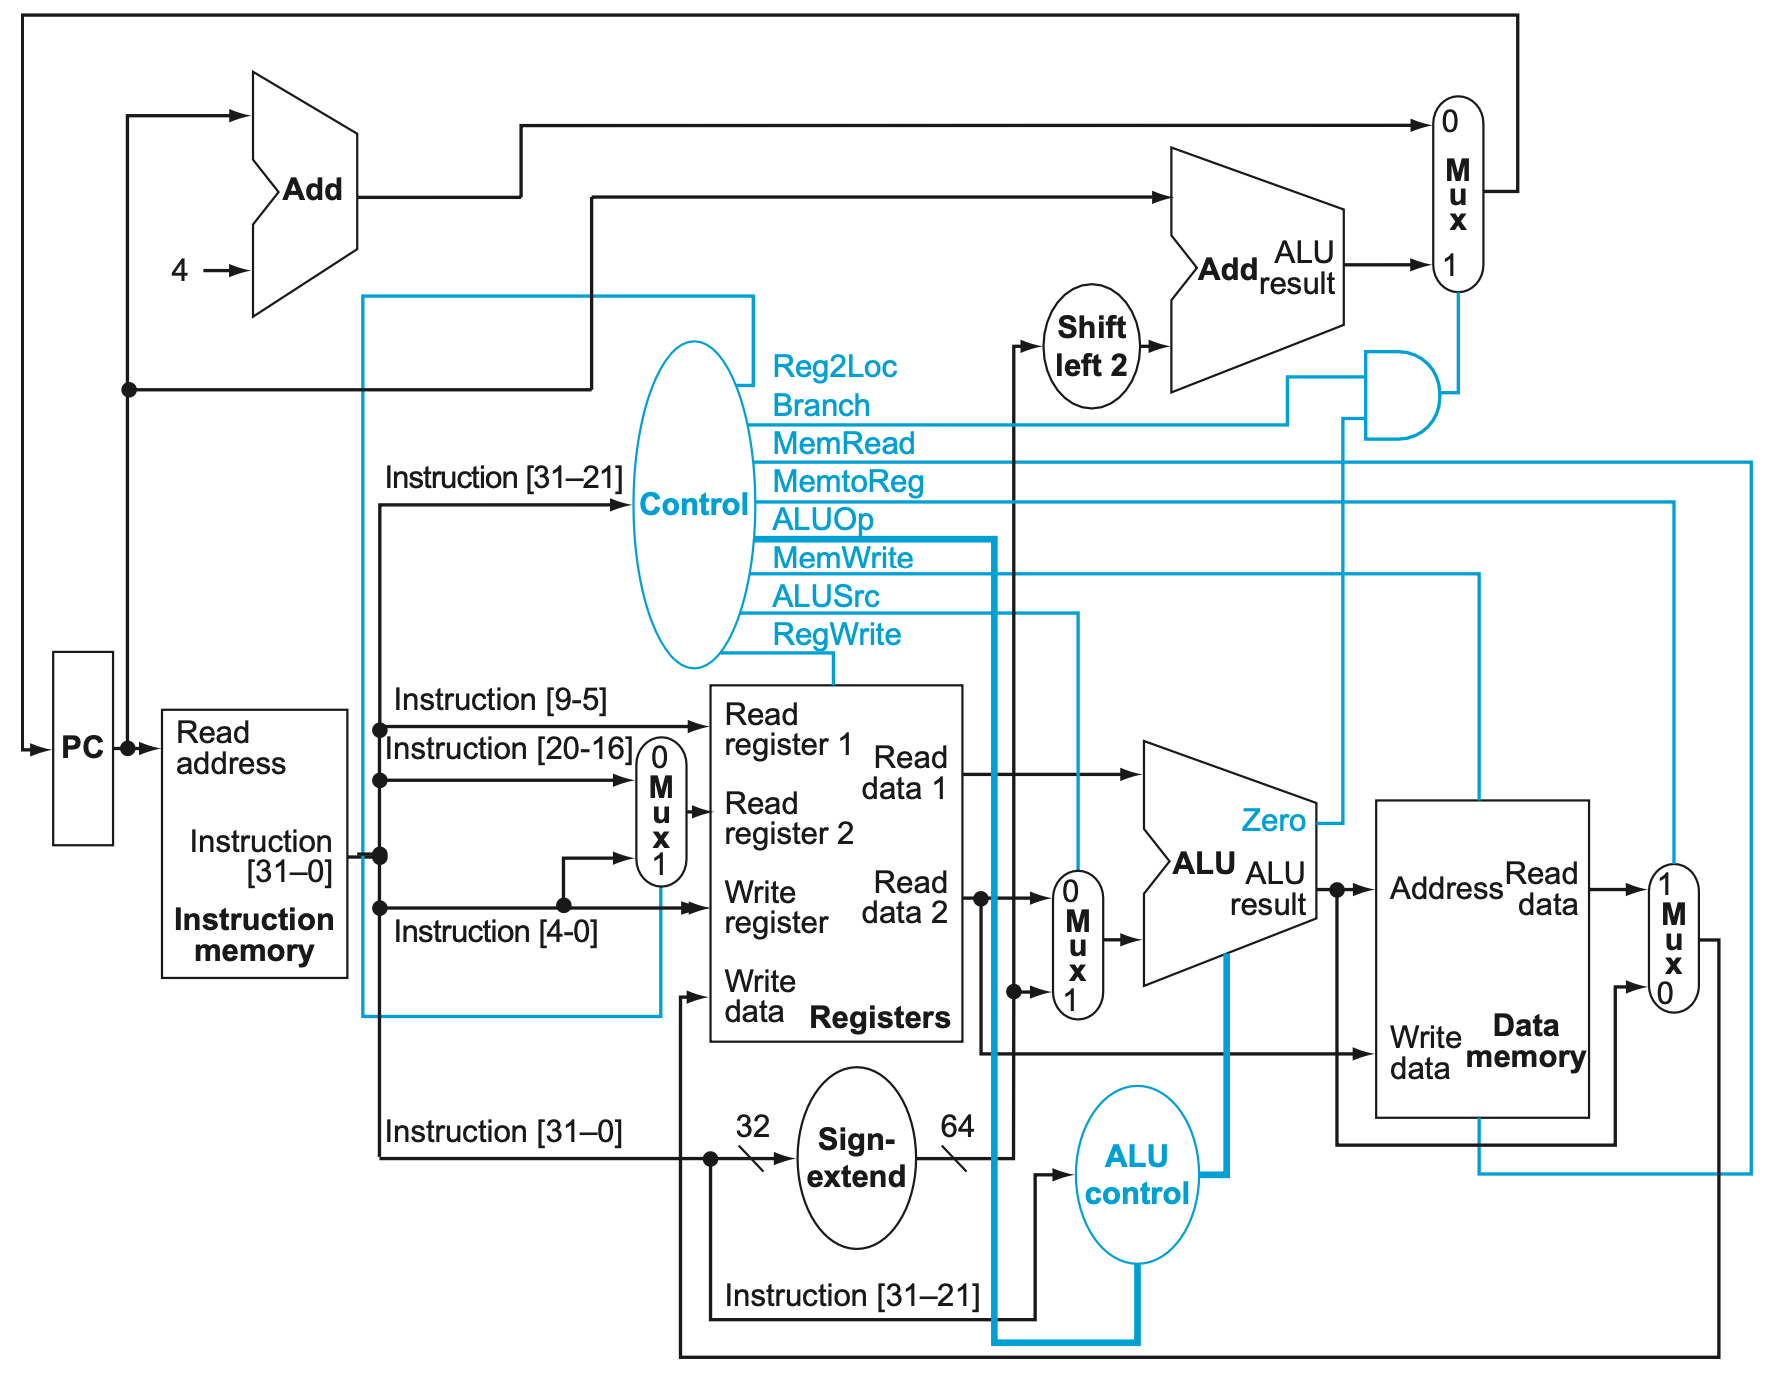
\includegraphics[width=0.7\linewidth]{img/complete-datapath1.png}
    }
    \caption{\textit{Datapath for R-type, D-type, and branching instructions with all 9 control lines}}
    \label{fig:complete-dapath}
\end{figure}

Consider in \autoref{fig:complete-dapath}, the \texttt{PCSrc} signal, that determines whether to increment PC by 4 or by the offset specified, does not originate from the \textbf{control unit}, but rather the \texttt{branch} signal from the control unit being asserted and the zero output of the ALU is asserted.

\begin{figure}[htbp]
    \centering
    \fcolorbox{codeFrame}{white}{
       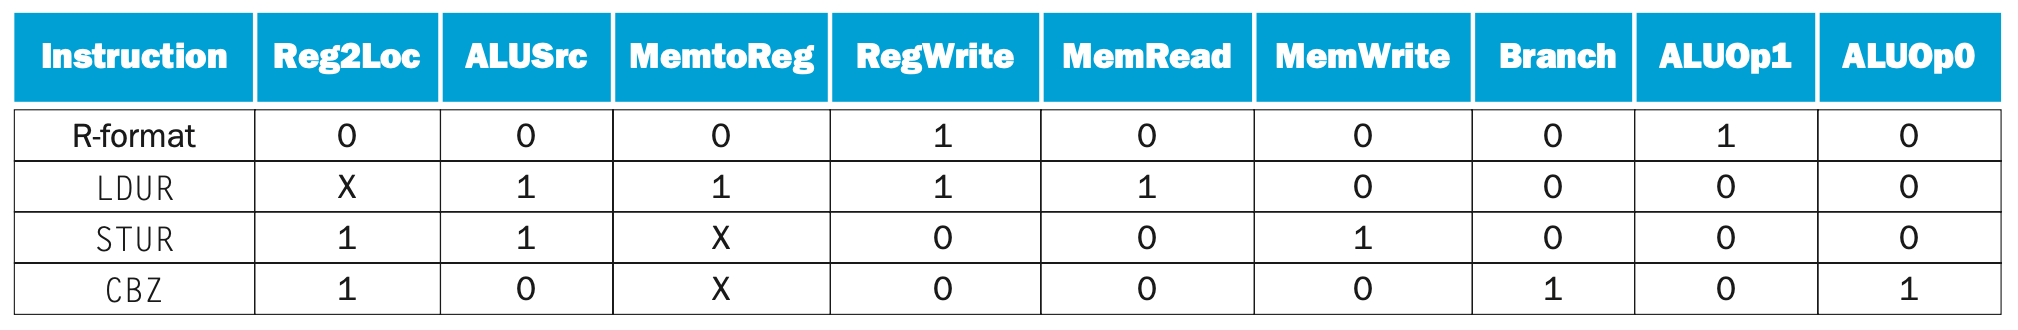
\includegraphics[width=0.7\linewidth]{img/instructions-controllines.png}
    }
    \caption{\textit{Setting control lines according to desired instruction (determined by opcode)}}
\end{figure}

\subsection*{Implementing Unconditional Branching into Datapath}

Adding a new signal \texttt{UncondBranch} to the control unit and \texttt{OR}ing it with the resulting \texttt{PCSrc} control signal that emerges from the \texttt{branch} control signal.

\begin{figure}[htbp]
    \centering
    \fcolorbox{codeFrame}{white}{
       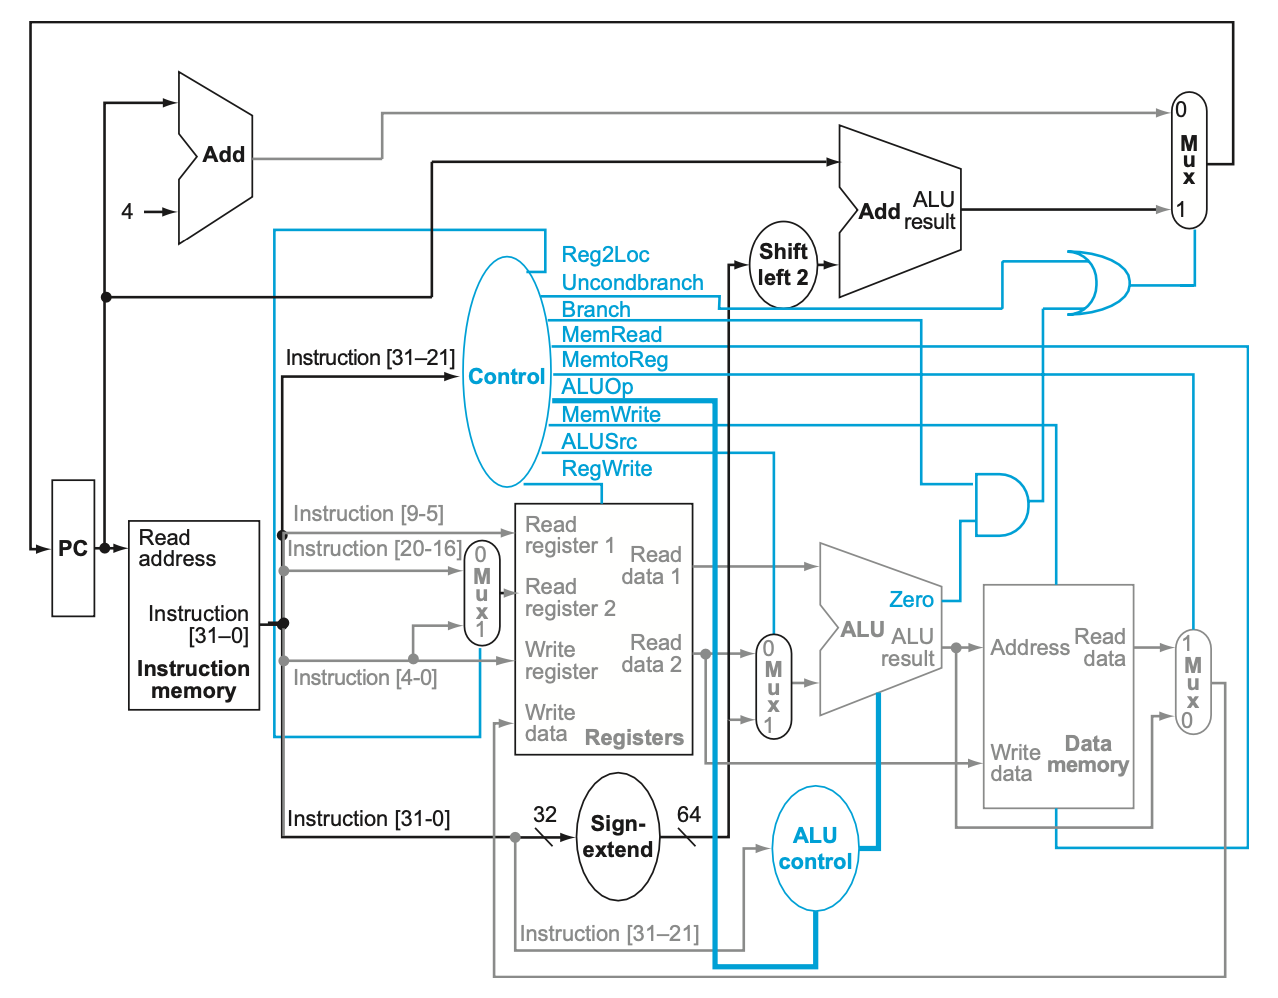
\includegraphics[width=0.7\linewidth]{img/uncond-branch-datapath.png}
    }
    \caption{\textit{Datapath with UncondBranch control signal}}
\end{figure}

Single cycle implementations have the limitation that the clock cycle needs to be greater than the time it takes to complete the longest possible path (load instruction: uses the IM, RegFile, ALU, DataMemory, and the RegFile again).

\pagebreak

\section*{Chapter 4: Pipelining}
\addcontentsline{toc}{section}{Chapter 4: Pipelining}

Pipelining overlaps instructions in execution.

\label{jmp:five-stages}
\begin{tcolorbox}[
    enhanced,
    attach boxed title to top left={xshift=6mm,yshift=-1.5mm},
    colback=moonstoneblue!20,
    colframe=moonstoneblue,
    colbacktitle=moonstoneblue,
    title=LEGv8 Pipelining Steps,
    fonttitle=\bfseries\color{white},
    boxed title style={size=small,colframe=moonstoneblue,sharp corners},
    sharp corners,
    label=box:logic-types,
]
    {\color{moondark}\textbf{1. IF}}: Fetch instructions from memory. \\
    {\color{moondark}\textbf{2. ID}}: Decode instructions and read registers.\\
    {\color{moondark}\textbf{3. EX}}: Executes the op. or calculates the address.\\
    {\color{moondark}\textbf{4. MEM}}: Access data memory (if needed).\\
    {\color{moondark}\textbf{5. WB}}: Writing back into register (if needed).
\end{tcolorbox}

\begin{figure}[htbp]
    \centering
    \fcolorbox{codeFrame}{white}{
       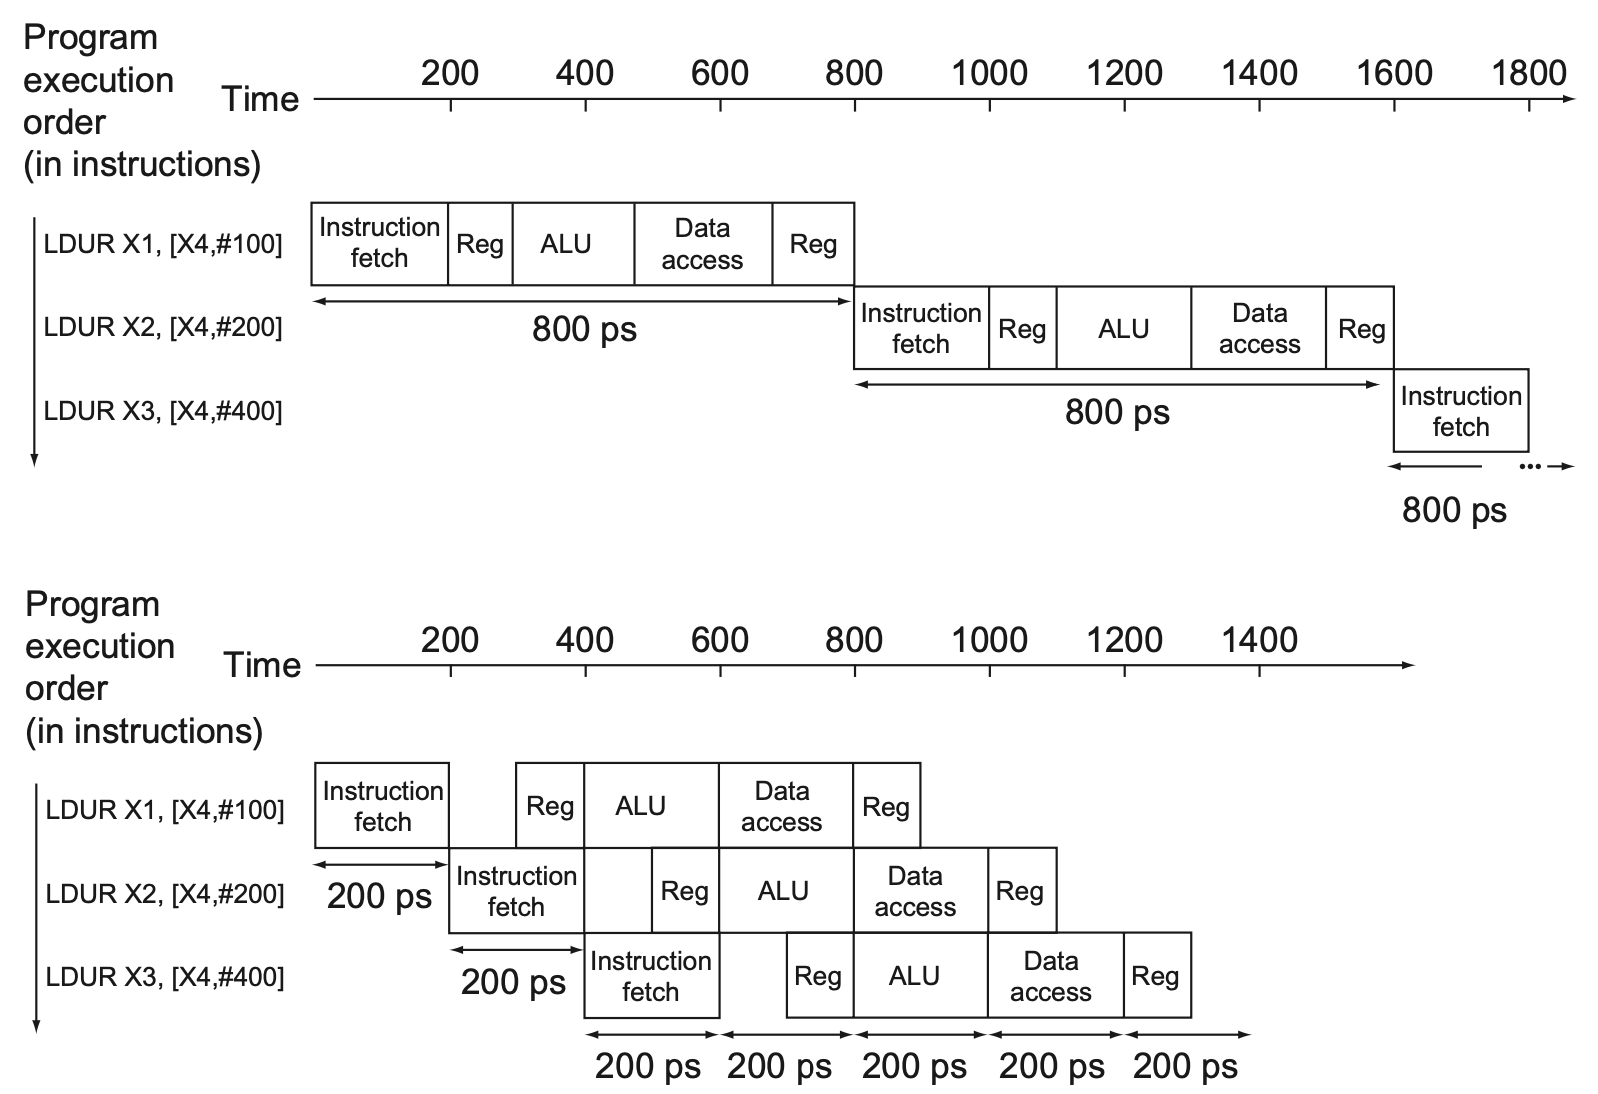
\includegraphics[width=0.7\linewidth]{img/simple-pipeline.png}
    }
    \caption{\textit{Single-cycle execution vs Pipelined execution, showing an improvement from 800ps to 200ps}}
\end{figure}

Pipelining improves performance by increasing instruction \textit{throughput} instead of decreasing execution times by instruction.

\subsection*{Pipelining the Datapath}

The separation of the \hyperref[jmp:five-stages]{five stages} can be seen in the datapath below.

\begin{figure}[htbp]
    \centering
    \fcolorbox{codeframe}{white}{
       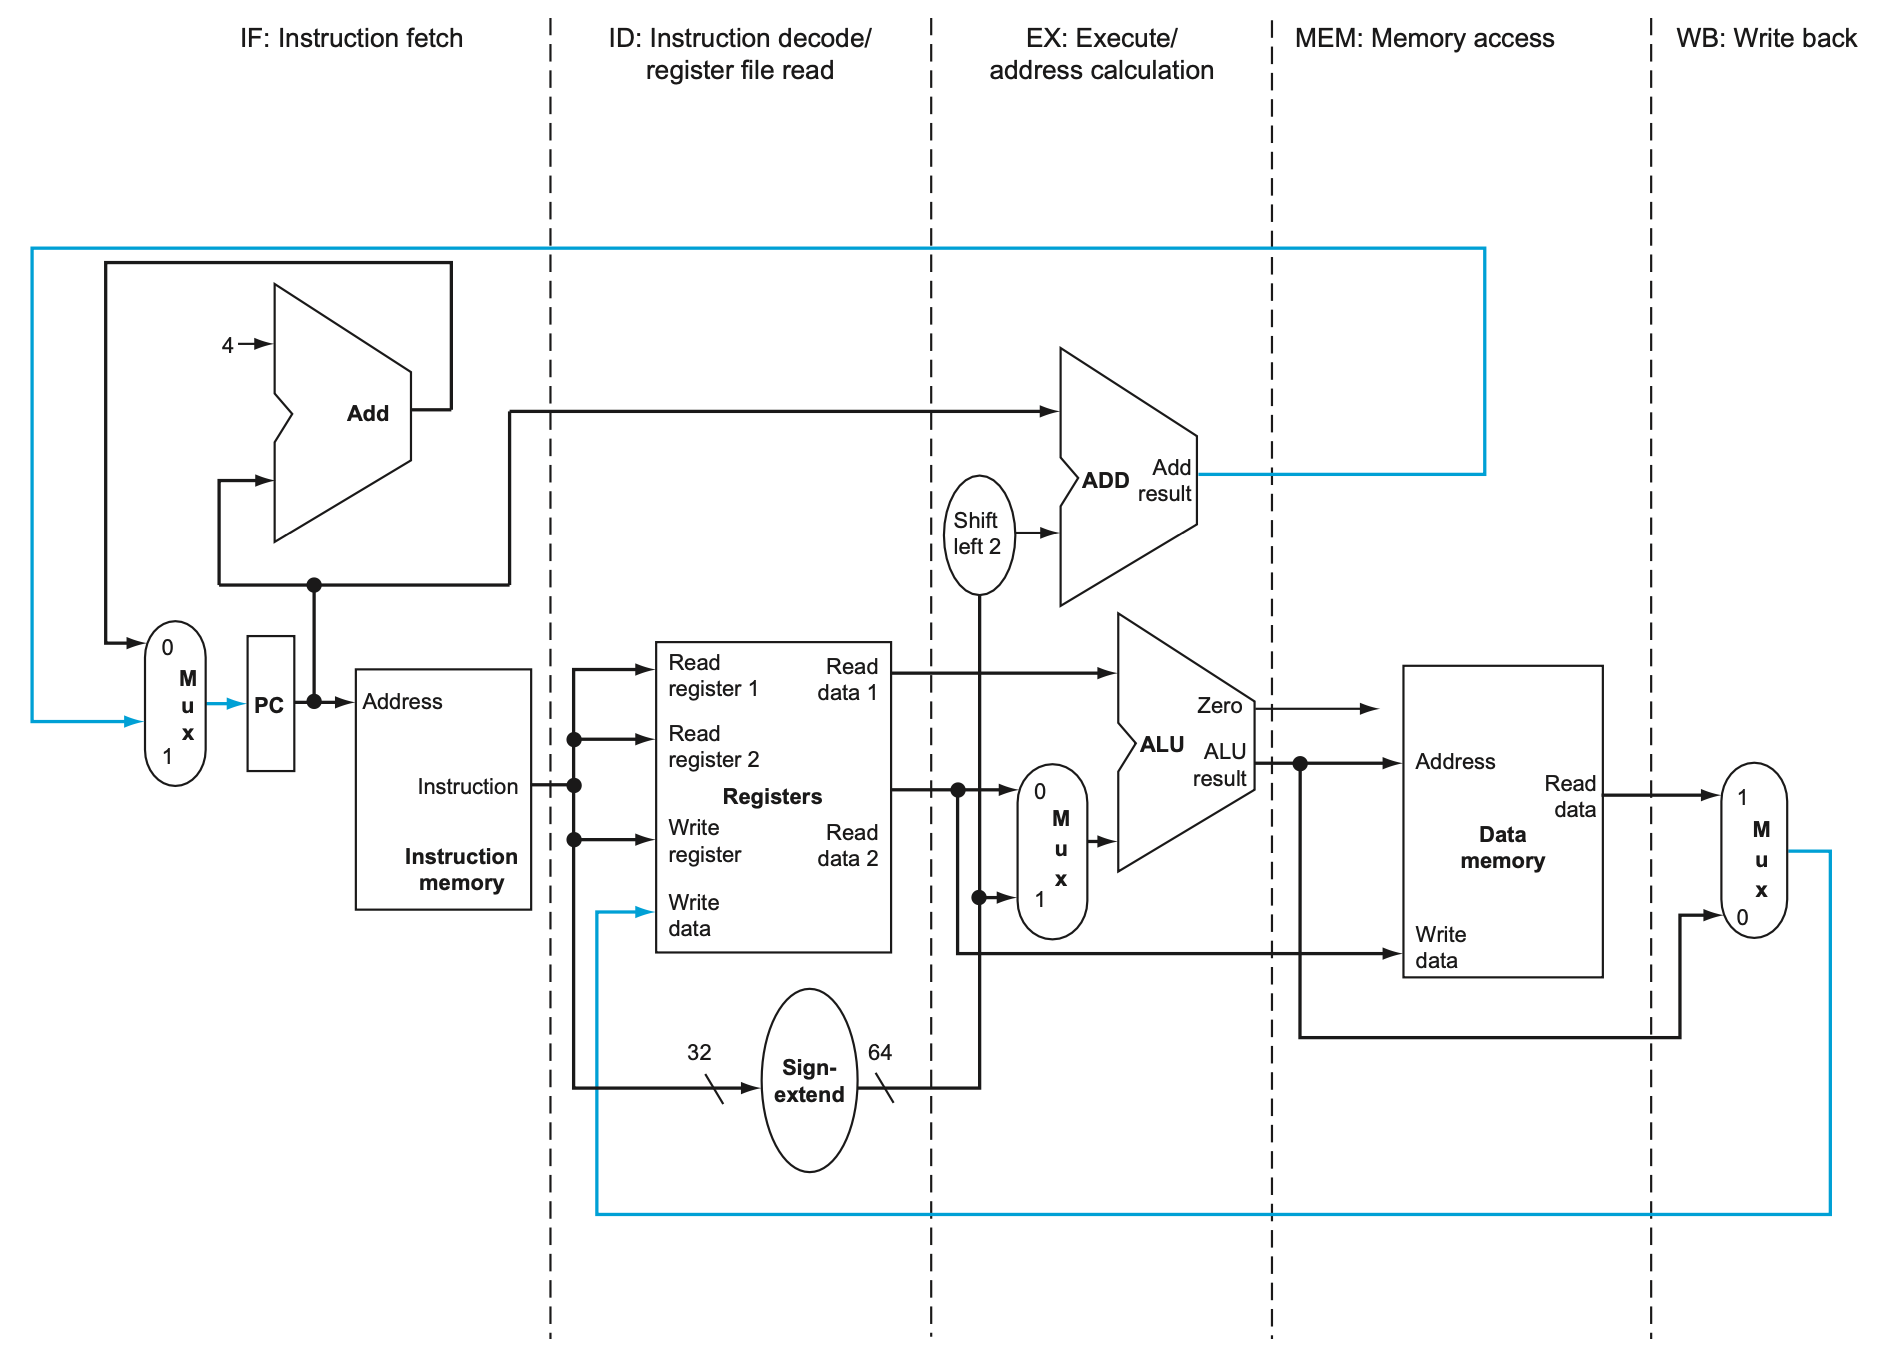
\includegraphics[width=0.7\linewidth]{img/simple-five-stage-datapath.png}
    }
    \caption{\textit{Five stages separation in Datapath}}
\end{figure}

The left to right flow has some exceptions. Write backs involve putting a result in the middle of the path. The selection of the branch that involves +4 or jumping.

Pipeline registers separate the five stages and prevent data loss, keeping stability for newer instructions to use.

\begin{figure}[htbp]
    \centering
    \fcolorbox{codeframe}{white}{
       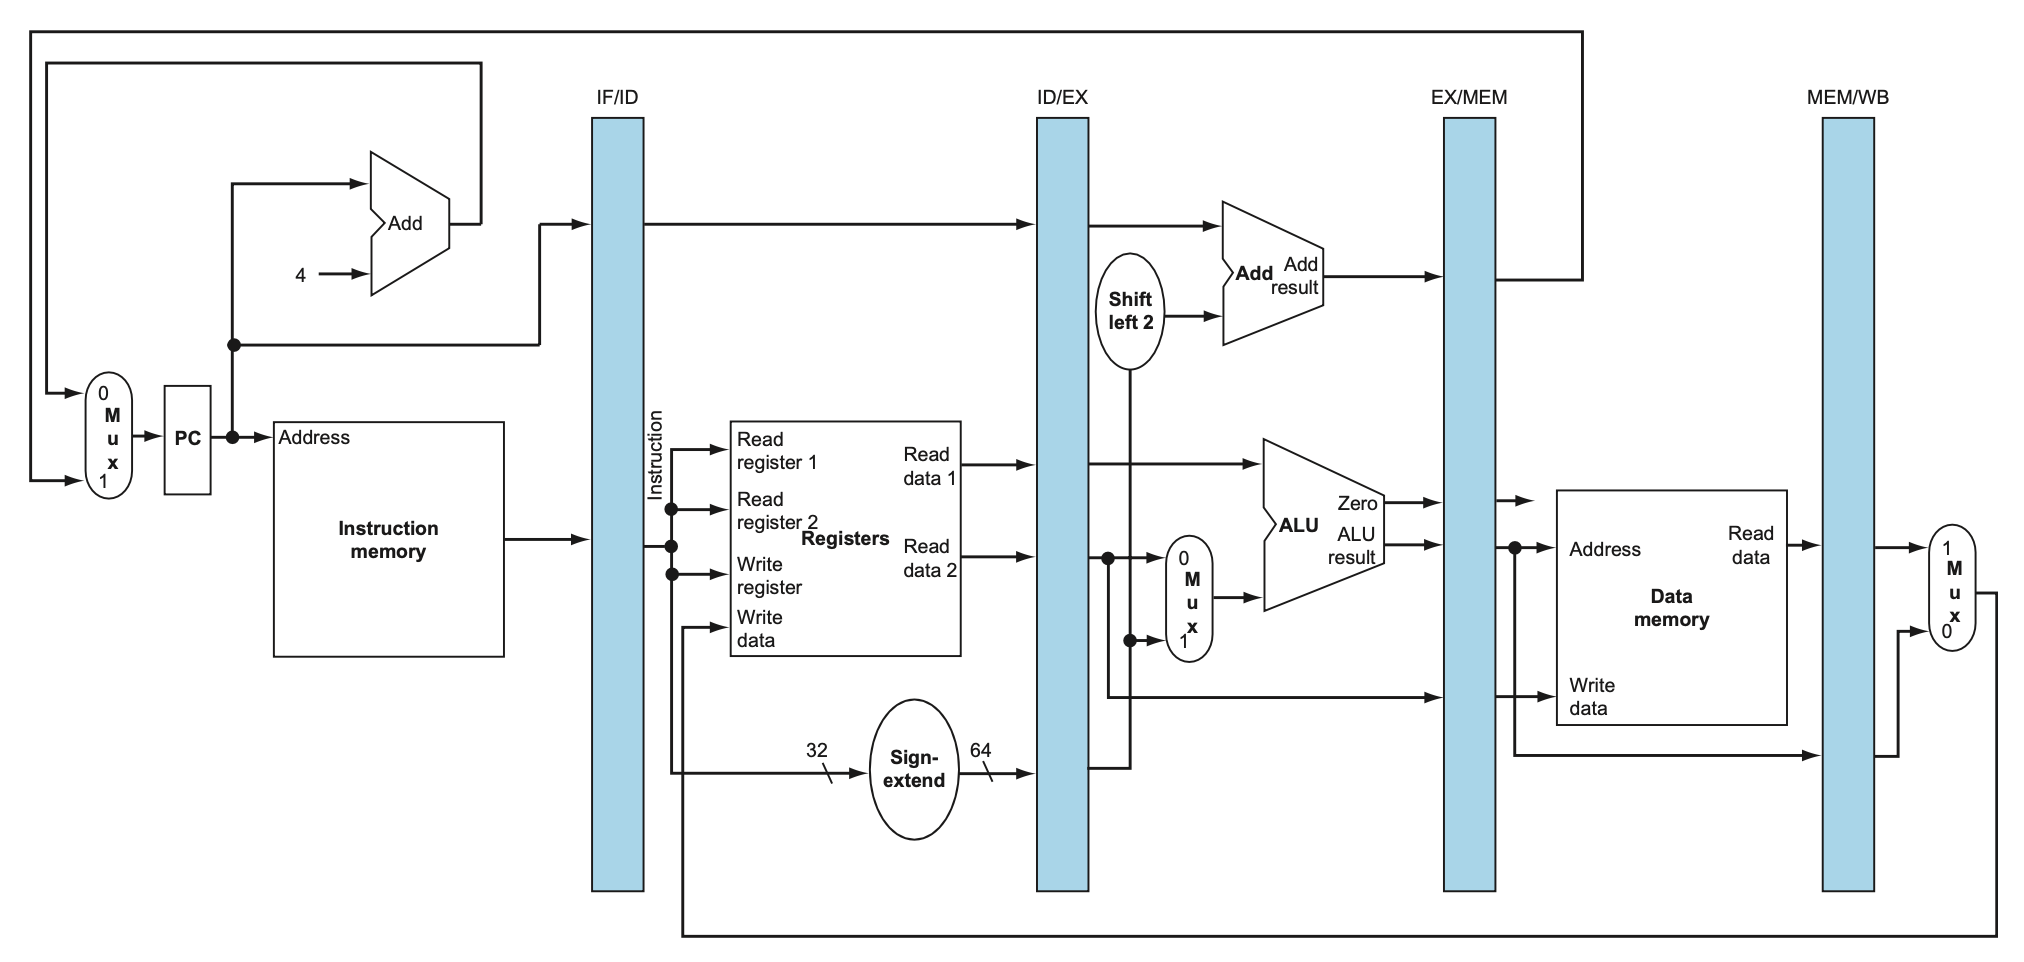
\includegraphics[width=0.7\linewidth]{img/pipelined-reg-datapath.png}
    }
    \caption{\textit{Pipeline registers in Datapath: IF/ID, ID/EX, EX/MEM, MEM/WB}}
\end{figure}

Each logical component (Inst. Mem, RegFile, ALU, etc) must be used only once in a single pipeline stage to avoid \textit{structural hazards}.

As instructions, like loads, need to keep track of a write back register, \texttt{Rt}, which means that this information needs to be propagated all the way upto the MEM/WB stage.

Propagation also happens with the PC, for calculating branching.

\begin{figure}[htbp]
    \centering
    \fcolorbox{codeframe}{white}{
       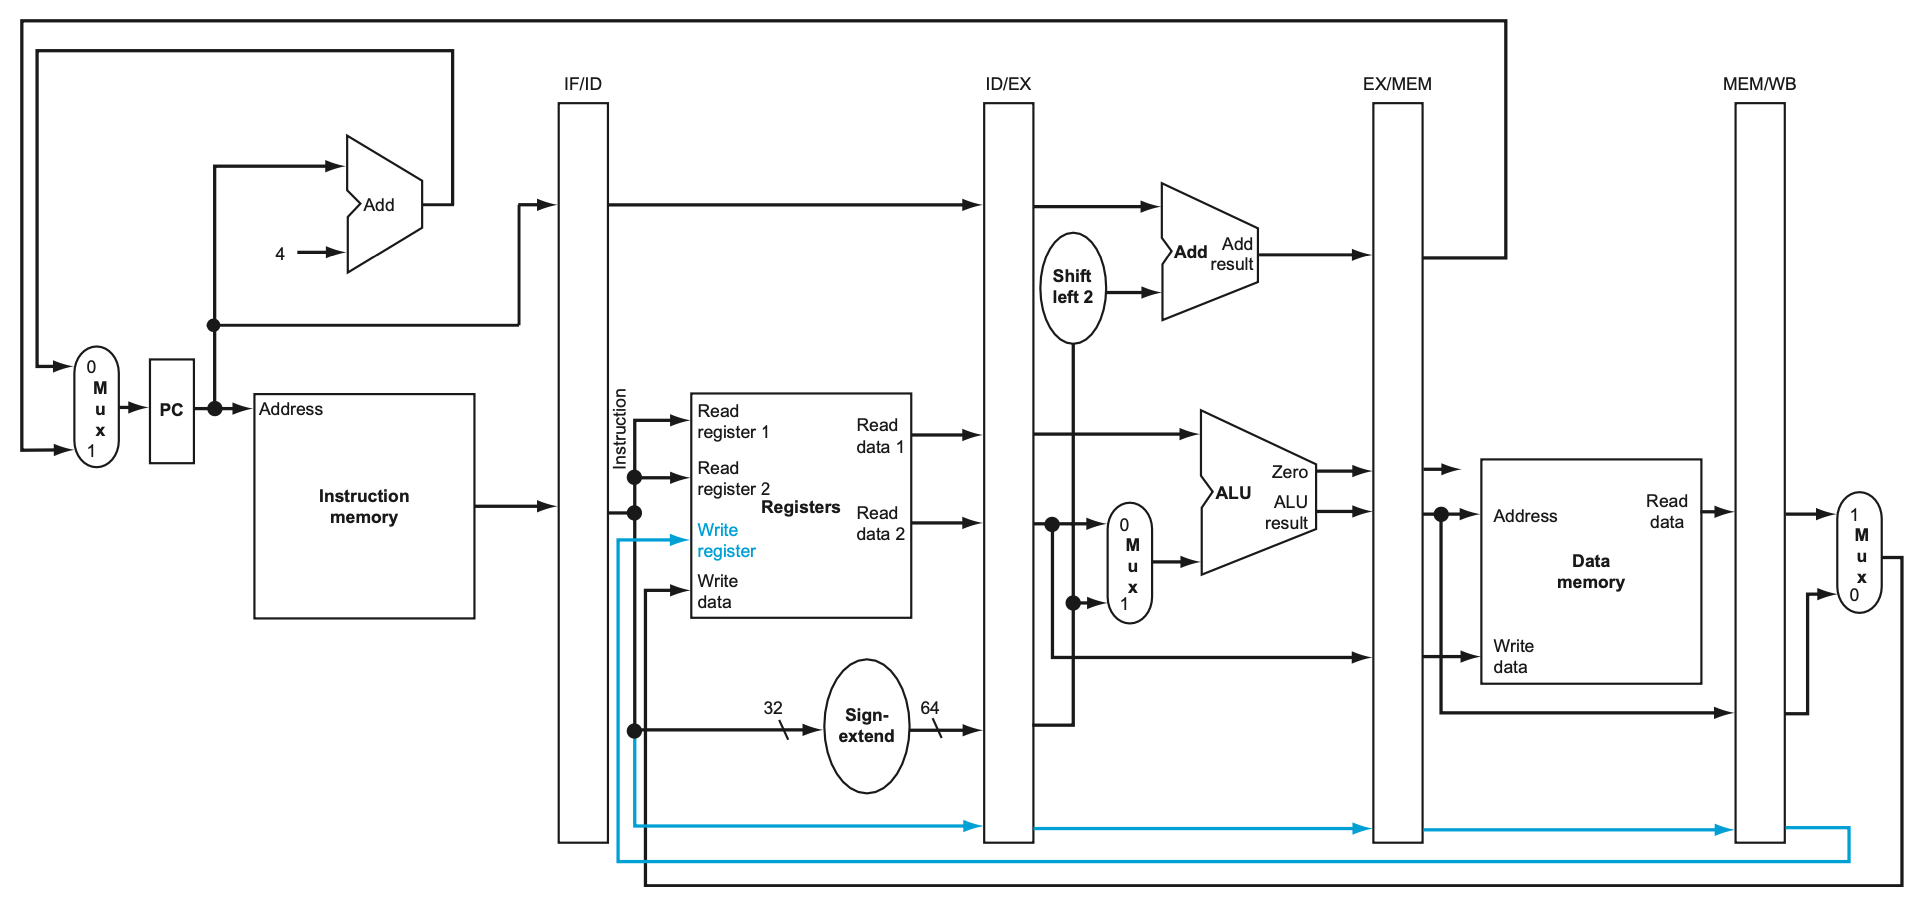
\includegraphics[width=0.7\linewidth]{img/final-pipelined-datapath.png}
    }
    \caption{\textit{Pipelined Datapath with propagates write back register}}
\end{figure}

\subsection*{Pipelining the Control}

As each control line is associated with one component active in one pipeline stage, the five stages can be used to classify the existing control signals. This means that pipelined registers can be expanded to fit the control signals.

\begin{figure}[htbp]
    \centering
    \fcolorbox{codeframe}{white}{
       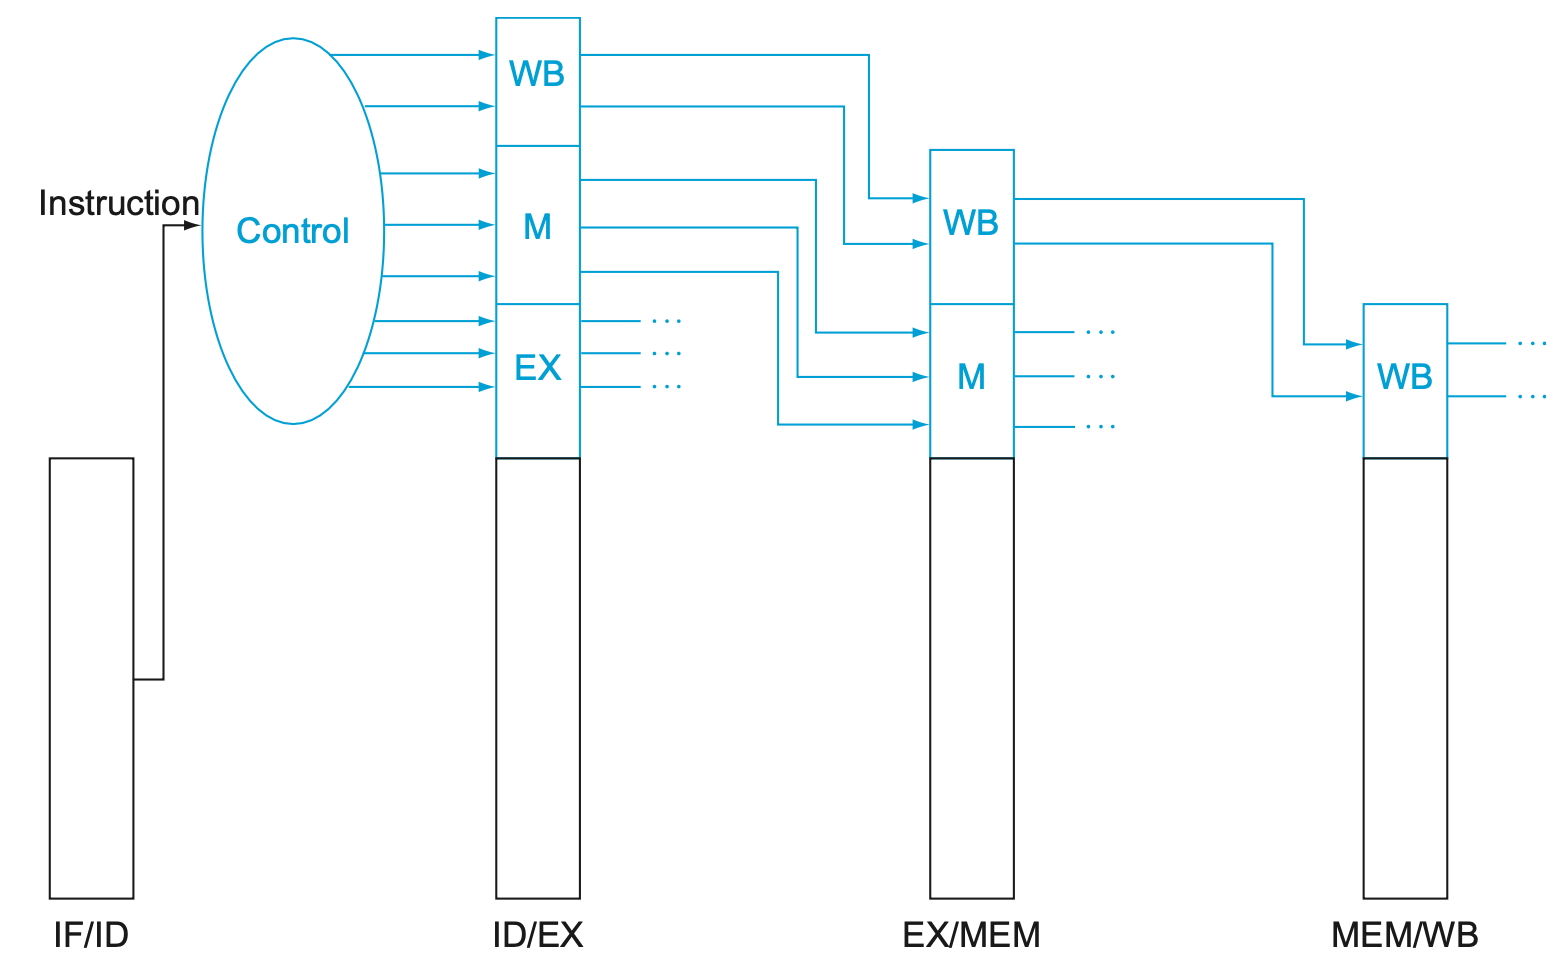
\includegraphics[width=0.7\linewidth]{img/control-piped.png}
    }
    \caption{\textit{Control signals with applied Pipelining}}
\end{figure}

Considering that the control signals start at EX, the control information can be created at ID.

\begin{figure}[htbp]
    \centering
    \fcolorbox{codeframe}{white}{
       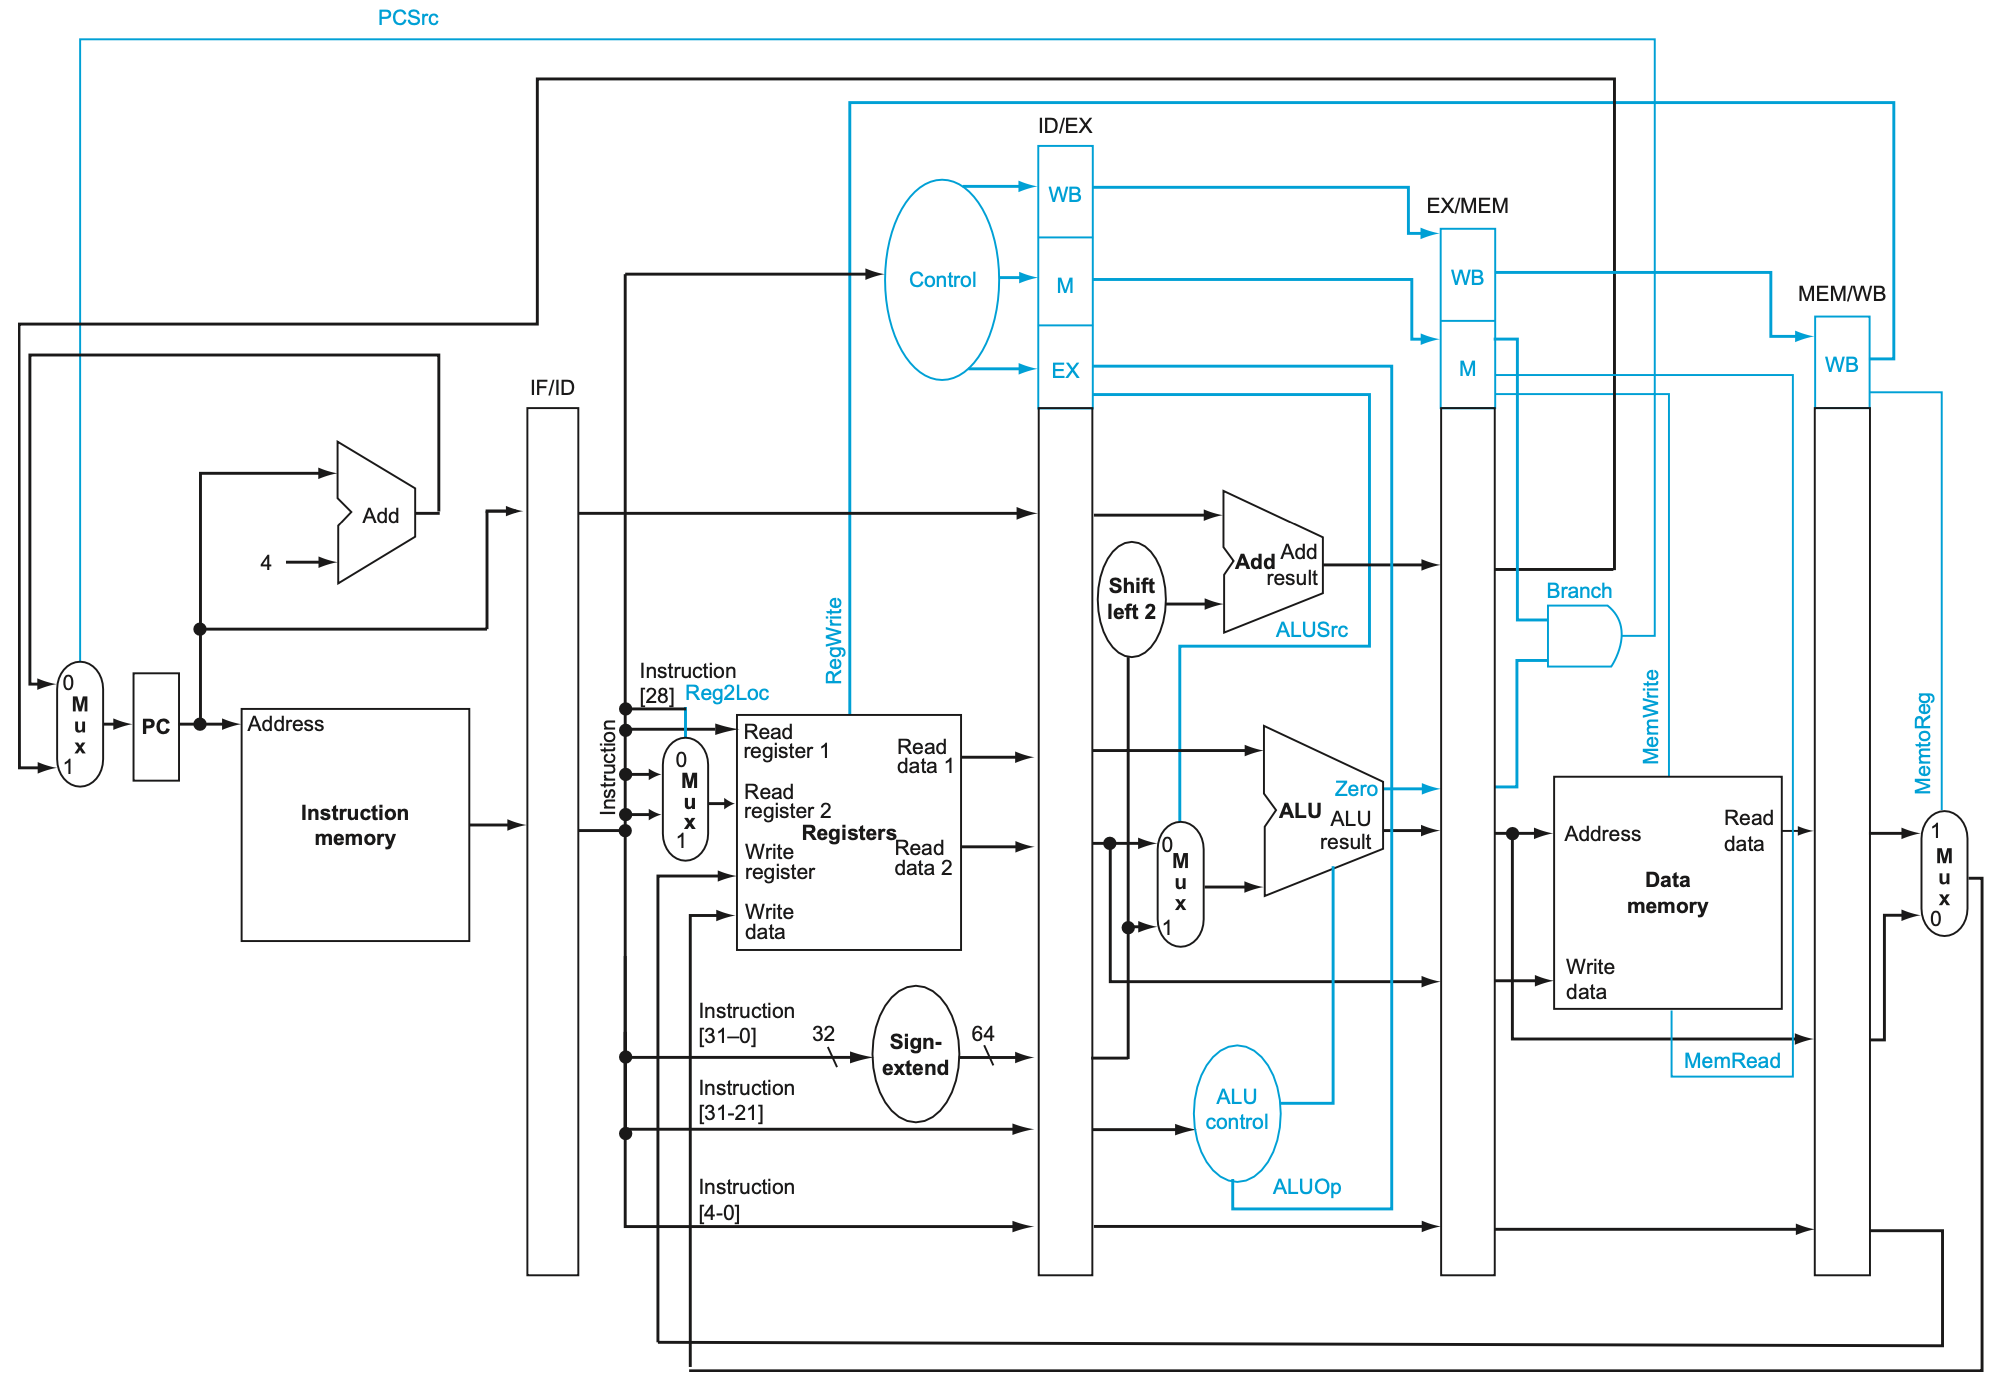
\includegraphics[width=0.7\linewidth]{img/full-control-pipeline.png}
    }
    \caption{\textit{Pipelined Datapath with Pipelined Control Signals}}
\end{figure}

The \texttt{Reg2Loc} signal is directly encoded into the instruction field as a bit that determined whether to use the \texttt{Rm} for R-type or \texttt{Rt} for cond. branching and load/store instructions.

\subsection*{Pipeline Hazards}

\subsubsection*{\rightarrow \ \texttt{Structural Hazard}}
\vspace{-0.5em}

When one element cannot support two instructions at the same time.

Imagined if there was no distinction between IM and Data Memory, which would cause a first instruction to access data, while a fourth one is trying to fetch it at the same time.

\subsubsection*{\rightarrow \ \texttt{Data Hazards}}
\vspace{-0.5em}

When a new instruction needs data from another instruction that has not yet finished executing.

Data dependence from one instruction to an earlier one.

\begin{verbatim}
    ADD     X19, X0, X1
    SUB     X2, X19, X3     // X19 depends on ADD instruction's execution
\end{verbatim}

Stalling would cause a waste of 3 clock cycles, and compilers opts are not enough.

A solution is to \textbf{forward} or bypass, which entails, in the example, to supply the result of the ALU directly into the input of the subtraction (or RegFile write).

\begin{figure}[htbp]
    \centering
    \fcolorbox{codeframe}{white}{
       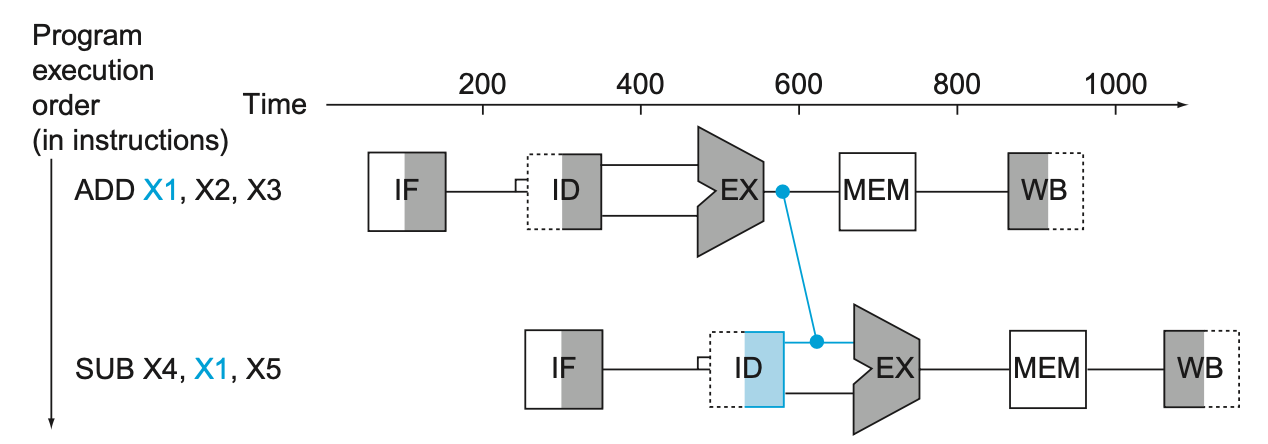
\includegraphics[width=0.7\linewidth]{img/simple-forwarding.png}
    }
    \caption{\textit{forwarding implementation in \texttt{ADD} and \texttt{SUB} example}}
\end{figure}

There are cases where pipeline stalls or bubbles are present in forwarding, such as the \textbf{load-use data hazard}, in which the data has not yet been loaded when they are needed by another instruction.

\pagebreak
\begin{figure}[htbp]
    \centering
    \fcolorbox{codeframe}{white}{
       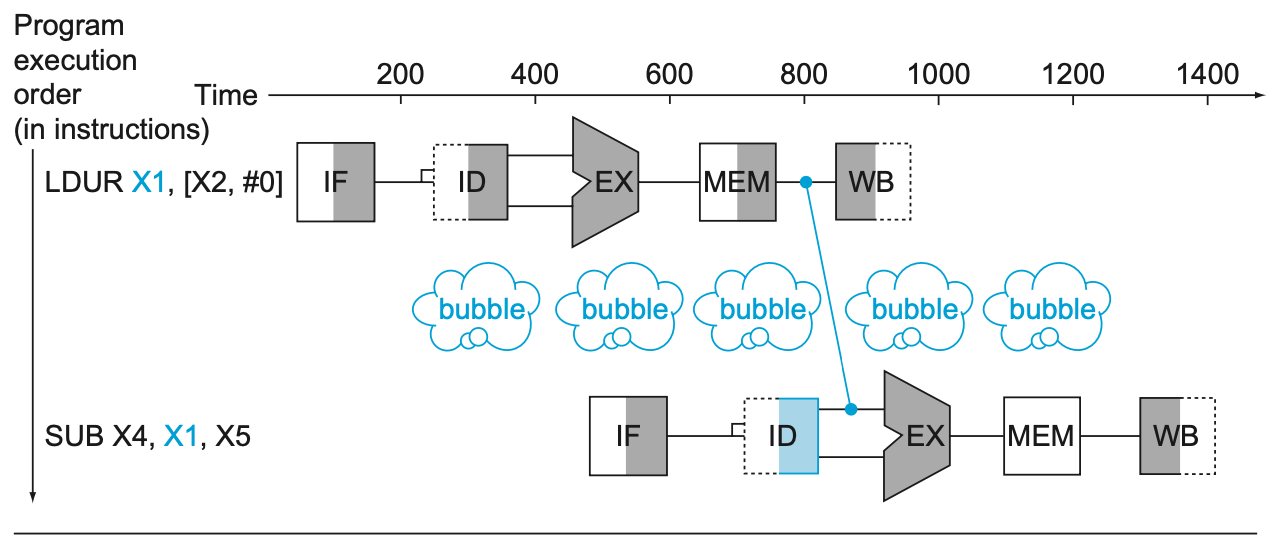
\includegraphics[width=0.7\linewidth]{img/load-after-use-stall.png}
    }
    \caption{\textit{Load-use hazard with one cycle stalling to forward data}}
\end{figure}

\textbf{True data dependences} are when results are used later as operands.

\textbf{False data dependences} are when results are not passed through yet are clobbered, such as reading a register and then writing to the same register (write clobbers the read, but can be solved by using another register name).

\begin{tcolorbox}[
    enhanced,
    attach boxed title to top left={xshift=6mm,yshift=-1.5mm},
    colback=moonstoneblue!20,
    colframe=moonstoneblue,
    colbacktitle=moonstoneblue,
    title=Types of False Data Dependences,
    fonttitle=\bfseries\color{white},
    boxed title style={size=small,colframe=moonstoneblue,sharp corners},
    sharp corners,
    label=box:logic-types,
]
    {\color{moondark}\textbf{Anti-dependence}}: Reading a register and then writting (clobbering) to the same register (WAR). \\
    {\color{moondark}\textbf{Output dependence}}: Writing to a register and then writing to the same register (WAW).
\end{tcolorbox}

\pagebreak
\begin{figure}[htbp]
    \centering
    \fcolorbox{codeframe}{white}{
       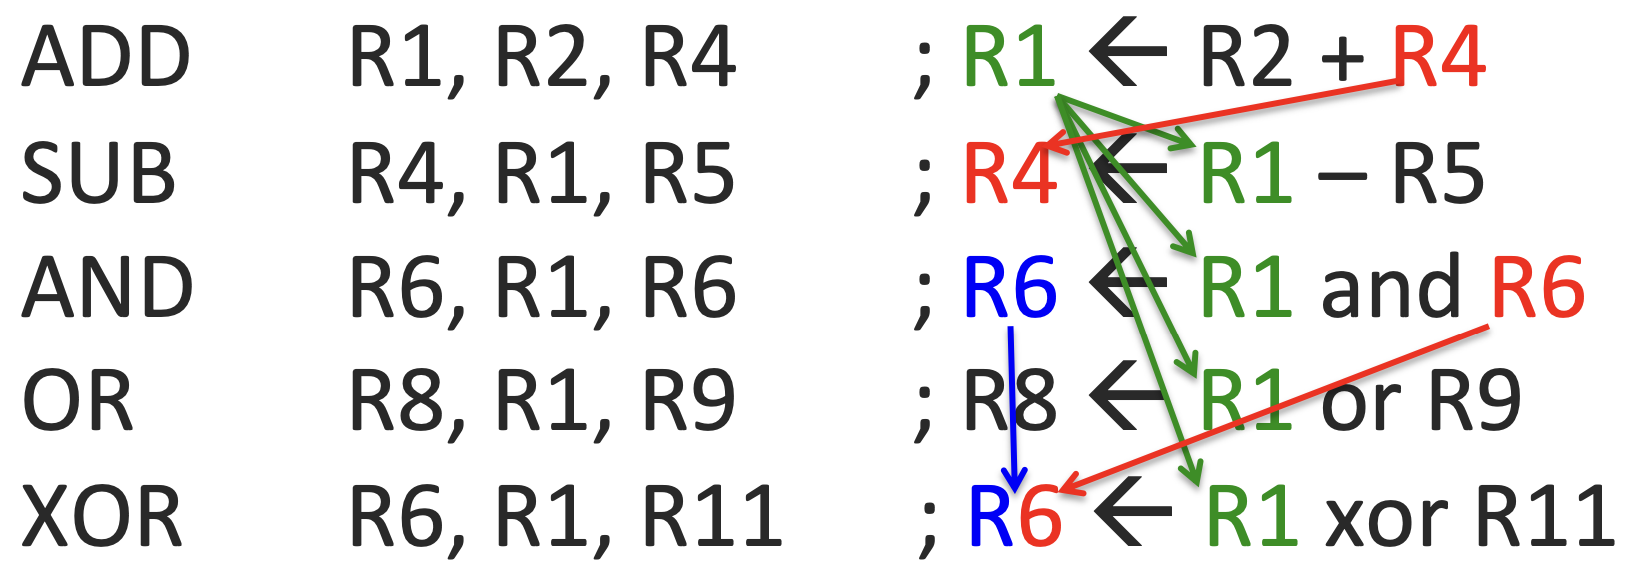
\includegraphics[width=0.5\linewidth]{img/datadep-example.png}
    }
    \caption{\textit{Green are True dependences, Red are Anti-dependences, and Blue are Output-dependences}}
\end{figure}

For stalling you can use \texttt{NOP} instructions that have no effect other than acting as bubbles in the pipeline, in order to conserve the forwarding.

\begin{figure}[htbp]
    \centering
    \fcolorbox{codeframe}{white}{
       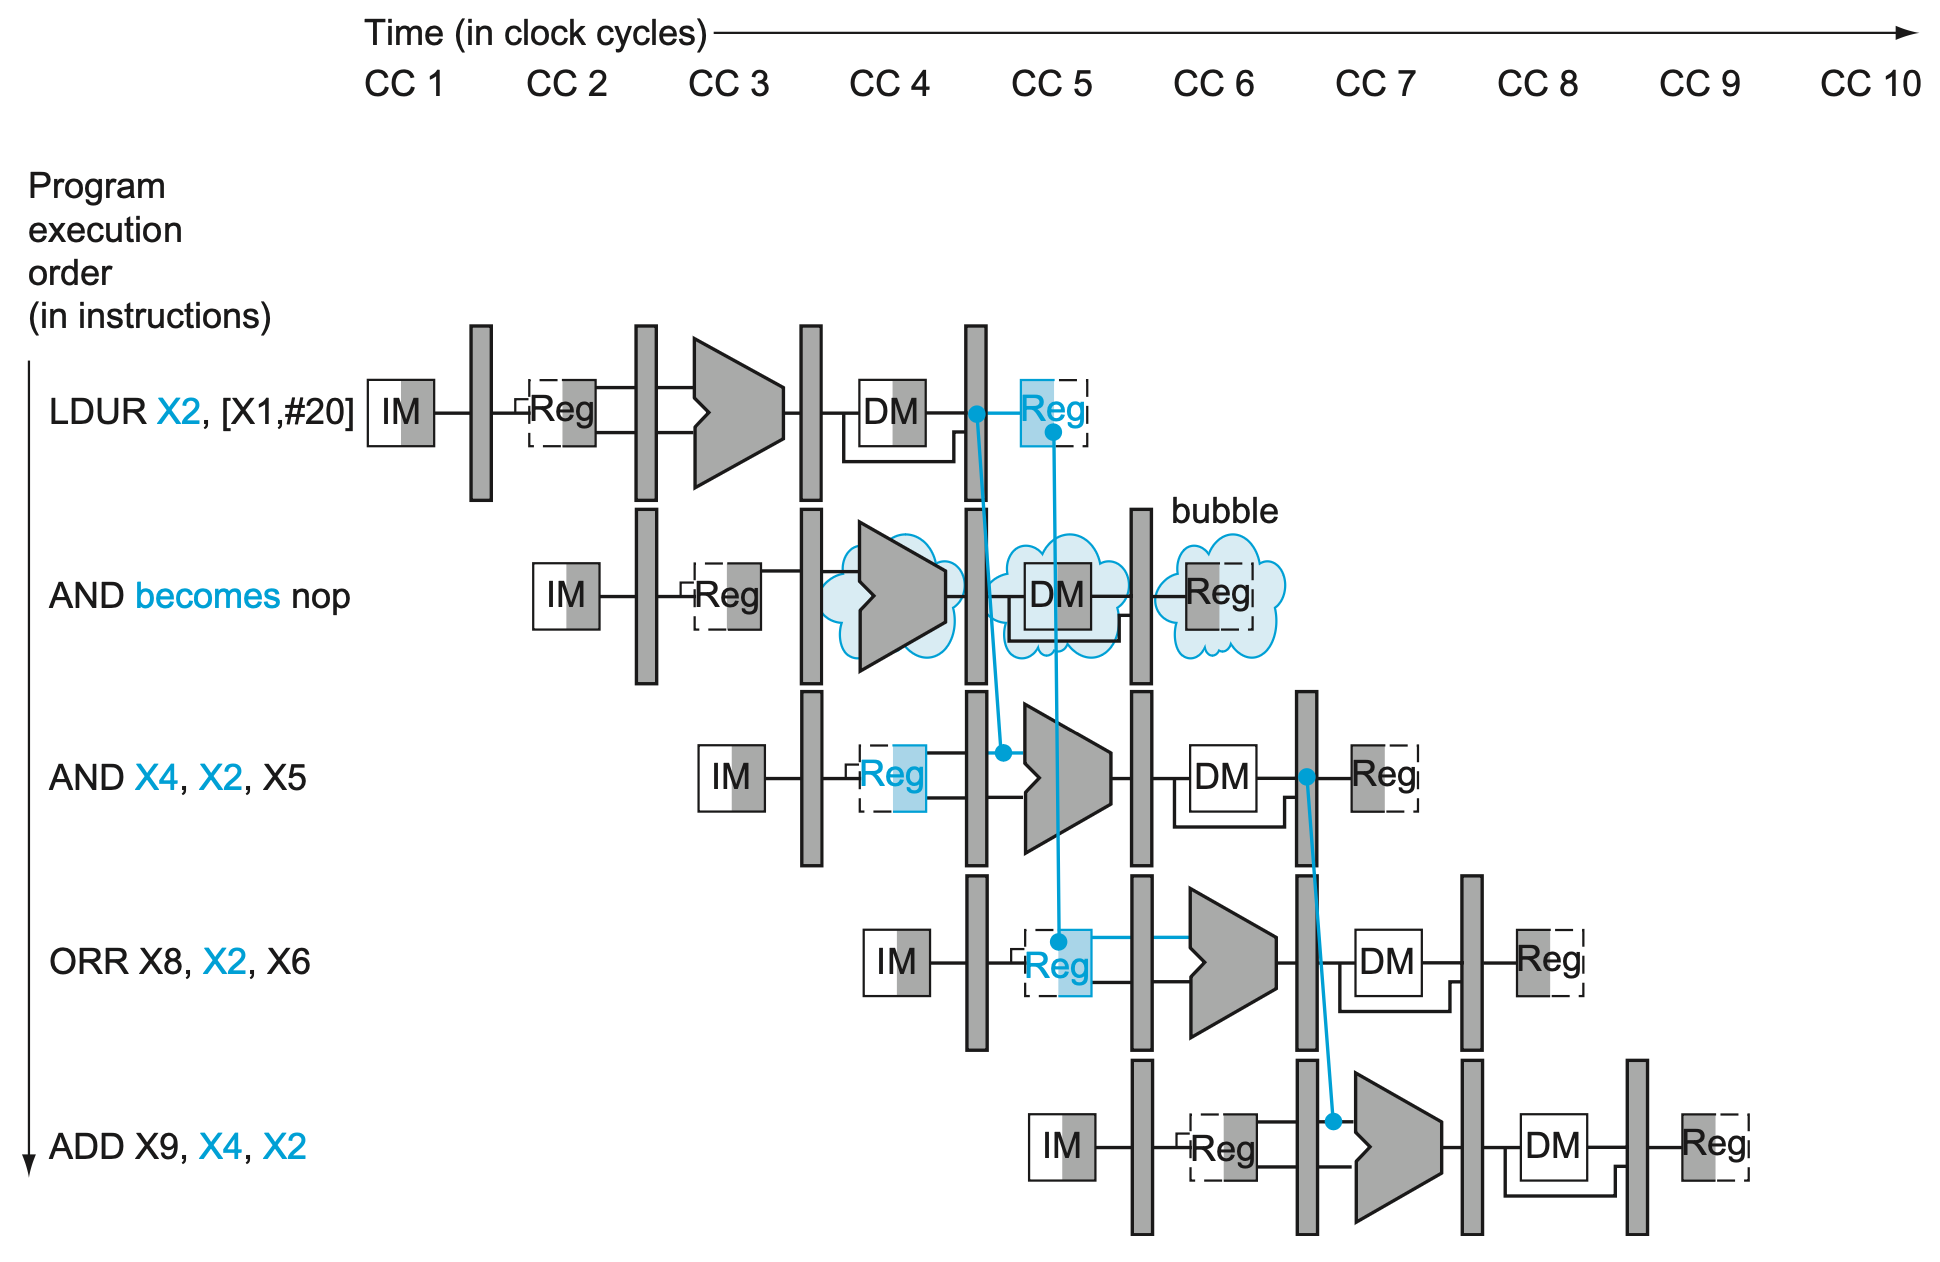
\includegraphics[width=0.5\linewidth]{img/stall-nop.png}
    }
    \caption{\textit{Example of \texttt{NOP} use for stalling and later forwarding}}
\end{figure}

\subsubsection*{\rightarrow \ \texttt{Control Hazards}}
\vspace{-0.5em}

When the fetched instruction is not the one needed (e.g. encountered branching).

Prediction is used to assume rather than wait for the branch to accertain the outcome, such as always not taking the branch.

Dynamic prediction differs in result depending of what happened before (keeping a history).

The penalty for an incorrect prediction is that the pipeline must restart from the proper branch address, stalling the process.

\begin{tcolorbox}[
    enhanced,
    attach boxed title to top left={xshift=6mm,yshift=-1.5mm},
    colback=moonstoneblue!20,
    colframe=moonstoneblue,
    colbacktitle=moonstoneblue,
    title=Simple Branch Prediction Methodologies,
    fonttitle=\bfseries\color{white},
    boxed title style={size=small,colframe=moonstoneblue,sharp corners},
    sharp corners,
    label=box:logic-types,
]
    {\color{moondark}\textbf{Branch not taken}}: Never takes a branch, and proceeds full speed when branch is not resolved (\textit{branch taken} is the opposite). \\
    {\color{moondark}\textbf{1-bit Dynamic branch}}: Keeps a 1-bit history of whether the branch was taken or not, and replicates latest behavior.
\end{tcolorbox}

Another two ways to predict are using 2-bit prediction, and tournament schemes (multiple predictions for a branch and they "compete").

With 2-bit predictions, there are 4 states of decisions: strongly taken, weakly taken, strongly not taken, weakly not taken. If "strongly", then if it is the opposite it will become "weakly", and if it is "weakly" then if it is the opposite it will become the other "weakly" (like two-step verification).

\begin{figure}[htbp]
    \centering
    \fcolorbox{codeframe}{white}{
       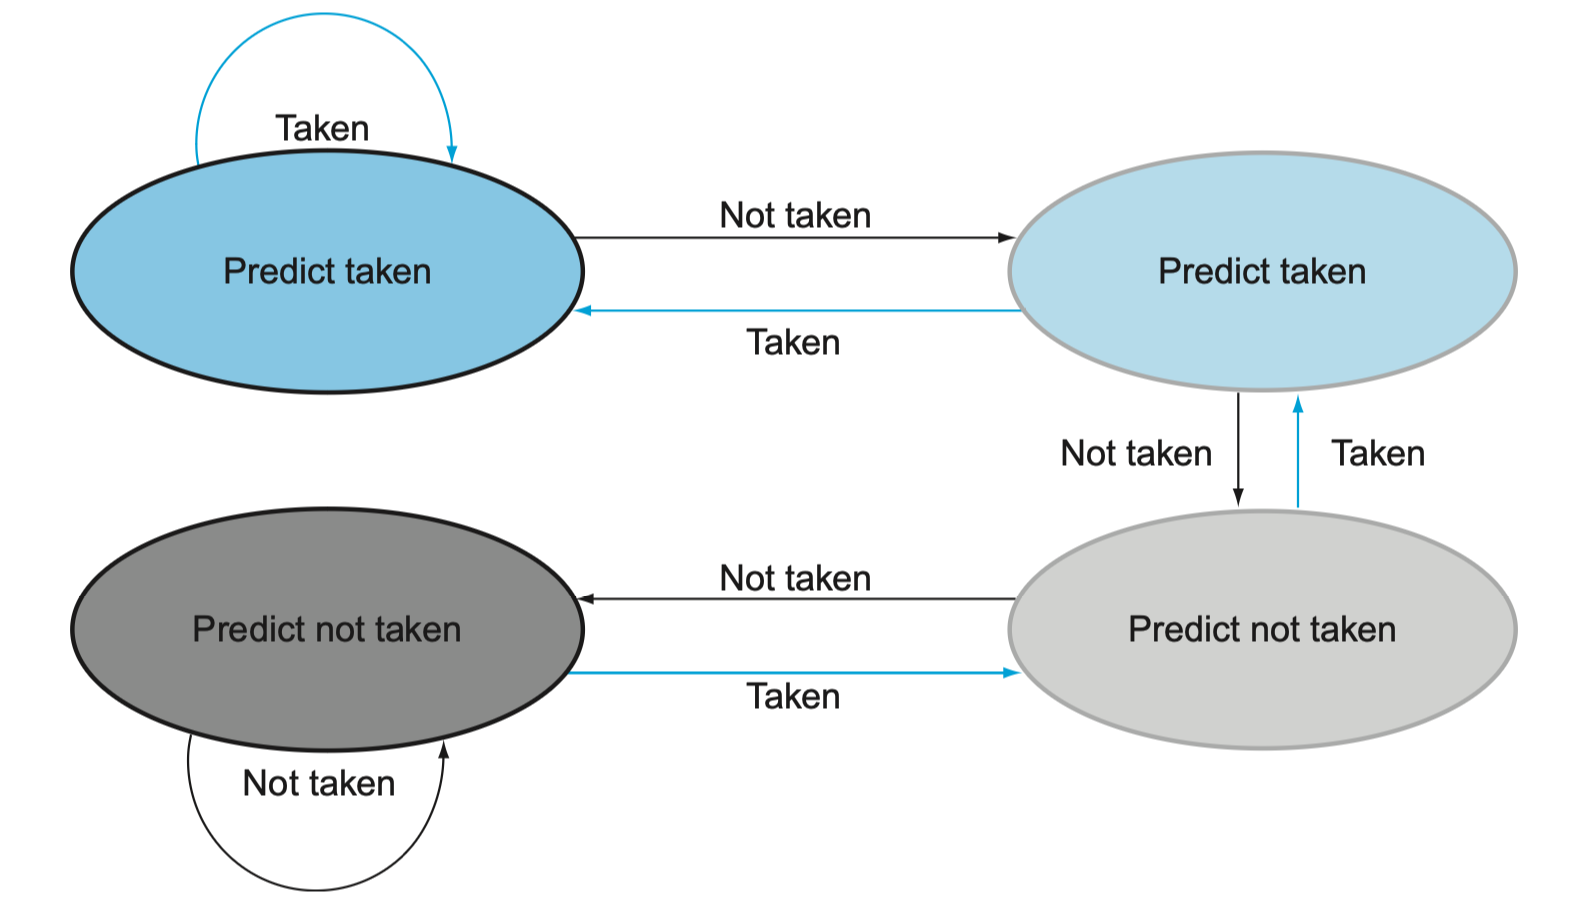
\includegraphics[width=0.5\linewidth]{img/two-bit-branch.png}
    }
    \caption{\textit{2-bit Branch Prediction Logic}}
\end{figure}

\section*{Chapter 5}
\addcontentsline{toc}{section}{Chapter 5}

The memory hierarchy has elements increasing in sizes and access times the further away from the processor they are. Derived from the locality principle.

\begin{figure}[htbp]
    \centering
    \fcolorbox{codeframe}{white}{
       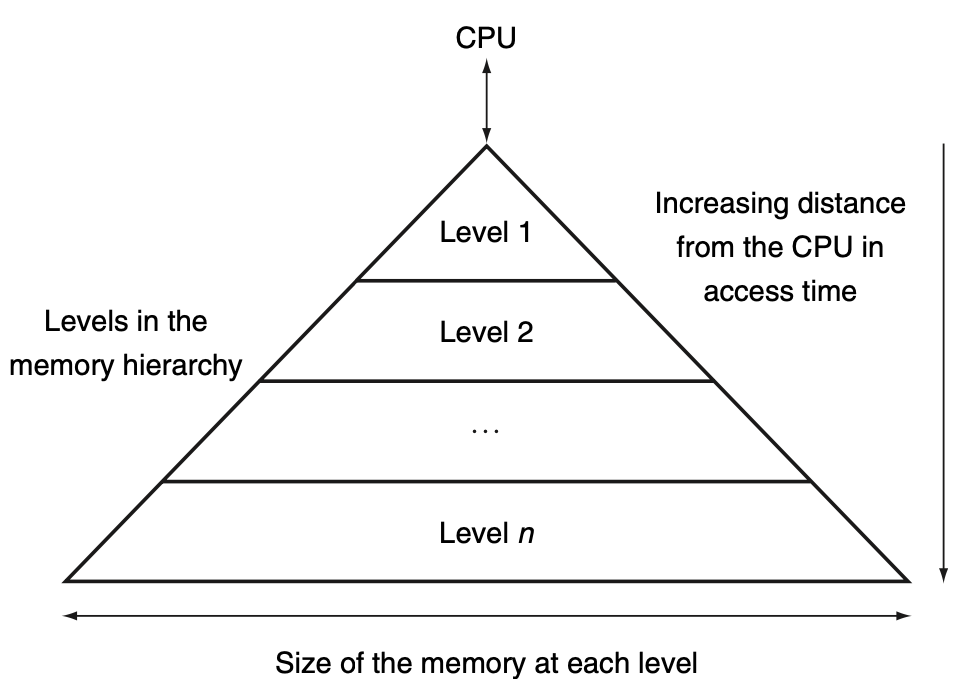
\includegraphics[width=0.5\linewidth]{img/mem-pyramid.png}
    }
    \caption{\textit{2-bit Branch Prediction Logic}}
\end{figure}

\begin{tcolorbox}[
    enhanced,
    attach boxed title to top left={xshift=6mm,yshift=-1.5mm},
    colback=moonstoneblue!20,
    colframe=moonstoneblue,
    colbacktitle=moonstoneblue,
    title=Principle of Locality,
    fonttitle=\bfseries\color{white},
    boxed title style={size=small,colframe=moonstoneblue,sharp corners},
    sharp corners,
    label=box:logic-types,
]
    {\color{moondark}\textbf{Temporal}}: If an element is referenced, then it will tend to be referenced again very soon. \\
    {\color{moondark}\textbf{Spacial}}: If an element is referenced, then elements around it will tend to be referenced again very soon. \\
    \textit{Elements in this case refers to data locations.}
\end{tcolorbox}

\subsection*{SRAM}

Volatile memory arrays with a read/write port that have a fixed access time to any data.

They don't need refreshing (access time is close to cycle time) and they require minimal power to retain charge in standby.

\textit{Used to be used as caches, but nowadays caches are integrated onto the processor chip.}

\begin{figure}[htbp]
    \centering
    \fcolorbox{codeframe}{white}{
       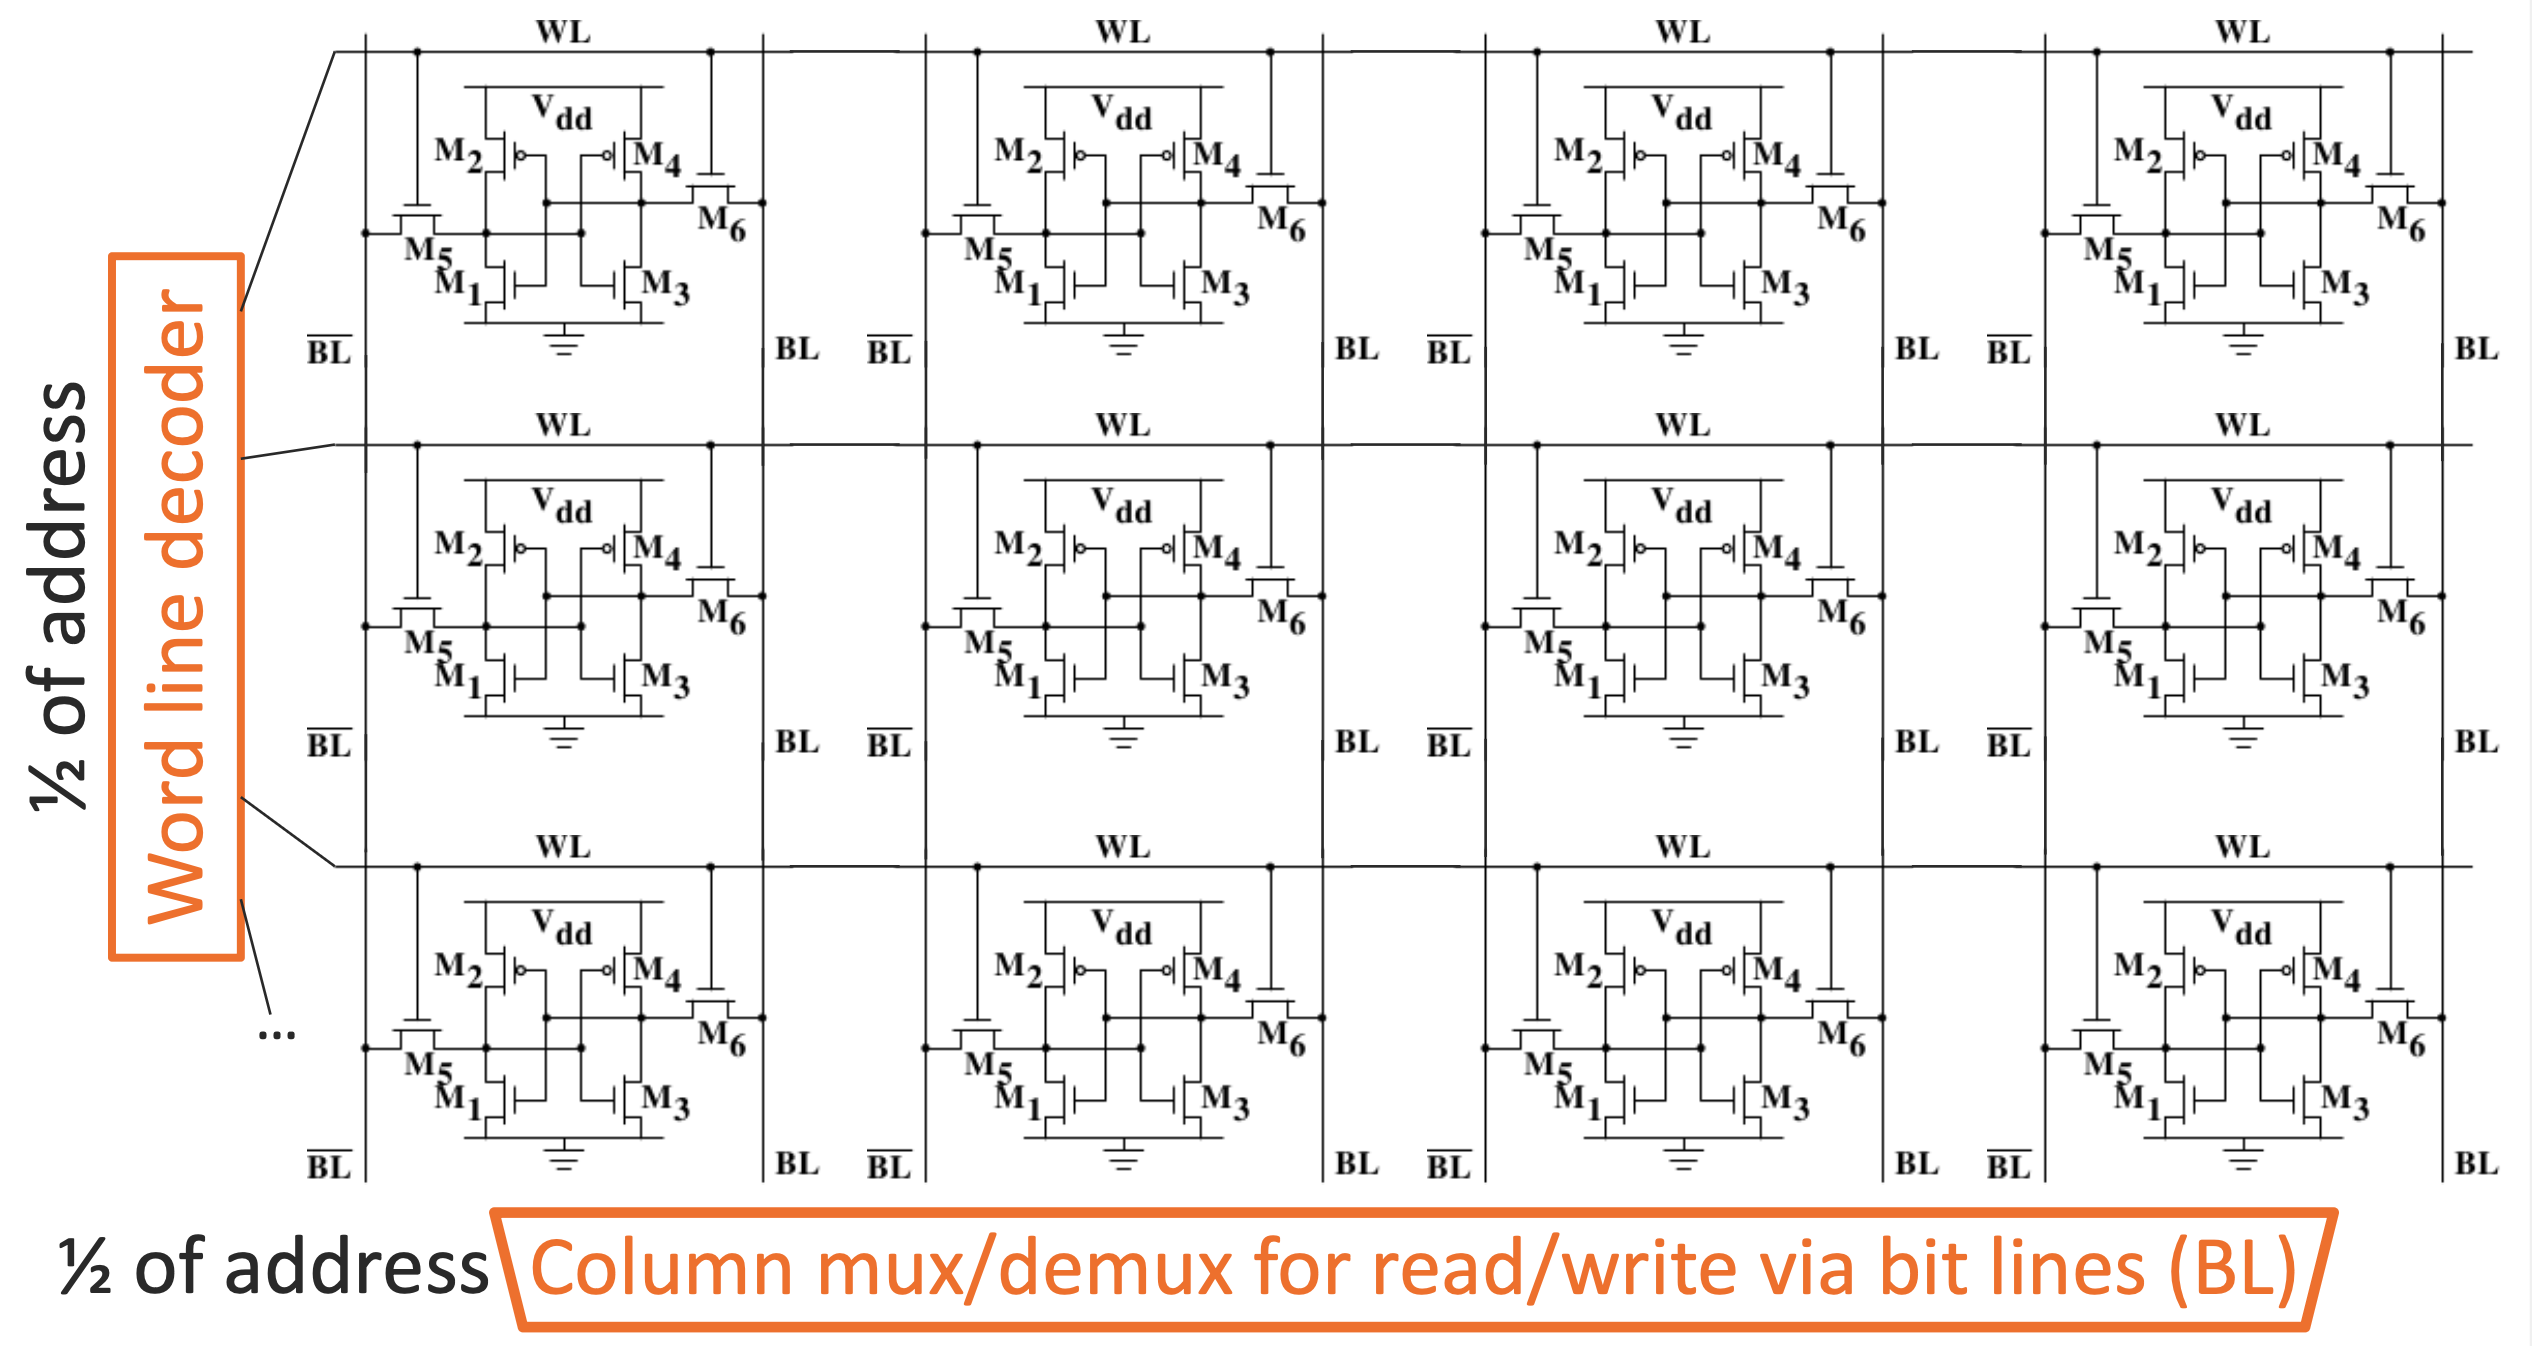
\includegraphics[width=0.5\linewidth]{img/sram-array.png}
    }
    \caption{\textit{SRAM array bit addressing}}
\end{figure}

For selection, there is a row (word-line MUX) and column decoder (column MUX/DEMUX).

$\rightarrow$ Row: Takes the higher order $k$ bits of the address and allows selection of $2^k$ rows.

$\rightarrow$ Column: Takes the remaining lower order $m$ bits and allows selection of $2^m$ columns.

\subsection*{DRAM}

Called \textit{dynamic} because it requires \underline{periodical refreshing} (read out and write in), in contrast to SRAM (static).

DRAM is volatile.

To save time, DRAM (made up of banks that can be accessed in parallel) refreshes entire rows at a time (two-level decoding) through fast buffers (SRAM-like).

\begin{figure}[htbp]
    \centering
    \fcolorbox{codeframe}{white}{
       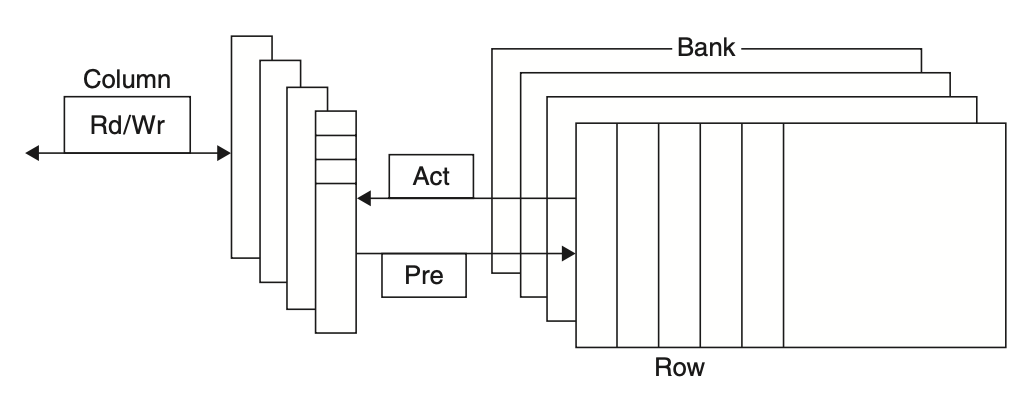
\includegraphics[width=0.5\linewidth]{img/internal-dram.png}
    }
    \caption{\textit{DRAM Banks and Row Buffering}}
\end{figure}

Once in a row buffer, you can access all data of the row by changing the column address at no major cost.

\textbf{SDRAM}s share clock signal (synchronous), which has faster and more predictable access times. \textit{No need for time negotiation overhead.}

\subsection*{Flash Memory}

Flash is non-volatile, RAM, and tough, particularly good for mobile devices.

Writes can wear out flash memory bits, thus it employs \underline{wear-leveling}: Remapping used blocks to less used blocks.

\subsection*{Disk Memory}

Non-volatile memory which surface is made of tracks (circles), read/written to through a small coil called a \textit{read-write head}.

The smallest unit of information read/written is a sector.

\textit{Principle of locality helps reduce avg. seek time (how much it takes in finding the correct track)}

\subsection*{Basics of Caches}

\textbf{Cache} refers to storage that takes advantage of locality of access. It can be understood as being guided by the following questions.

$\rightarrow$ Is the referenced block already in the cache?

$\rightarrow$ If so, where in the cache can I find it?

\subsection*{Direct Mapping Cache}

Each memory location is mapped to one location in the cache.
\vspace{-1em}
$$(\text{Block Address}) \mod (\text{Number of Blocks in the Cache})$$

Cache entries can be computed with the lower order k-bits, called the \textbf{index} (e.g. if number of blocks is 8, then you need $\log_{2}{8}=3$ bits).

\textbf{Tags} are additional identification to make sure that the word requested matches with the one stored in the cache. They are the upper bits remaining after indexing, stored in the cached entry, that gets compared with the request upon access (hit or miss).

\begin{figure}[htbp]
    \centering
    \fcolorbox{codeframe}{white}{
       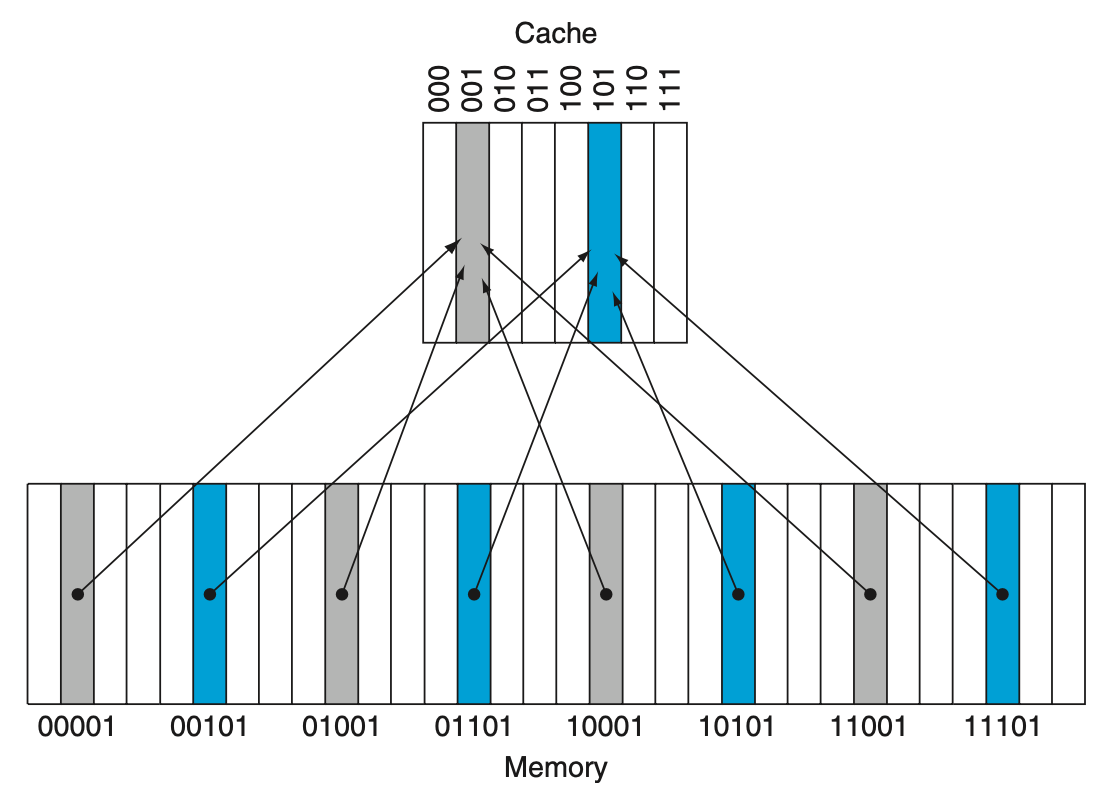
\includegraphics[width=0.5\linewidth]{img/direct-mapping-cache.png}
    }
    \caption{\textit{Direct Mapping Cache Block Addressing illustration}}
\end{figure}

There is also a \textbf{valid bit} to distinguish whether the cache entry has valid data (e.g. upon processor start up), and a \textbf{dirty bit} that indicates writes to a cache line after it was brought in (for things like updating the reference in main memory).

Caches benefit from \textit{temporal locality} as referenced words replace less than recently referenced ones.

Note that the cache address starts with a byte offset (needed later to index into sets and pick which block is needed).

\begin{figure}[htbp]
    \centering
    \fcolorbox{codeframe}{white}{
       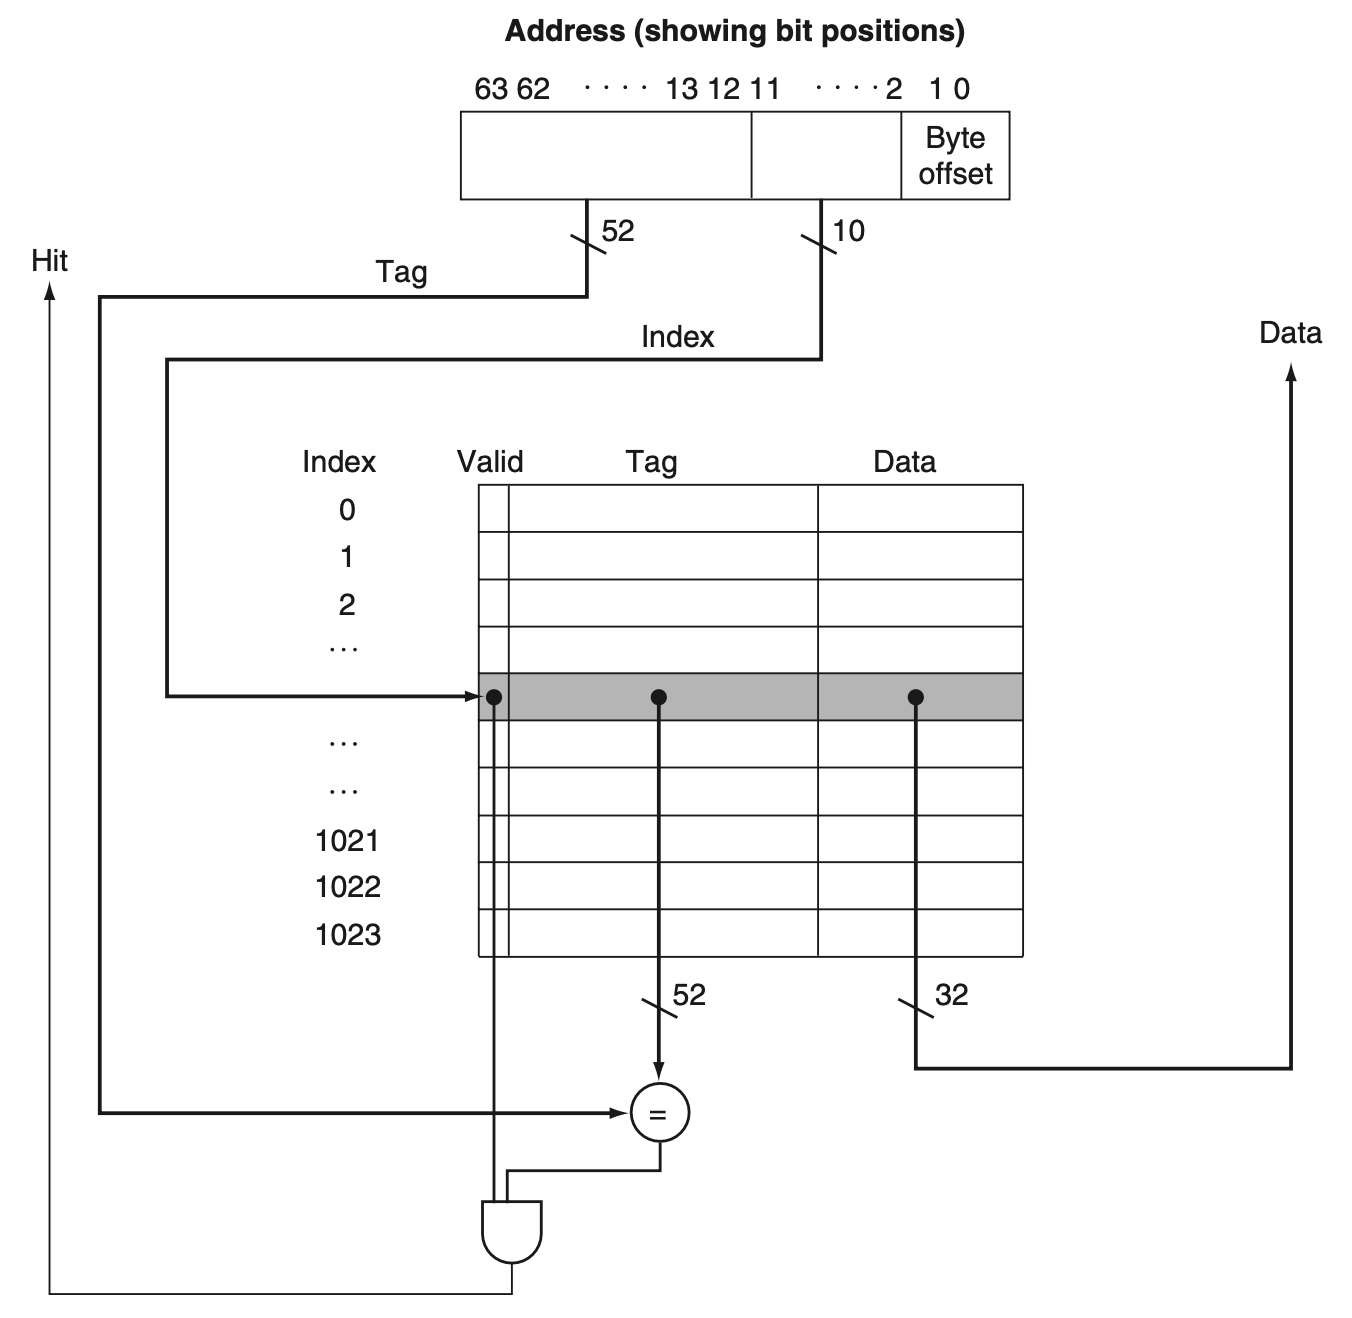
\includegraphics[width=0.5\linewidth]{img/cache-direct.png}
    }
    \caption{\textit{Diagram of Direct Mapping Cache and the relationship with the Address}}
\end{figure}

\pagebreak
The tag field will have the following size for 64-bit addresses, where there are $n$ index bits ($2^n$ blocks), $m$ bits to address the $2^{m}$ words,and $m+2$ for addressing one of the 4 bytes per word.
\vspace{-1em}
$$64-(n+m+2)$$

Thus the total number of \underline{bits} in a directly-mapped cache is \\
\begin{*align}
  2^n \times (BlockSize + TagSize + ValidFieldSize)\\
  2^n \times \bigl((2^m \times 2^2\,\text{bytes}\times 2^3\,\text{bits}) + (64-n-m-2) + 1\bigr)\\
  2^n \times \bigl((2^m \times 32) + (64-n-m-2) + 1\bigr)
\end{*align}

Larger blocks can exploit spacial locality to lower miss rates. When the improvement slows down, the miss penalty overwhelms the lower rates.

\begin{tcolorbox}[
    enhanced,
    attach boxed title to top left={xshift=6mm,yshift=-1.5mm},
    colback=moonstoneblue!20,
    colframe=moonstoneblue,
    colbacktitle=moonstoneblue,
    title=Cache Write Handling,
    fonttitle=\bfseries\color{white},
    boxed title style={size=small,colframe=moonstoneblue,sharp corners},
    sharp corners,
    label=box:logic-types,
]
    {\color{moondark}\textbf{Write-through}}: Writes update both the cache and the next lower level in the memory hierarchy using a \textbf{write buffer} to avoid stalls due to overhead in writing to lower memory. \\
    {\color{moondark}\textbf{Write-back}}: Replaces the written value in the cache to lower memories when the block is replaced.
\end{tcolorbox}

\pagebreak
\subsection*{Cache Misses}

\begin{tcolorbox}[
    enhanced,
    attach boxed title to top left={xshift=6mm,yshift=-1.5mm},
    colback=moonstoneblue!20,
    colframe=moonstoneblue,
    colbacktitle=moonstoneblue,
    title=The 3 C's,
    fonttitle=\bfseries\color{white},
    boxed title style={size=small,colframe=moonstoneblue,sharp corners},
    sharp corners,
    label=box:logic-types,
]
    {\color{moondark}\textbf{Compulsory miss}}: Unavoidable miss that occurs when first loading a block into the cache (e.g. on processor startup). \\
    {\color{moondark}\textbf{Capacity miss}}: Cache is too small to hold the required block. \\
    {\color{moondark}\textbf{Conflict miss}}: Competing for the same memory address due to cache design (even if the cache is large enough).
\end{tcolorbox}

Compulsory misses can be improved by increasing the size per block in the cache (less blocks used by the program) or load through prediction.

Solutions to conflict misses is to add more slots/sets to a particular index (k-associative design).

To illustrate how performance is affected through hits and misses, AMAT is used.
\vspace{-1em}
$$AMAT = TimeForHit + MissRate \times MissPenalty$$

\subsection*{Set \& Full Associative Cache}

For \textbf{set-associative}, there are n-sets (where $n\ge 1$) that are mapped by the index, that contain k number of blocks that will perform tag comparisons against the requested block's tag.

\textbf{Full associative} does not perform a direct mapping by the index, but rather requires a search, as a block can be placed in any location of the cache (equivalent of using 1 set that holds all block locations).

\begin{figure}[htbp]
    \centering
    \fcolorbox{codeframe}{white}{
       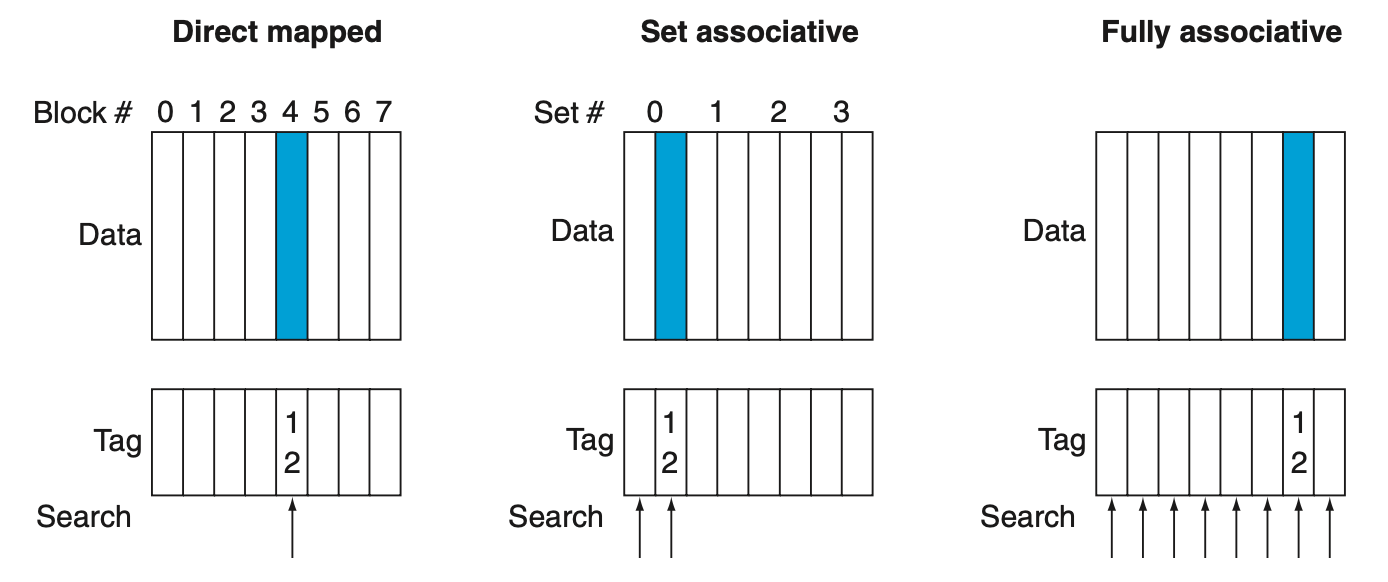
\includegraphics[width=0.5\linewidth]{img/cache-access.png}
    }
    \caption{\textit{Example of Memory access with the three different Cache designs}}
\end{figure}

A more detailed look into the memory hierarchy.

\pagebreak
\begin{figure}[htbp]
    \centering
    \fcolorbox{codeframe}{white}{
       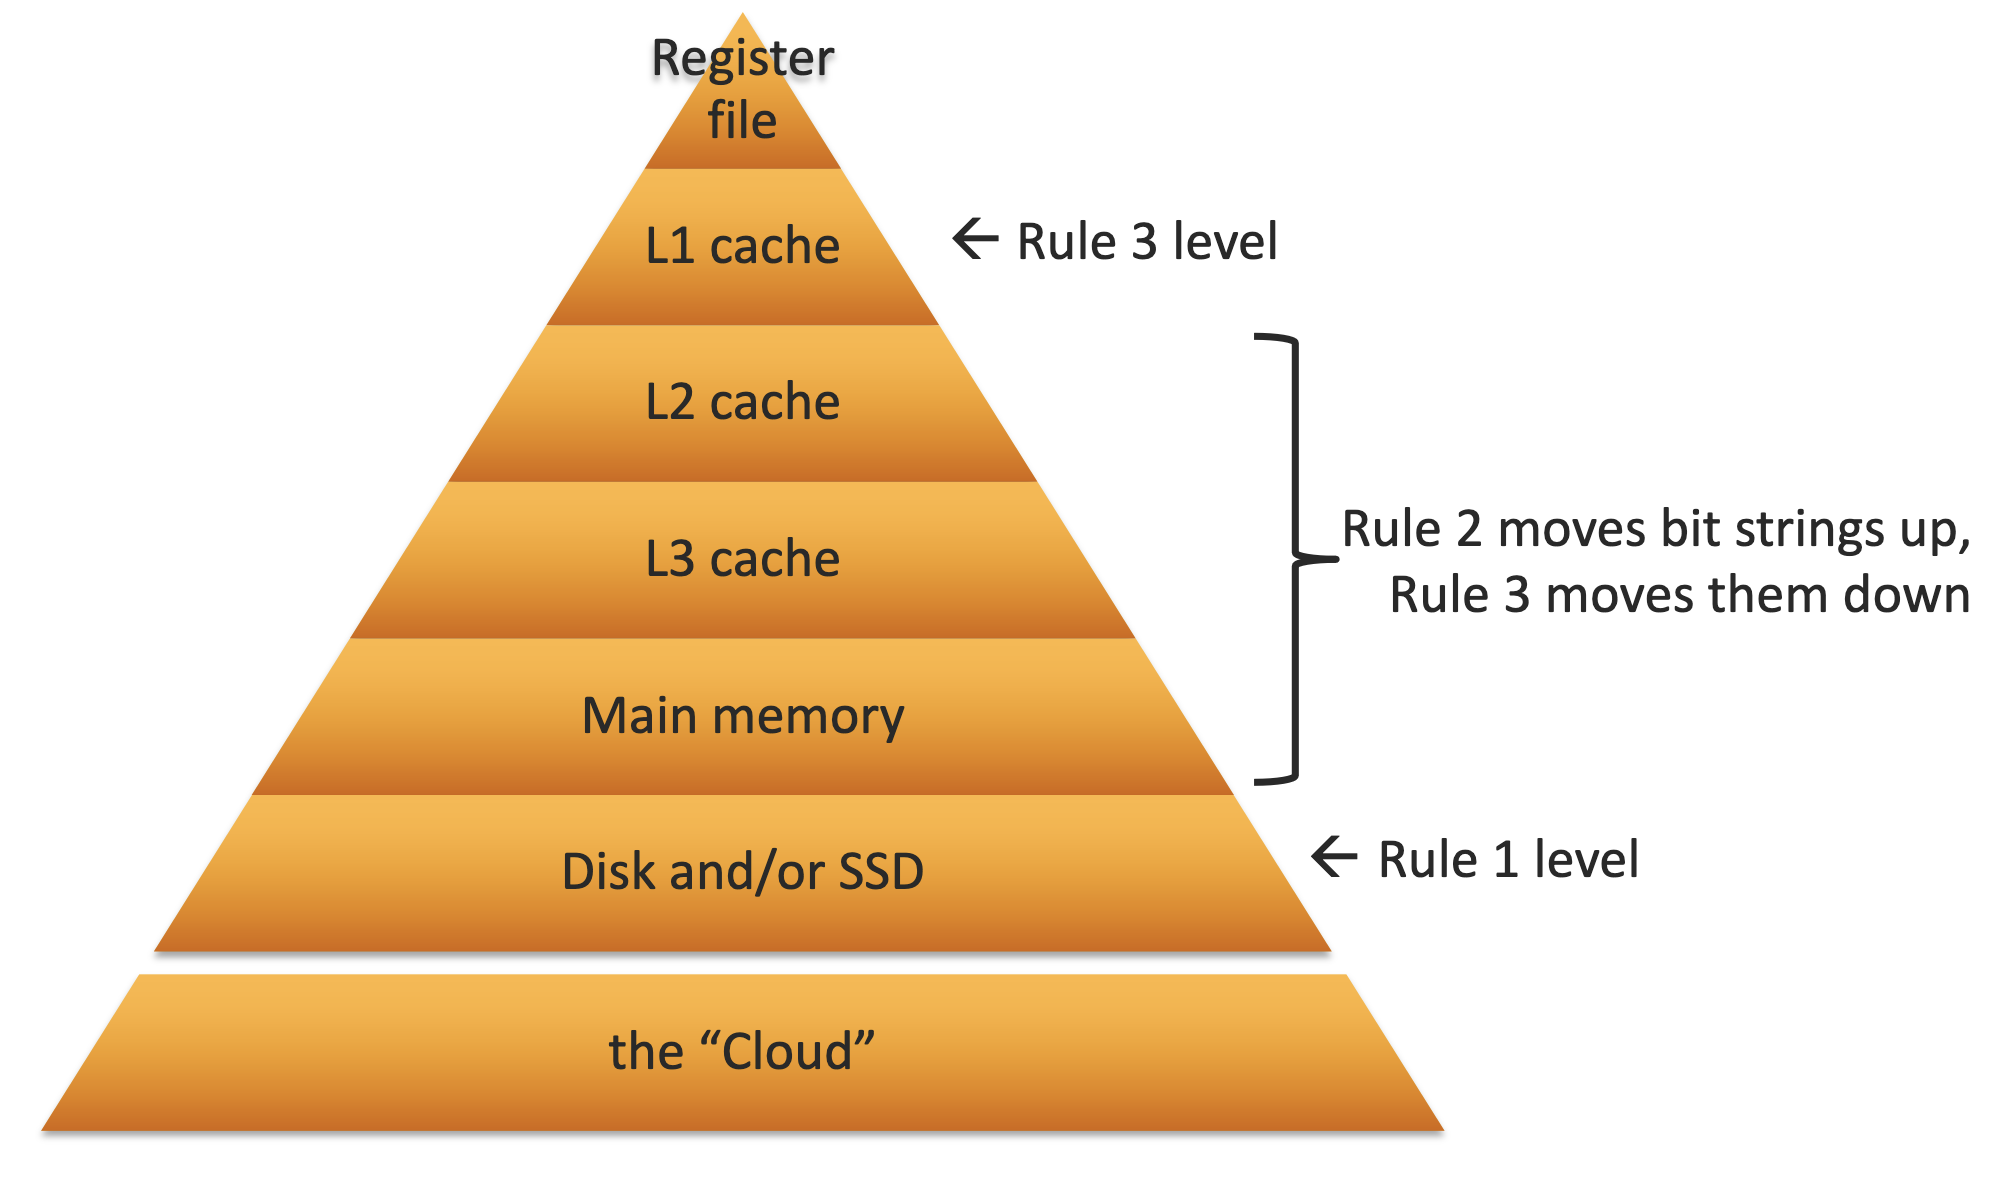
\includegraphics[width=0.7\linewidth]{img/memh-detailed.png}
    }
    \caption{\textit{Example of Memory access with the three different Cache designs}}
\end{figure}

\subsection*{Virtual Memory}

Main memory has limited space, so \textbf{virtual memory} treats it like a "cache relative to secondary storage" (handles managing the two memories).

To enforce protection between different programs, virtual memory allows all programs to have their own \textbf{address space}, which addresses will get translated into \textit{physical addresses} (relocation).

If it is not mapped to main memory, then it gets mapped to secondary regions (e.g. disk).

\begin{figure}[htbp]
    \centering
    \fcolorbox{codeframe}{white}{
       \includegraphics[width=0.5\linewidth]{img/vm-translation.png}
    }
    \caption{\textit{Pages mapped from Virtual addresses to Physical addresses}}
\end{figure}

When a virtual memory block requested is not in main memory there is a \textbf{page fault}.

Virtual memory addresses are made of the \textit{virtual page number} (high-order bits) and a \textit{page offset} (low-order bits).

$\rightarrow$ The page offset remains unchanged when translating from virtual to physical addresses and is used to obtain information directly from page.

$\rightarrow$ The virtual page number (VPN) has more bits, and thus maps to more locations than the physical page number (main memory vs secondary memory). Illusion of unbounded memory.

\begin{figure}[htbp]
    \centering
    \fcolorbox{codeframe}{white}{
       \includegraphics[width=0.5\linewidth]{img/vm-addressing.png}
    }
    \caption{\textit{Virtual address translation to Physical addresses}}
\end{figure}

Physical memory is stored in three parts: OS, page table, page frames (largest).

\begin{figure}[htbp]
    \centering
    \fcolorbox{codeframe}{white}{
       \includegraphics[width=0.4\linewidth]{img/physical-mem.png}
    }
    \caption{\textit{Virtual address translation to Physical addresses}}
\end{figure}

\subsection*{Page Tables}

To find the corresponding physical page number (PPN) from a VPN, we use \textbf{page tables}, seen in the \autoref{fig:page-table}.

\begin{tcolorbox}[
    enhanced,
    attach boxed title to top left={xshift=6mm,yshift=-1.5mm},
    colback=moonstoneblue!20,
    colframe=moonstoneblue,
    colbacktitle=moonstoneblue,
    title=Step by Step on Page Table Indexing,
    fonttitle=\bfseries\color{white},
    boxed title style={size=small,colframe=moonstoneblue,sharp corners},
    sharp corners,
    label=box:logic-types,
]
    {\color{moondark}\textbf{1. VPN gets aligned with Page Table}}: VPN gets multiplied by the size of a PTE (page table entry), and then gets added to the base of the page table stored in the Page Table register (like an array entry). \\
    {\color{moondark}\textbf{2. Mapping and access of PPN}}: There can be either a \texttt{NOT PRESENT} (causing a page fault) or a PPN (valid bit) indexed at the VPN offset calculated.
\end{tcolorbox}

\pagebreak

\begin{figure}[htbp]
    \centering
    \fcolorbox{codeframe}{white}{
       \includegraphics[width=0.5\linewidth]{img/vm-page-table.png}
    }
    \caption{\textit{Page Table illustration with a valid bit to determine entry}}
    \label{fig:page-table}
\end{figure}

The problem with design is that it will generate a massive page table (too big to fit in RAM), so the solution is to add multi-level page tables.

$\rightarrow$ \underline{First level page table} (page-directory) is allocated always, and will point to second level page tables.

$\rightarrow$ \underline{Second level page tables} are allocated as they are used, and point to another level or the physical memory address needed.

\begin{figure}[htbp]
    \centering
    \fcolorbox{codeframe}{white}{
       \includegraphics[width=0.5\linewidth]{img/multi-level-paging.png}
    }
    \caption{\textit{Multi-level Page Table illustration}}
\end{figure}

\begin{figure}[htbp]
    \centering
    \fcolorbox{codeframe}{white}{
       \includegraphics[width=0.5\linewidth]{img/multi-level-table-split.png}
    }
    \caption{\textit{Multi-level Page Table address field}}
\end{figure}

A way to speed up this process is using the TLB (translation lookaside buffer) that acts like a full-associative cache into the page-directory.

Fully-associative as conflict misses will turn into capacity misses (capacity required is low).

For improving TLB lookups we can use the CAM (content addressable memory) that, in constant time, gets a key and does parallel comparisons will all CAM entries.

$\rightarrow$ Upon hit it gives the PPN and metadata (e.g. SIGSEGV detection), and upon miss it uses the page-directory.

CAM is expensive and is organized as N m-bit slots, where N and m are chosen by need.

\begin{figure}[htbp]
    \centering
    \fcolorbox{codeframe}{white}{
       \includegraphics[width=0.5\linewidth]{img/vm-cam.png}
    }
    \caption{\textit{CAM structure for constant time parallel access}}
\end{figure}

\subsection*{Page Faults}

The additional mappings by the VPN, that are not to main memory, map to the \textbf{swap space} (on disk or flash).

When a page fault occurs the OS will add the \textit{least recently used} page (prediction).

\pagebreak
\begin{figure}[htbp]
    \centering
    \fcolorbox{codeframe}{white}{
       \includegraphics[width=0.5\linewidth]{img/full-page-table.png}
    }
    \caption{\textit{Page Table that maps to main memory and swap space}}
\end{figure}

The MMU (memory management unit) makes up the page table register and the TLB, and will send the page fault signal (upon miss) to the OS, who then calls the page fault handler.

Handling page faults takes a lot of time.

\subsection*{Bus Errors}

Following of what was said about buses \hyperref[jmp:buses-general]{before}, there are potential errors that can arise.

\begin{tcolorbox}[
    enhanced,
    attach boxed title to top left={xshift=6mm,yshift=-1.5mm},
    colback=moonstoneblue!20,
    colframe=moonstoneblue,
    colbacktitle=moonstoneblue,
    title=Bus errors,
    fonttitle=\bfseries\color{white},
    boxed title style={size=small,colframe=moonstoneblue,sharp corners},
    sharp corners,
    label=box:logic-types,
]
    {\color{moondark}\textbf{Address conflicts}}: Two different elements/devices respond to the same address bus. \\
    {\color{moondark}\textbf{Unassigned address}}: No devices respond to a given address.
\end{tcolorbox}

\pagebreak
\section*{Week 12 Slides}
\addcontentsline{toc}{section}{Week 12}

Interrupts are built in hardware, that saves the current pointer, jumps to code for the interrupt, and resumes execution from when \textit{return from interrupt} is reached.

\subsection*{Device Drivers}

The \textbf{device driver} is software that communicates with a device: initializes the device, CSRs (control \& status registers) are set to start I/O ops, and handles device interrupts.

\begin{tcolorbox}[
    enhanced,
    attach boxed title to top left={xshift=6mm,yshift=-1.5mm},
    colback=moonstoneblue!20,
    colframe=moonstoneblue,
    colbacktitle=moonstoneblue,
    title=Purpose of Device Drivers,
    fonttitle=\bfseries\color{white},
    boxed title style={size=small,colframe=moonstoneblue,sharp corners},
    sharp corners,
    label=box:logic-types,
]
    {\color{moondark}\textbf{Encapsulation}}: Creates an interface for wrapping up the details of how to talk to a device. \\
    {\color{moondark}\textbf{Hiding}}: Hides what happens under the hood. \\
    {\color{moondark}\textbf{Independence}}: No dependence on the design of any device (generic).
\end{tcolorbox}

The structure of a device driver: lower half, upper half, and shared variables.

$\rightarrow$ \underline{Lower half}: Handler code invoked during interrupt (direct communication to device).

$\rightarrow$ \underline{Upper half}: Functions invoked by applications (I/O requests).

$\rightarrow$ \underline{Shared variables}: Used by both halves with input and output buffers.

\begin{figure}[htbp]
    \centering
    \fcolorbox{codeframe}{white}{
       \includegraphics[width=0.6\linewidth]{img/device-driver.png}
    }
    \caption{\textit{Device driver structure}}
\end{figure}

\begin{tcolorbox}[
    enhanced,
    attach boxed title to top left={xshift=6mm,yshift=-1.5mm},
    colback=moonstoneblue!20,
    colframe=moonstoneblue,
    colbacktitle=moonstoneblue,
    title=Types of Devices,
    fonttitle=\bfseries\color{white},
    boxed title style={size=small,colframe=moonstoneblue,sharp corners},
    sharp corners,
    label=box:logic-types,
]
    {\color{moondark}\textbf{Character oriented}}: Transfer one byte at a time (e.g. keyboards). \\
    {\color{moondark}\textbf{Block oriented}}: Transfer blocks of data at a time (e.g. disks, network interfaces).
\end{tcolorbox}

\subsection*{Output Request Queue}

There is a queue shared by both halves (shared variables), where the top enqueues (when the application issues I/O) and the bottom dequeues the next request (starting it).






























































% \begin{lstlisting}[caption={Simple SIGINT handler}]
% unsigned char stop = 0;
%
% void signal_handler(int x) {
%     stop = 1;
% }
%
% int main(void) {
%     signal(SIGINT, signal_handler);
%
%     /* Pressing Ctrl-C invokes signal_handler() */
%
%     while (!stop);
%     return 0;
% }
% \end{lstlisting}
%
% This is an example of an image.
%
% \begin{figure}[htbp]
%   \centering
%
%   \fcolorbox{codeFrame}{white}{%
%     \includegraphics[width=0.5\linewidth]{img/graph.png}%
%   }
%
%   \caption{My example image}
%   \label{fig:example}
% \end{figure}



\end{document}
